\chapter{Desarrollo}

\section{Modelo matemático del PMSM}

En esta sección, se abordará de manera gradual la introducción al control vectorial de máquinas eléctricas. Esta sección se asemeja más a un conjunto de pasos para comprender completamente el control utilizado en los inversores. Es importante tener en cuenta que existen muchas simplificaciones matemáticas, suposiciones no justificadas y pasos omitidos ya que la extensión de la sección sería extremadamente larga en caso de razonar desde cero todos los resultados.

\subsection{Marco de referencia estático}

Los motores síncronos de imanes permanentes (PMSM) están hechos de hierro, cobre y imanes. Se limita el análisis a máquinas de tres fases, aunque el análisis para sistemas con más de tres fases es similar. El cobre se distribuye en devanados, que tienen una resistencia y una inductancia iguales entre ellas si la máquina está equilibrada. Además, cuando el rotor gira, los imanes permanentes inducen una tensión en los devanados, lo que se conoce como fuerza contraelectromotriz (FCEM).

Se trabajará con motores cuyos devanados estén conectados en configuración estrella, ya que se utiliza con mucha más frecuencia que la configuración delta. De todas maneras, es sencillo extender el modelo y el control a motores con conexión delta.


\begin{figure}[H]
	\centering
	\begin{circuitikz}
		% Draw three phases
		\draw (0,0) to [L, l=$L_s$, o-] ++(2,0) to [R, l=$R_s$] ++(2,0) to [sV, v=$e_a$, invert] ++(2,0) -- ++(0,-2){};
		
		\draw (0,-2) to [L, l=$L_s$, o-] ++(2,0) to [R, l=$R_s$] ++(2,0) to [sV, v=$e_b$, invert] ++(2,0) -- ++(0,2);
		
		\draw (0,-4) to [L, l=$L_s$, o-] ++(2,0) to [R, l=$R_s$] ++(2,0) to [sV, v=$e_c$, invert] ++(2,0) -- ++(0,2);
		
		% Draw neutral point
		\draw (6,-2) node[circ]{} -- ++(0.5,0) node[circ]{} node[right]{$N$};
	\end{circuitikz}
	\caption{Circuito eléctrico equivalente de un PMSM trifásico en configuración estrella.}
\end{figure}

\subsection{Representación en el espacio vectorial}

Cuando el PMSM gira, las formas de onda de corriente y voltaje son aproximadamente sinusoidales. Siendo un sistema trifásico y equilibrado, se vería algo como en la siguiente figura.

\begin{figure}[H]
    \centering
    \hspace*{-1.5cm}
    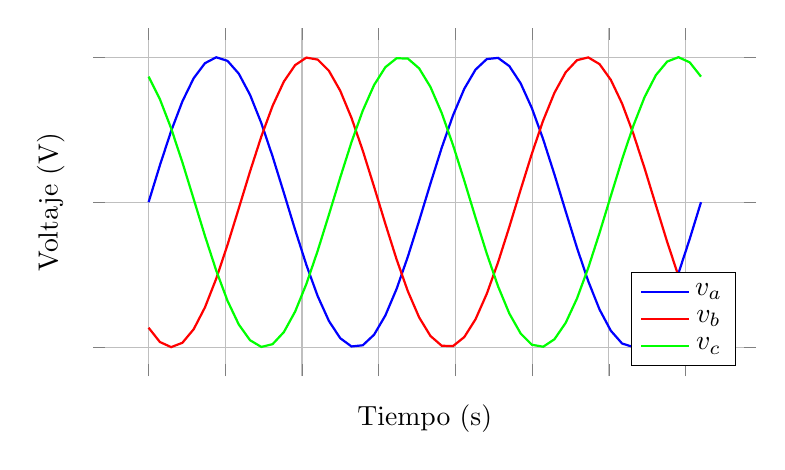
\begin{tikzpicture}
    \begin{axis}[
        width=10cm,
        height=6cm,
        xlabel={Tiempo (s)},
        ylabel={Voltaje (V)},
        legend entries={$v_a$, $v_b$, $v_c$},
        grid=major,  
        legend pos=south east,
        samples=50,
        domain=0:2*360,
        axis line style={draw=none},  % Elimina el recuadro exterior
        xticklabels=\empty,  % Elimina las marcas en el eje x
        yticklabels=\empty,  % Elimina las marcas en el eje y
    ]
    \addplot[blue, thick, domain=0:2*360] {sin(x)};
    \addplot[red, thick, domain=0:2*360] {sin(x - 120)};
    \addplot[green, thick, domain=0:2*360] {sin(x - 240)};
    \end{axis}
    \end{tikzpicture}
    \caption{Sistema trifásico representado en el tiempo.}
\end{figure}

Todas las ecuaciones se pueden definir a partir de este modelo, pero se vuelve muy poco práctico para análisis más complejos. Se introduce una forma de representar estas formas de onda en el espacio tridimensional $\mathbb{R}^3$, en el que se escogen los ejes \((a, b, c)\). Lo que debería esperarse ver es una forma tridimensional en el espacio $\mathbb{R}^3$. Se comienza en \(t = 0\) y se dibuja un punto en las coordenadas \([v_a(0), v_b(0), v_c(0)]\). Luego, se continúa trazando puntos mientras se avanza a lo largo del eje del tiempo. La forma se puede expresar como curva paramétrica como \([v_a(t), v_b(t), v_c(t)]\). Cuando se representa la forma resultante, puede sorprender, ya que es un círculo perfectamente plano. Cabe destacar que el orden de los ejes depende del contexto, y en este trabajo se toma el sistema de referencia mostrado en las siguientes figuras.


\begin{figure}[H]
    \centering
    \begin{subfigure}[b]{3cm}
        \centering
        \hspace*{-1.5cm}
        \begin{tikzpicture}
        \begin{axis}[
            %view={-45}{-35},
            view={-20}{-15},
            %view={54.74}{-15},
            axis lines=none,
            xmin=-1.5,
            xmax=1.5,
            ymin=-1.5,
            ymax=1.5,
            zmin=-1.5,
            zmax=1.5,
            no markers,
            axis equal,
            enlargelimits={upper=0.2},
            scale=1,
        ]
        \addplot3+[red, thick, no markers, samples=30, domain=-pi:pi, variable=\t]
            ({sin(deg(\t))}, {sin(deg(\t + 2*pi/3))}, {sin(deg(\t - 2*pi/3))});
       	
       % Ejes abc
       \draw[red, line width=1.5pt, -{Latex[length=1.5mm,width=1mm]}] (axis cs:0, 0, 0) -- (axis cs:0.5, 0, 0) node[pos=1.5]{$b$};
       \draw[red, line width=1.5pt, -{Latex[length=1.5mm,width=1mm]}] (axis cs:0, 0, 0) -- (axis cs:0, 0.5, 0) node[pos=1.5]{$a$};
       \draw[red, line width=1.5pt, -{Latex[length=1.5mm,width=1mm]}] (axis cs:0, 0, 0) -- (axis cs:0, 0, 0.5) node[pos=1.5]{$c$};
       
       \addplot3[draw=gray, no markers] coordinates {(-1.1, -1.1, -1.1) (-1.1, 1.1, -1.1)};
        \addplot3[draw=gray, no markers] coordinates {(-1.1, 1.1, -1.1) (1.1, 1.1, -1.1)};
        \addplot3[draw=gray, no markers] coordinates {(1.1, 1.1, -1.1) (1.1, -1.1, -1.1)};
        \addplot3[draw=gray, no markers] coordinates {(1.1, -1.1, -1.1) (-1.1, -1.1, -1.1)};
        \addplot3[draw=gray, no markers] coordinates {(-1.1, -1.1, 1.1) (-1.1, 1.1, 1.1)};
        \addplot3[draw=gray, no markers] coordinates {(-1.1, 1.1, 1.1) (1.1, 1.1, 1.1)};
        \addplot3[draw=gray, no markers] coordinates {(1.1, 1.1, 1.1) (1.1, -1.1, 1.1)};
        \addplot3[draw=gray, no markers] coordinates {(1.1, -1.1, 1.1) (-1.1, -1.1, 1.1)};
        \addplot3[draw=gray, no markers] coordinates {(-1.1, -1.1, -1.1) (-1.1, -1.1, 1.1)};
        \addplot3[draw=gray, no markers] coordinates {(-1.1, 1.1, -1.1) (-1.1, 1.1, 1.1)};
        \addplot3[draw=gray, no markers] coordinates {(1.1, 1.1, -1.1) (1.1, 1.1, 1.1)};
        \addplot3[draw=gray, no markers] coordinates {(1.1, -1.1, -1.1) (1.1, -1.1, 1.1)};
        \end{axis}
        \end{tikzpicture}
    \end{subfigure}
    \hfill
    \begin{subfigure}[b]{3cm}
        \centering
            \hspace*{-1.5cm}
            \begin{tikzpicture}
            \begin{axis}[
                view={-45}{-35},
                %view={-20}{-15},
                %view={54.74}{-15},
                axis lines=none,  % Elimina los ejes
                xmin=-.9,
                xmax=.9,
                ymin=-.9,
                ymax=.9,
                zmin=-.9,
                zmax=.9,
                no markers,
                axis equal,
                enlargelimits={upper=0.2},
                scale=1,
            ]
            \addplot3+[red, thick, no markers, samples=30, domain=-pi:pi, variable=\t]
                ({sin(deg(\t))}, {sin(deg(\t + 2*pi/3))}, {sin(deg(\t - 2*pi/3))});
           
           	% Ejes abc
           	\draw[red, line width=1.5pt, -{Latex[length=1.5mm,width=1mm]}] (axis cs:0, 0, 0) -- (axis cs:0.5, 0, 0) node[pos=1.5]{$b$};
           	\draw[red, line width=1.5pt, -{Latex[length=1.5mm,width=1mm]}] (axis cs:0, 0, 0) -- (axis cs:0, 0.5, 0) node[pos=1.5]{$a$};
           	\draw[red, line width=1.5pt, -{Latex[length=1.5mm,width=1mm]}] (axis cs:0, 0, 0) -- (axis cs:0, 0, 0.5) node[pos=1.5]{$c$};
           	
            \addplot3[draw=gray, no markers] coordinates {(-1.1, -1.1, -1.1) (-1.1, 1.1, -1.1)};
            \addplot3[draw=gray, no markers] coordinates {(-1.1, 1.1, -1.1) (1.1, 1.1, -1.1)};
            \addplot3[draw=gray, no markers] coordinates {(1.1, 1.1, -1.1) (1.1, -1.1, -1.1)};
            \addplot3[draw=gray, no markers] coordinates {(1.1, -1.1, -1.1) (-1.1, -1.1, -1.1)};
            \addplot3[draw=gray, no markers] coordinates {(-1.1, -1.1, 1.1) (-1.1, 1.1, 1.1)};
            \addplot3[draw=gray, no markers] coordinates {(-1.1, 1.1, 1.1) (1.1, 1.1, 1.1)};
            \addplot3[draw=gray, no markers] coordinates {(1.1, 1.1, 1.1) (1.1, -1.1, 1.1)};
            \addplot3[draw=gray, no markers] coordinates {(1.1, -1.1, 1.1) (-1.1, -1.1, 1.1)};
            \addplot3[draw=gray, no markers] coordinates {(-1.1, -1.1, -1.1) (-1.1, -1.1, 1.1)};
            \addplot3[draw=gray, no markers] coordinates {(-1.1, 1.1, -1.1) (-1.1, 1.1, 1.1)};
            \addplot3[draw=gray, no markers] coordinates {(1.1, 1.1, -1.1) (1.1, 1.1, 1.1)};
            \addplot3[draw=gray, no markers] coordinates {(1.1, -1.1, -1.1) (1.1, -1.1, 1.1)};
            \end{axis}
            \end{tikzpicture}
    \end{subfigure}
    \hfill
    \begin{subfigure}[b]{3cm}
        \centering
        \hspace*{-1.5cm}
        \begin{tikzpicture}
        \begin{axis}[
            %view={-45}{-35},
            %view={-20}{-15},
            view={54.7356103}{-15},
            axis lines=none,
            xmin=-1.5,
            xmax=1.5,
            ymin=-1.5,
            ymax=1.5,
            zmin=-1.5,
            zmax=1.5,
            no markers,
            axis equal,
            enlargelimits={upper=0.2},
            scale=1,
        ]
        \addplot3+[red, thick, no markers, samples=50, domain=-pi:pi, variable=\t]
            ({sin(deg(\t))}, {sin(deg(\t + 2*pi/3))}, {sin(deg(\t - 2*pi/3))});
        
        % Ejes abc
        \draw[red, line width=1.5pt, -{Latex[length=1.5mm,width=1mm]}] (axis cs:0, 0, 0) -- (axis cs:0.5, 0, 0) node[pos=1.5]{$b$};
        \draw[red, line width=1.5pt, -{Latex[length=1.5mm,width=1mm]}] (axis cs:0, 0, 0) -- (axis cs:0, 0.5, 0) node[pos=1.5]{$a$};
        \draw[red, line width=1.5pt, -{Latex[length=1.5mm,width=1mm]}] (axis cs:0, 0, 0) -- (axis cs:0, 0, 0.5) node[pos=1.5]{$c$};
        
         \addplot3[draw=gray, no markers] coordinates {(-1.1, -1.1, -1.1) (-1.1, 1.1, -1.1)};
        \addplot3[draw=gray, no markers] coordinates {(-1.1, 1.1, -1.1) (1.1, 1.1, -1.1)};
        \addplot3[draw=gray, no markers] coordinates {(1.1, 1.1, -1.1) (1.1, -1.1, -1.1)};
        \addplot3[draw=gray, no markers] coordinates {(1.1, -1.1, -1.1) (-1.1, -1.1, -1.1)};
        \addplot3[draw=gray, no markers] coordinates {(-1.1, -1.1, 1.1) (-1.1, 1.1, 1.1)};
        \addplot3[draw=gray, no markers] coordinates {(-1.1, 1.1, 1.1) (1.1, 1.1, 1.1)};
        \addplot3[draw=gray, no markers] coordinates {(1.1, 1.1, 1.1) (1.1, -1.1, 1.1)};
        \addplot3[draw=gray, no markers] coordinates {(1.1, -1.1, 1.1) (-1.1, -1.1, 1.1)};
        \addplot3[draw=gray, no markers] coordinates {(-1.1, -1.1, -1.1) (-1.1, -1.1, 1.1)};
        \addplot3[draw=gray, no markers] coordinates {(-1.1, 1.1, -1.1) (-1.1, 1.1, 1.1)};
        \addplot3[draw=gray, no markers] coordinates {(1.1, 1.1, -1.1) (1.1, 1.1, 1.1)};
        \addplot3[draw=gray, no markers] coordinates {(1.1, -1.1, -1.1) (1.1, -1.1, 1.1)};
        \end{axis}
        \end{tikzpicture}
    \end{subfigure}   
    \centering
    \caption{Sistema trifásico representado en el Espacio Vectorial.}
\end{figure}


Se puede observar que el sistema trifásico, cuando está equilibrado, se puede representar con solo dos variables, ya que la forma resultante es bidimensional. Se explorará cómo simplificar esto para facilitar el control del PMSM.

\subsection{Transformadas}

Se puede sospechar que lo que se necesita para representar el sistema trifásico con dos variables es un cambio de base, en particular, una rotación. El enfoque general sería utilizar la transformada de Concordia. La transformada de Clarke es el caso particular para 3 dimensiones de la transformada de Concordia, que se utiliza para cualquier número de dimensiones.

Se pueden encontrar dos transformadas de Clarke: la transformada de Clarke ortonormal y la transformada de Clarke de amplitud constante o módulo invariante. Además, se pueden considerar el eje $\alpha$ avanzado 90º respecto al eje $\beta$, o viceversa. Para el análisis y control de una máquina eléctrica se suele utilizar la transformada de Clarke de amplitud constante con $\alpha$ avanzada.

\subsubsection{Transformada de Clarke ortonormal}

Esta transformada se utiliza cuando la potencia del sistema debe permanecer inalterada después de la transformación. Se aplican dos rotaciones al marco de referencia $abc$ y se crea el marco de referencia $\alpha\beta\gamma$. En este nuevo marco de referencia, la trayectoria del vector espacial está completamente contenida en el plano $\alpha\beta$ cuando el sistema está equilibrado, y el eje $\gamma$ se utiliza para explicar el componente homopolar del sistema (la suma de los tres componentes debe ser igual a 0 si el sistema está equilibrado, de lo contrario, aparece el componente homopolar).

\begin{figure}[H]
	\centering
	\hspace*{-1.5cm}
	\begin{tikzpicture}
		\begin{axis}[
			view={-45}{-35},
			%view={-20}{-15},
			%view={54.74}{-15},
			axis lines=none,  % Elimina los ejes
			xmin=-.9,
			xmax=.9,
			ymin=-.9,
			ymax=.9,
			zmin=-.9,
			zmax=.9,
			no markers,
			axis equal,
			enlargelimits={upper=0.2},
			scale=1,
			]
			\addplot3+[red, thick, no markers, samples=30, domain=-pi:pi, variable=\t]
			({sin(deg(\t))}, {sin(deg(\t + 2*pi/3))}, {sin(deg(\t - 2*pi/3))});
			
			% Ejes abc
			\draw[red, line width=1.5pt, -{Latex[length=1.5mm,width=1mm]}] (axis cs:0, 0, 0) -- (axis cs:0.5, 0, 0) node[pos=1.5]{$b$};
			\draw[red, line width=1.5pt, -{Latex[length=1.5mm,width=1mm]}] (axis cs:0, 0, 0) -- (axis cs:0, 0.5, 0) node[pos=1.5]{$a$};
			\draw[red, line width=1.5pt, -{Latex[length=1.5mm,width=1mm]}] (axis cs:0, 0, 0) -- (axis cs:0, 0, 0.5) node[pos=1.5]{$c$};
			
			% Ejes alpha-beta
			\draw[blue, line width=0.5pt, -{Latex[length=1.5mm,width=1mm]}] (axis cs:0, 0, 0) -- (axis cs:0, 0.7, 0) node[pos=1.5]{$\alpha$};
			\draw[blue, line width=0.5pt, -{Latex[length=1.5mm,width=1mm]}] (axis cs:0, 0, 0) -- (axis cs:1, 0.7, 0.3) node[pos=1.5]{$\beta$};

			\addplot3[draw=gray, no markers] coordinates {(-1.1, -1.1, -1.1) (-1.1, 1.1, -1.1)};
			\addplot3[draw=gray, no markers] coordinates {(-1.1, 1.1, -1.1) (1.1, 1.1, -1.1)};
			\addplot3[draw=gray, no markers] coordinates {(1.1, 1.1, -1.1) (1.1, -1.1, -1.1)};
			\addplot3[draw=gray, no markers] coordinates {(1.1, -1.1, -1.1) (-1.1, -1.1, -1.1)};
			\addplot3[draw=gray, no markers] coordinates {(-1.1, -1.1, 1.1) (-1.1, 1.1, 1.1)};
			\addplot3[draw=gray, no markers] coordinates {(-1.1, 1.1, 1.1) (1.1, 1.1, 1.1)};
			\addplot3[draw=gray, no markers] coordinates {(1.1, 1.1, 1.1) (1.1, -1.1, 1.1)};
			\addplot3[draw=gray, no markers] coordinates {(1.1, -1.1, 1.1) (-1.1, -1.1, 1.1)};
			\addplot3[draw=gray, no markers] coordinates {(-1.1, -1.1, -1.1) (-1.1, -1.1, 1.1)};
			\addplot3[draw=gray, no markers] coordinates {(-1.1, 1.1, -1.1) (-1.1, 1.1, 1.1)};
			\addplot3[draw=gray, no markers] coordinates {(1.1, 1.1, -1.1) (1.1, 1.1, 1.1)};
			\addplot3[draw=gray, no markers] coordinates {(1.1, -1.1, -1.1) (1.1, -1.1, 1.1)};
		\end{axis}
	\end{tikzpicture}
	\centering
	\caption{Sistema trifásico representado en el Espacio Vectorial con la transformada de Clarke ortonormal superpuesta.}
	\end{figure}

Representar esta transformada en un eje temporal refleja de forma más intuitiva el resultado:
\begin{figure}[H]
	\centering
	\hspace*{-1.5cm}
	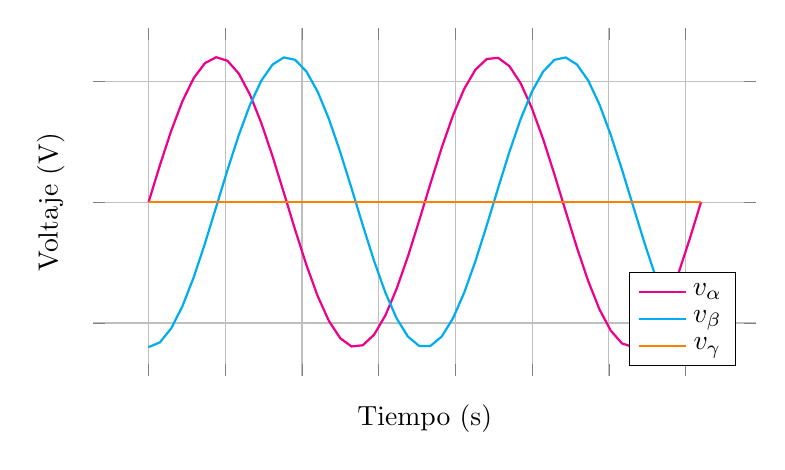
\begin{tikzpicture}
		\begin{axis}[
			width=10cm,
			height=6cm,
			xlabel={Tiempo (s)},
			ylabel={Voltaje (V)},
			legend entries={$v_{\alpha}$, $v_{\beta}$, $v_{\gamma}$},
			grid=major,  
			legend pos=south east,
			samples=50,
			domain=0:2*360,
			axis line style={draw=none},  % Elimina el recuadro exterior
			xticklabels=\empty,  % Elimina las marcas en el eje x
			yticklabels=\empty,  % Elimina las marcas en el eje y
			]
		
			\addplot[magenta, thick, domain=0:2*360] {1.2*sin(x)};
			\addplot[cyan, thick, domain=0:2*360] {1.2*sin(x - 90)};
			\addplot[orange, thick, domain=0:2*360] {0};
		\end{axis}
	\end{tikzpicture}
	\caption{Transformada de Clarke ortonormal representada en el tiempo.}
\end{figure}



No se derivará la transformada aquí, aunque es necesario comprender lo que hace y conocer la matriz de transformación.

Lo que hace la transformada es colocar dos de los ejes del sistema de referencia en el plano formado por el círculo generado por el vector espacial. El eje restante es perpendicular a ese plano y representa el componente homopolar.

A continuación se presenta la forma matricial de la transformada:

\begin{equation}
    \begin{bmatrix}
        \alpha \\
        \beta \\
        \gamma
    \end{bmatrix}
    =
    \sqrt{\frac{2}{3}}
    \begin{bmatrix}
        1 & -\frac{1}{2} & -\frac{1}{2} \\
        0 & \frac{\sqrt{3}}{2} & -\frac{\sqrt{3}}{2} \\
        \frac{1}{\sqrt{2}} & \frac{1}{\sqrt{2}} & \frac{1}{\sqrt{2}}
    \end{bmatrix}
    \begin{bmatrix}
        a \\
        b \\
        c
    \end{bmatrix}
\end{equation}

La forma matricial de la transformada inversa es:

\begin{equation}
    \begin{bmatrix}
        a \\
        b \\
        c
    \end{bmatrix}
    =
    \sqrt{\frac{2}{3}}
    \begin{bmatrix}
        1 & 0 & \frac{1}{\sqrt{2}} \\
        -\frac{1}{2} & \frac{\sqrt{3}}{2} & \frac{1}{\sqrt{2}} \\
        -\frac{1}{2} & -\frac{\sqrt{3}}{2} & \frac{1}{\sqrt{2}}
    \end{bmatrix}
    \begin{bmatrix}
        \alpha \\
        \beta \\
        \gamma
    \end{bmatrix}
\end{equation}

Esta transformada tiene la particularidad de mantener constante la potencia del sistema, de modo que se cumple la siguiente condición:

\begin{equation}
p(t) = p_{abc} = p_{\alpha\beta\gamma, \text{ortonormal}} = v_a \cdot i_a + v_b \cdot i_b + v_c \cdot i_c = v_\alpha \cdot i_\alpha + v_\beta \cdot i_\beta + v_\gamma \cdot i_\gamma
\end{equation}

\subsubsection{Transformada de Clarke de Amplitud Constante}

Mantener constante la potencia a lo largo de las transformadas puede ser útil en algunos contextos, pero lo que se suele implementar es una variante de la transformada de Clarke que mantiene constante la amplitud de la magnitud.

La transformada no es ortonormal, ya que ajusta las magnitudes para que el módulo de las variables sea el adecuado, pero la rotación se mantiene igual. A continuación se muestran la representación en el Espacio Vectorial y en un eje temporal:
\begin{figure}[H]
	\centering
	\hspace*{-1.5cm}
	\begin{tikzpicture}
		\begin{axis}[
			view={-45}{-35},
			%view={-20}{-15},
			%view={54.74}{-15},
			axis lines=none,  % Elimina los ejes
			xmin=-.9,
			xmax=.9,
			ymin=-.9,
			ymax=.9,
			zmin=-.9,
			zmax=.9,
			no markers,
			axis equal,
			enlargelimits={upper=0.2},
			scale=1,
			]
			\addplot3+[red, thick, no markers, samples=30, domain=-pi:pi, variable=\t]
			({sin(deg(\t))}, {sin(deg(\t + 2*pi/3))}, {sin(deg(\t - 2*pi/3))});
			
			% Ejes abc
			\draw[red, line width=1.5pt, -{Latex[length=1.5mm,width=1mm]}] (axis cs:0, 0, 0) -- (axis cs:0.5, 0, 0) node[pos=1.5]{$b$};
			\draw[red, line width=1.5pt, -{Latex[length=1.5mm,width=1mm]}] (axis cs:0, 0, 0) -- (axis cs:0, 0.5, 0) node[pos=1.5]{$a$};
			\draw[red, line width=1.5pt, -{Latex[length=1.5mm,width=1mm]}] (axis cs:0, 0, 0) -- (axis cs:0, 0, 0.5) node[pos=1.5]{$c$};
			
			% Ejes alpha-beta
			\draw[blue, line width=0.5pt, -{Latex[length=1.5mm,width=1mm]}] (axis cs:0, 0, 0) -- (axis cs:0, 0.5, 0) node[pos=1.5]{$\alpha'$};
			\draw[blue, line width=0.5pt, -{Latex[length=1.5mm,width=1mm]}] (axis cs:0, 0, 0) -- (axis cs:0.8, 0.6, 0.25) node[pos=1.5]{$\beta'$};
			
			\addplot3[draw=gray, no markers] coordinates {(-1.1, -1.1, -1.1) (-1.1, 1.1, -1.1)};
			\addplot3[draw=gray, no markers] coordinates {(-1.1, 1.1, -1.1) (1.1, 1.1, -1.1)};
			\addplot3[draw=gray, no markers] coordinates {(1.1, 1.1, -1.1) (1.1, -1.1, -1.1)};
			\addplot3[draw=gray, no markers] coordinates {(1.1, -1.1, -1.1) (-1.1, -1.1, -1.1)};
			\addplot3[draw=gray, no markers] coordinates {(-1.1, -1.1, 1.1) (-1.1, 1.1, 1.1)};
			\addplot3[draw=gray, no markers] coordinates {(-1.1, 1.1, 1.1) (1.1, 1.1, 1.1)};
			\addplot3[draw=gray, no markers] coordinates {(1.1, 1.1, 1.1) (1.1, -1.1, 1.1)};
			\addplot3[draw=gray, no markers] coordinates {(1.1, -1.1, 1.1) (-1.1, -1.1, 1.1)};
			\addplot3[draw=gray, no markers] coordinates {(-1.1, -1.1, -1.1) (-1.1, -1.1, 1.1)};
			\addplot3[draw=gray, no markers] coordinates {(-1.1, 1.1, -1.1) (-1.1, 1.1, 1.1)};
			\addplot3[draw=gray, no markers] coordinates {(1.1, 1.1, -1.1) (1.1, 1.1, 1.1)};
			\addplot3[draw=gray, no markers] coordinates {(1.1, -1.1, -1.1) (1.1, -1.1, 1.1)};
		\end{axis}
	\end{tikzpicture}
	\centering
	\caption{Sistema trifásico representado en el Espacio Vectorial con la transformada de Clarke de amplitud constante superpuesta.}
\end{figure}

\begin{figure}[H]
	\centering
	\hspace*{-1.5cm}
	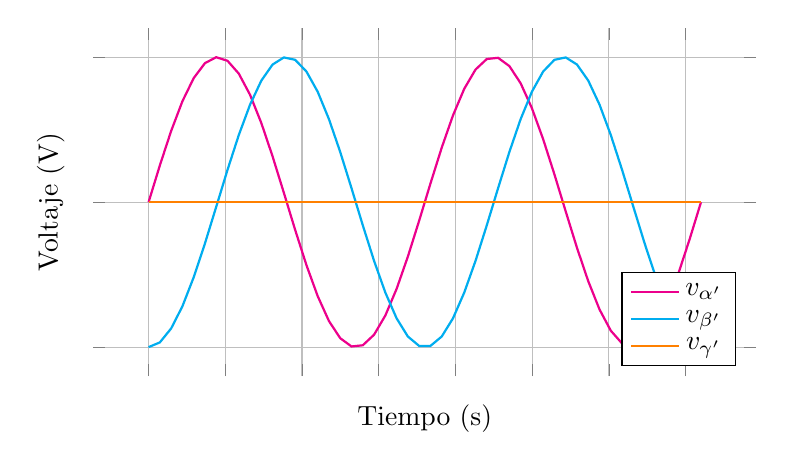
\begin{tikzpicture}
		\begin{axis}[
			width=10cm,
			height=6cm,
			xlabel={Tiempo (s)},
			ylabel={Voltaje (V)},
			legend entries={$v_{\alpha'}$, $v_{\beta'}$, $v_{\gamma'}$},
			grid=major,  
			legend pos=south east,
			samples=50,
			domain=0:2*360,
			axis line style={draw=none},  % Elimina el recuadro exterior
			xticklabels=\empty,  % Elimina las marcas en el eje x
			yticklabels=\empty,  % Elimina las marcas en el eje y
			]
			
			\addplot[magenta, thick, domain=0:2*360] {sin(x)};
			\addplot[cyan, thick, domain=0:2*360] {sin(x - 90)};
			\addplot[orange, thick, domain=0:2*360] {0};
		\end{axis}
	\end{tikzpicture}
	\caption{Transformada de Clarke de amplitud constante representada en el tiempo.}
\end{figure}

\begin{equation}
    \begin{bmatrix}
        \alpha' \\
        \beta' \\
        \gamma'
    \end{bmatrix}
    =
    \frac{2}{3}
    \begin{bmatrix}
        1 & -\frac{1}{2} & -\frac{1}{2} \\
        0 & \frac{\sqrt{3}}{2} & -\frac{\sqrt{3}}{2} \\
        \frac{1}{2} & \frac{1}{2} & \frac{1}{2}
    \end{bmatrix}
    \begin{bmatrix}
        a \\
        b \\
        c
    \end{bmatrix}
\end{equation}

La transformada inversa es la siguiente:

\begin{equation}
    \begin{bmatrix}
        a \\
        b \\
        c
    \end{bmatrix}
    =
    \begin{bmatrix}
        1 & 0 & 1 \\
        -\frac{1}{2} & \frac{\sqrt{3}}{2} & 1 \\
        -\frac{1}{2} & -\frac{\sqrt{3}}{2} & 1
    \end{bmatrix}
    \begin{bmatrix}
        \alpha' \\
        \beta' \\
        \gamma'
    \end{bmatrix}
\end{equation}

Se puede derivar que:

\begin{equation}
p_{abc} = \frac{3}{2} \cdot (v_{\alpha'} \cdot i_{\alpha'} + v_{\beta'} \cdot i_{\beta'} + v_{\gamma'} \cdot i_{\gamma'})
\end{equation}


\subsubsection{Transformada de Park}

Después de aplicar la transformada de Clarke, todavía quedan dos variables sinusoidales (\(\alpha\beta\) si se considera \(\gamma = 0\)), lo que dificulta el análisis para que el control sea sencillo. Por lo tanto, se aplica otra transformada para convertir estas cantidades sinusoidales en constantes.

Ahora, considerando que el vector espacial gira a una velocidad de \(\omega = 2\pi f\), si se aplica continuamente una rotación alrededor del eje \(\gamma\) con un ángulo \(\theta = \omega  t\), se puede representar el vector espacial como una composición de dos variables continuas (en lugar de sinusoides). Además, si se sincroniza esta rotación con el ángulo del vector espacial (el eje \(d\) apuntando al vector espacial), se obtiene una variable continua (\(q\)) y una segunda variable de valor nulo (\(d\)).

\begin{figure}[H]
  	\centering
  \hspace*{-1.5cm}
  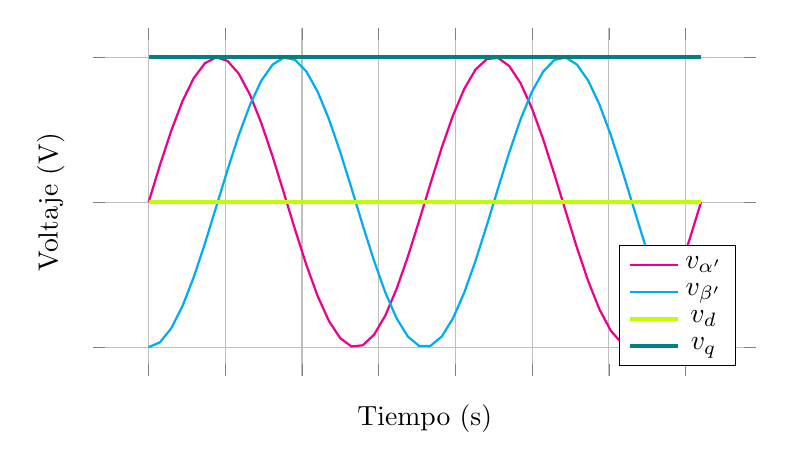
\begin{tikzpicture}
  	\begin{axis}[
  		width=10cm,
  		height=6cm,
  		xlabel={Tiempo (s)},
  		ylabel={Voltaje (V)},
  		legend entries={$v_{\alpha'}$, $v_{\beta'}$, $v_d$, $v_q$},
  		grid=major,  
  		legend pos=south east,
  		samples=50,
  		domain=0:2*360,
  		axis line style={draw=none},  % Elimina el recuadro exterior
  		xticklabels=\empty,  % Elimina las marcas en el eje x
  		yticklabels=\empty,  % Elimina las marcas en el eje y
  		]
  		
  		\addplot[magenta, thick, domain=0:2*360] {sin(x)};
  		\addplot[cyan, thick, domain=0:2*360] {sin(x - 90)};
  		
  		\addplot[lime, ultra thick, domain=0:2*360] {0};
  		\addplot[teal, ultra thick, domain=0:2*360] {1};
  		
  		
  	\end{axis}
  \end{tikzpicture}
  \caption{Transformada de Park representada en el tiempo junto a la transformada de Clarke de amplitud constante.}
\end{figure}

Se puede ver que la transformada es simplemente una rotación a lo largo de uno de los ejes de la base:

\begin{equation}
    \begin{bmatrix}
        d \\
        q \\
        0
    \end{bmatrix}
    =
    \begin{bmatrix}
        \cos(\theta) & \sin(\theta) & 0 \\
        -\sin(\theta) & \cos(\theta) & 0 \\
        0 & 0 & 1
    \end{bmatrix}
    \begin{bmatrix}
        \alpha \\
        \beta \\
        \gamma
    \end{bmatrix}
\end{equation}

\subsection{Marco de referencia rotatorio}

En esta sección, se convertirá el modelo trifásico inicial del PMSM en un modelo continuo en el marco de referencia $d - q$. Antes, se omitieron las ecuaciones del modelo trifásico, pero utilizando estas y aplicando las transformadas de Clarke y Park, se obtienen las ecuaciones que se derivarán en esta sección.

El enfoque general es utilizar la transformada de amplitud constante, lo que lleva a estas ecuaciones para las tensiones y corrientes del estator:

\begin{equation}
	\begin{bmatrix}
		v_d \\
		v_q \\
		v_0
	\end{bmatrix}
	=
	\begin{bmatrix}
		\cos(\theta) & \sin(\theta) & 0  \\
		-\sin(\theta) & \cos(\theta) & 0  \\
		0 & 0 & 1
	\end{bmatrix}
	\frac{2}{3}
	\begin{bmatrix}
		1 & -\frac{1}{2} & -\frac{1}{2} \\
		0 & \frac{\sqrt{3}}{2} & -\frac{\sqrt{3}}{2} \\
		\frac{1}{2} & \frac{1}{2} & \frac{1}{2}
	\end{bmatrix}
	\begin{bmatrix}
		v_a \\
		v_b \\
		v_c
	\end{bmatrix}
\end{equation}

\begin{equation}
	\begin{bmatrix}
		i_d \\
		i_q \\
		i_0
	\end{bmatrix}
	=
	\begin{bmatrix}
		\cos(\theta) & \sin(\theta) & 0  \\
		-\sin(\theta) & \cos(\theta) & 0  \\
		0 & 0 & 1
	\end{bmatrix}
	\frac{2}{3}
	\begin{bmatrix}
		1 & -\frac{1}{2} & -\frac{1}{2} \\
		0 & \frac{\sqrt{3}}{2} & -\frac{\sqrt{3}}{2} \\
		\frac{1}{2} & \frac{1}{2} & \frac{1}{2}
	\end{bmatrix}
	\begin{bmatrix}
		i_a \\
		i_b \\
		i_c
	\end{bmatrix}
\end{equation}

El modelo de circuito equivalente se divide en los circuitos del eje $d$ y el eje $q$:


\begin{figure}[H]
	\centering
	\begin{minipage}{0.45\textwidth}
		\centering
		\begin{circuitikz}[american voltages]
			% d-axis circuit
			\draw (0,0) to [L, l=$L_d$, o-] ++(2,0) to [R, l=$R_s$] ++(2,0) to [V, v^=$\omega_e\cdot L_q\cdot i_q$, invert] ++(2,0) -- ++(0,-2){};
			% Parallel line
			\draw (0,-2) node[circ, fill=none]{} -- ++(6,0);
			% Current label
			\draw (4,-2) to [open, i_=$i_d$] (2,-2);
			% Voltage labels
			\draw (0,0) to [open, v^=$v_d$] (0,-2);
		\end{circuitikz}
	\end{minipage}
	\hspace{0.05\textwidth}
	\begin{minipage}{0.45\textwidth}
		\centering
		\begin{circuitikz}[american voltages]
			% q-axis circuit
			\draw (0,0) to [L, l=$L_q$, o-] ++(2,0) to [R, l=$R_s$] ++(2,0) to [V, v^=$\omega_e\cdot L_d\cdot i_d$] ++(2,0) to [V, v^=$\omega_e\cdot\lambda_m$] ++(0,-2){};
			% Parallel line
			\draw (0,-2) node[circ, fill=none]{} -- ++(6,0);
			% Current label
			\draw (4,-2) to [open, i_=$i_q$] (2,-2);
			% Voltage labels
			\draw (0,0) to [open, v^=$v_q$] (0,-2);
		\end{circuitikz}
	\end{minipage}
	\caption{Circuitos eléctricos equivalentes del modelo $d-q$ de un PMSM.}
\end{figure}

Se puede observar que:

\begin{equation}
v_d = v_{R_s} - \omega_e \cdot L_q \cdot i_q + v_{L_d}
\end{equation}

\begin{equation}
v_d = R_s\cdot i_d - \omega_e \cdot L_q \cdot i_q + L_d\cdot\frac{d i_d}{d t}
\end{equation}

Y:

\begin{equation}
v_q = v_{R_s} - \omega_e \cdot L_d \cdot i_d + \omega_e \cdot \lambda_m + v_{L_q}
\end{equation}

\begin{equation}
v_q = R_s\cdot i_q - \omega_e \cdot L_d \cdot i_q + \omega_e \cdot \lambda_m + L_q\cdot\frac{d i_q}{d t}
\end{equation}

En estado estacionario, es decir, sin cambios muy bruscos de la corriente, el término diferencial puede ser eliminado:

\begin{equation}
	v_d = R_s\cdot i_d - \omega_e \cdot L_q \cdot i_q
	\label{eq_vd}
\end{equation}
\begin{equation}
	v_q = R_s\cdot i_q - \omega_e \cdot L_d \cdot i_q + \omega_e \cdot \lambda_m
	\label{eq_vq}
\end{equation}


Donde:
\begin{itemize}
    \item \(v_d\) y \(v_q\) son las tensiones en los ejes d y q respectivamente.
    \item \(i_d\) y \(i_q\) son las corrientes en los ejes d y q respectivamente.
    \item \(L_d\) y \(L_q\) son las inductancias en los ejes d y q respectivamente.
    \item \(\omega_e\) es la velocidad eléctrica, que es la velocidad mecánica multiplicada por el número de pares de polos del PMSM (\(\omega_e = \omega_m \cdot pp = \omega_m \cdot \frac{n}{2}\)).
    \item \(\lambda_m\) es el flujo magnético generado por los imanes permanentes. La magnitud del flujo magnético generado afecta directamente la magnitud de la tensión inducida en las fases del estator. Este parámetro se puede transformar fácilmente en \(k_E\), que es la relación entre la velocidad mecánica del rotor y la tensión generada en las 3 fases.
\end{itemize}


Hay PMSM cuyos imanes están montados dentro del rotor (IPM) y otros cuyos imanes están en la superficie del rotor (SPM). Esta diferenciación juega un papel importante en el desarrollo del modelo y el control, porque en los SPM se cumple \(L_d = L_q\), a menudo escrito solo como \(L\). Además, si se trata de un IPM, la orientación de los imanes puede cambiar las trayectorias del control, de manera que si son imanes tangenciales se da \(L_d > L_q\) y si son imanes radiales \(L_d < L_q\). Se desarrollarán las ecuaciones para motores IPM con imanes radiales, pero se ha de tener en cuenta que se pueden realizar muchas simplificaciones si el motor es un SPM. Una situación que se dará es que algunas ecuaciones tienen alguna forma de \(L_d - L_q\) como denominador, lo cual es bastante problemático si se está tratando de implementar la ecuación directamente. Por ese motivo, es mejor diferenciar el tipo de motor antes de implementar las ecuaciones. Una solución válida es tener en cuenta la anisotropía magnética que suelen presentar la mayoría de SPMs, con lo que \(L_d < L_q\) y se pueden aplicar las ecuaciones del IPM a costa de potencia de cálculo, de ejecutarse el control en tiempo real.

\begin{figure}[H]
	\centering
	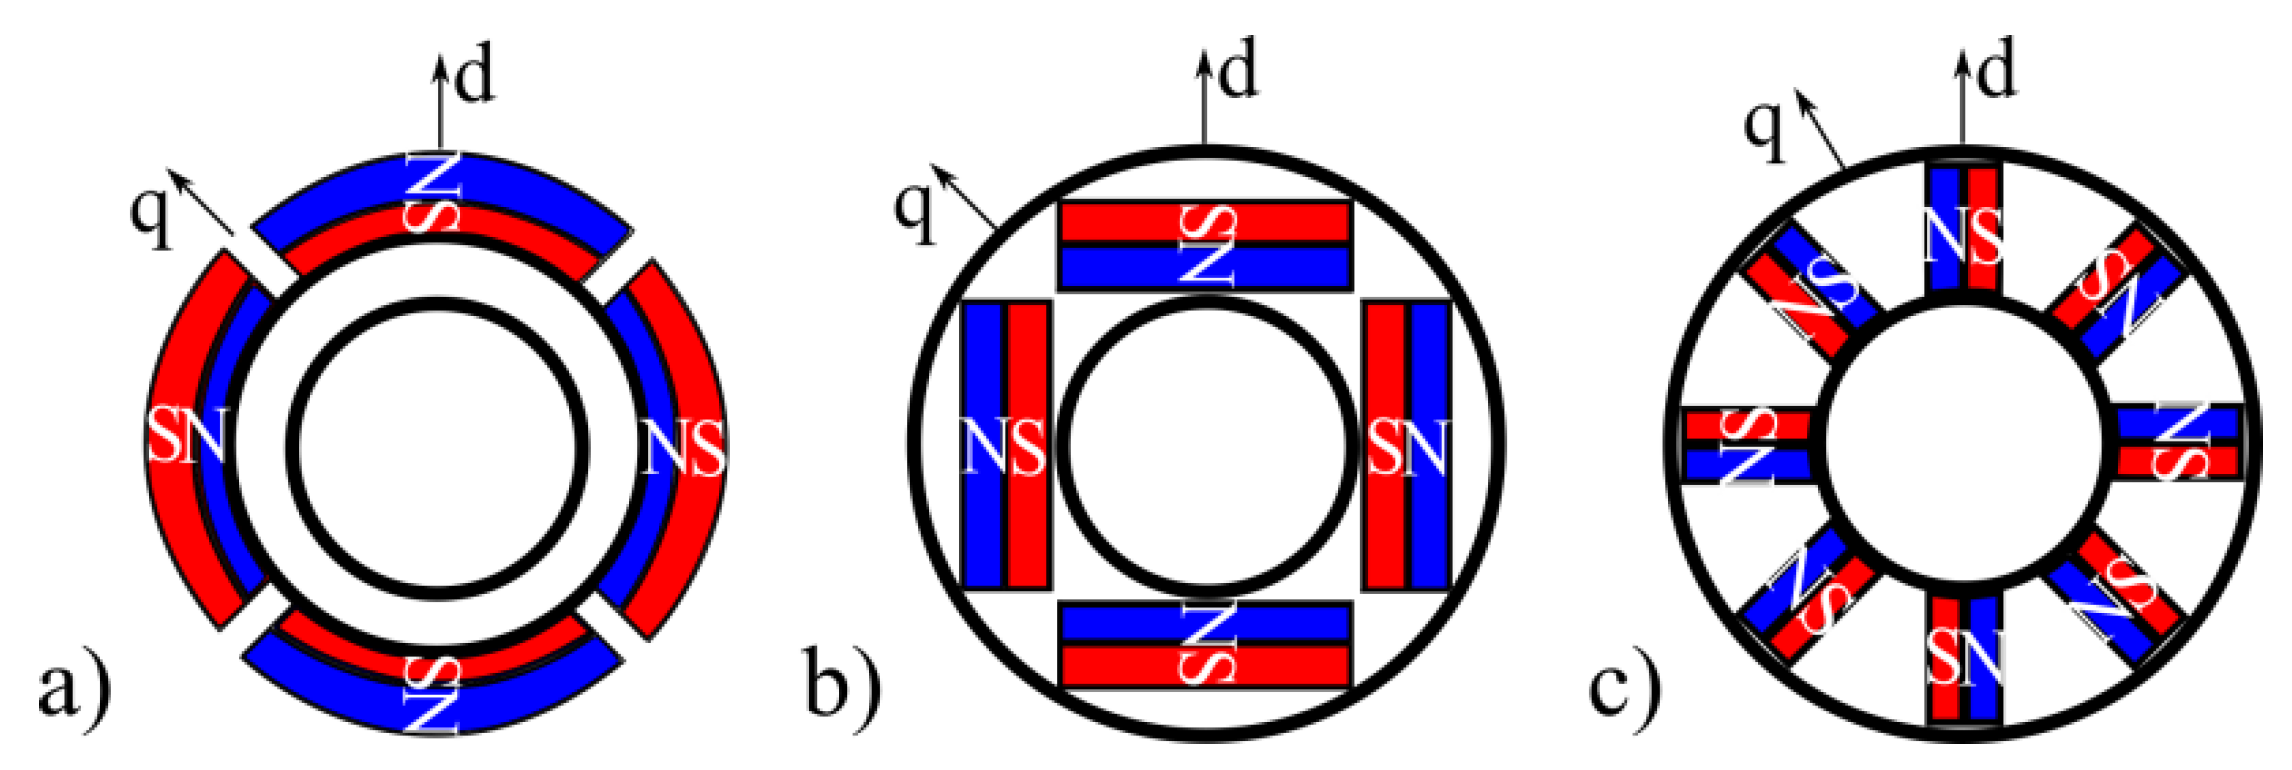
\includegraphics[width=0.7\linewidth]{fig/motor-types}
	\caption{Tipos de PMSMs según la disposición de los imanes. a) SPM, b) IPM radial, c) IPM tangencial.}
\end{figure}


La potencia eléctrica se define como:

\begin{equation}
p_e = \frac{3}{2}\cdot(v_d i_d + v_q i_q)
\end{equation}

Si se supone que la máquina es perfectamente eficiente, se puede decir que la potencia mecánica es igual a la potencia eléctrica, \(p_e = p_m\). Sabiendo que \(p_m = \omega_m T_{em}\), donde \(T_{em}\) es el par electromagnético producido, se puede derivar:

\begin{equation}
T_{em} = \frac{3}{2\cdot \omega_m}\cdot(v_d i_d + v_q i_q) = \frac{3}{2\cdot \omega_e}\frac{n}{2}\cdot(v_d i_d + v_q i_q)
\end{equation}

\begin{equation}
T_{em} = \frac{3}{2}\frac{n}{2}\cdot((L_d - L_q) i_q i_d + \lambda_m i_q)
\label{eq_tq_dq}
\end{equation}

También se puede establecer un límite de voltaje, porque el PMSM generalmente se controla con un inversor de fuente de voltaje (VSI) modulado por SVPWM y la tensión de salida $V_s$ está limitada a \(\frac{V_{DC}}{\sqrt{3}}\). En esta ecuación, no se considera la caída de tensión por la resistencia del estator \(R_s\), ya que haría que las ecuaciones fueran muy densas y el efecto de esta caída de voltaje es despreciable a altas velocidades.

\begin{equation}
V_s = \sqrt{v_d^2 + v_q^2} \leq \frac{V_{DC}}{\sqrt{3}}
\end{equation}
\begin{equation}
	\sqrt{\left(R_s\cdot i_d - \omega_e \cdot L_q \cdot i_q\right)^2 + \left(R_s\cdot i_q - \omega_e \cdot L_d \cdot i_q + \omega_e \cdot \lambda_m\right)^2} \leq \frac{V_{DC}}{\sqrt{3}}
\end{equation}

Despreciando los términos con \(R_s\):
\begin{equation}
	\sqrt{\left(- \omega_e \cdot L_q \cdot i_q\right)^2 + \left(- \omega_e \cdot L_d \cdot i_q + \omega_e \cdot \lambda_m\right)^2} \leq \frac{V_{DC}}{\sqrt{3}}
\end{equation}
 
Reordenando:
\begin{equation}
	\left(\frac{\frac{V_{DC}}{\sqrt{3}}}{\omega_e}\right)^2 \geq \left(\lambda_m+L_d\cdot i_d\right)^2+(L_q\cdot i_q)^2
	\label{eq_vle_dq}
\end{equation}

\subsection{Curvas características del PMSM}

Las ecuaciones del PMSM son muy útiles cuando se diseña el control y la implementación real, pero antes de eso, es muy recomendable verlas en un gráfico para comprender mejor algunas de las intuiciones detrás de ellas.

\subsubsection{Curva de par-velocidad y potencia-velocidad}

Las primeras curvas estudiadas son las de par-velocidad y potencia-velocidad. Definen la intención de diseño del PMSM, ilustrando el rendimiento deseado. El objetivo al diseñar el control es tratar de igualar o incluso superar estas curvas.


\begin{figure}[H]
    \centering
    \hspace*{-1.5cm}
    \begin{tikzpicture}
    \begin{axis}[
        axis lines=middle,
        width=10cm,
        height=8cm,
        x label style={at={(axis description cs:-0.1,0.5)},anchor=north},
        y label style={at={(axis description cs:0.5,-0.1)},rotate=90,anchor=south},
        xlabel={$\omega_m$},
        ylabel={$T_{em}$},
        ytick={-26, 26},
        xtick={-2000,-1000,1000,2000},
        yticklabels={$-T_{em,max}$, $T_{em,max}$},
        xticklabels={$-\omega_{m,max}$, $-\omega_{m,nom}$, $\omega_{m,nom}$,$\omega_{m,max}$},
        grid=none,  
        ymin=-40,
        ymax=40,
        samples=15,
        domain=-2500:2500,
        nodes near coords align={south east},
        y tick label style={yshift={sign(\tick)*10}},
        ylabel style={rotate=-90},
        %no marks
        % axis line style={draw=none},  % Elimina el recuadro exterior
    ]
    \addplot[blue, thick, domain=-1000:1000] {26};
    \addplot[blue, thick, domain=-1000:1000] {-26};
    \addplot[blue, thick, domain=1000:2500] {26000/x};
    \addplot[blue, thick, domain=-2500:-1000] {-26000/x};
    \addplot[white, line width=1mm, domain=2000:2500] {26000/x};
    \addplot[white, line width=1mm, domain=-2500:-2000] {-26000/x};
    \addplot[blue, thick, domain=1000:2500] {-26000/x};
    \addplot[blue, thick, domain=-2500:-1000] {26000/x};
    \addplot[white, line width=1mm, domain=2000:2500] {-26000/x};
    \addplot[white, line width=1mm, domain=-2500:-2000] {26000/x};
    \end{axis}
    \end{tikzpicture}
    \caption{Curva de par-velocidad del PMSM.}
\end{figure}


La curva es una función por tramos, que toma \(T_{em,max}\), \(\omega_{m,max}\) y \(P_{m,max}\) como sus parámetros.

La curva es constante desde \(\omega_m = 0\) hasta \(\omega_m = \omega_{m,nom} = \frac{P_{m,max}}{T_{em,max}}\), donde su valor es \(T_{em,max}\). Esta porción es lo que se conoce como la zona de par constante. Desde \(\omega_m = \omega_{m,nom}\) hasta \(\omega_m = \omega_{m,max}\), \(T_{em}\) se define como \(T_{em} = \frac{P_{m,max}}{\omega_m}\), lo que da una curva de tipo \(y=\frac{a}{x}\). Esto se llama la zona de potencia constante.

\[
T_{em} = 
\begin{cases}
  T_{em,max} & -\omega_{m,nom} < \omega_m < \omega_{m,nom} \\
  -T_{em,max} & -\omega_{m,nom} < \omega_m < \omega_{m,nom} \\
  \frac{P_{m,max}}{\omega_m} & \omega_{m,nom}\leq \omega_m\leq \omega_{m,max} (T_{em,max}),-\omega_{m,max}\leq \omega_m\leq -\omega_{m,nom} (-T_{em,max})\\
  -\frac{P_{m,max}}{\omega_m} & \omega_{m,nom}\leq \omega_m\leq \omega_{m,max} (-T_{em,max}),-\omega_{m,max}\leq \omega_m\leq -\omega_{m,nom} (T_{em,max})
\end{cases}
\]

Además \(P_m\) aumentará linealmente con \(\omega_m\) hasta \(\omega_{m,nom}\), ya que \(P_m = T_{em} \cdot \omega_m\). Desde \(\omega_{m,nom}\) hasta \(\omega_{m,max}\), \(P_m\) es una recta de valor \(P_{m,max}\)

\begin{figure}[H]
	\centering
	\hspace*{-1.5cm}
	\begin{tikzpicture}
		\begin{axis}[
			axis lines=middle,
			width=10cm,
			height=8cm,
			x label style={at={(axis description cs:-0.1,0.5)},anchor=north},
			y label style={at={(axis description cs:0.5,-0.1)},rotate=90,anchor=south},
			xlabel={$\omega_m$},
			ylabel={$P_{em}$},
			ytick={-26, 26},
			xtick={-2000,-1000,1000,2000},
			yticklabels={$-P_{m,max}$, $P_{m,max}$},
			xticklabels={$-\omega_{m,max}$, $-\omega_{m,nom}$, $\omega_{m,nom}$,$\omega_{m,max}$},
			grid=none,  
			ymin=-40,
			ymax=40,
			samples=15,
			domain=-2500:2500,
			nodes near coords align={south east},
			y tick label style={yshift={sign(\tick)*10}},
			ylabel style={rotate=-90},
			%no marks
			% axis line style={draw=none},  % Elimina el recuadro exterior
			]
			\addplot[blue, thick, domain=-1000:1000] {x*26/1000};
			\addplot[blue, thick, domain=-1000:1000] {-x*26/1000};
			\addplot[blue, thick, domain=1000:2500] {26};
			\addplot[blue, thick, domain=-2500:-1000] {-26};
			\addplot[white, line width=1mm, domain=2000:2500] {26};
			\addplot[white, line width=1mm, domain=-2500:-2000] {-26};
			\addplot[blue, thick, domain=1000:2500] {-26};
			\addplot[blue, thick, domain=-2500:-1000] {26};
			\addplot[white, line width=1mm, domain=2000:2500] {-26};
			\addplot[white, line width=1mm, domain=-2500:-2000] {26};
		\end{axis}
	\end{tikzpicture}
	\caption{Curva de potencia-velocidad del PMSM.}
\end{figure}


\subsubsection{CLC (Círculo de límite de corriente)}

Es obvio que la corriente eléctrica suministrada al PMSM debe estar limitada. Por lo general, el fabricante del motor establecerá la corriente alterna máxima, lo cual se traduce en un límite para \(i_d\) y \(i_q\).

A continuación, se presenta un gráfico muy útil para conocer los límites del motor. Se establecen los ejes como $i_d$ e $i_q$. Por ejemplo, si un motor está funcionando con $i_d = -1 \text{A}$ e $i_q = 5 \text{A}$, se dibuja un punto en $(-1,5)$. Como se puede apreciar, este es un sistema de coordenadas cartesianas. También puede convertirse en un sistema de coordenadas polares, que utiliza una magnitud y un ángulo. La magnitud del vector será entonces:
\begin{equation}
I_{s} = \sqrt{i_d^2+i_q^2} [\text{A}]
\end{equation}

Y el ángulo:

\begin{equation}
\gamma = \arctan\left(\frac{i_q}{i_d}\right) [\text{rad}]
\end{equation}

Se puede observar que la corriente máxima puede expresarse más fácilmente como $I_s$, independientemente del ángulo $\gamma$ (no debe confundirse con el $\gamma$ de la transformada de Clarke). Por lo tanto, se puede representar $I_s = I_{s,\text{max}} , \forall \gamma \in [0,2\pi]$

\begin{figure}[H]
	\centering
	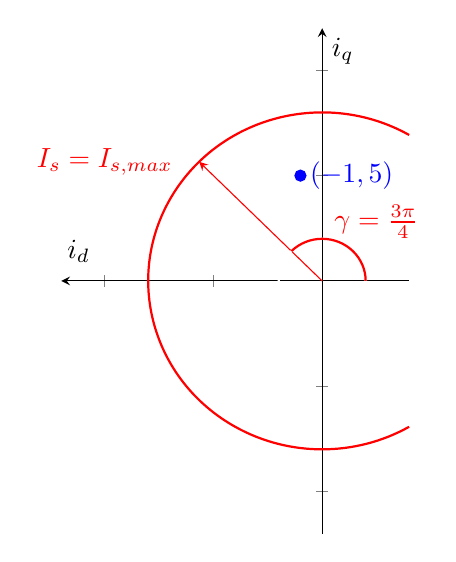
\begin{tikzpicture}
		\begin{axis}[
			axis lines=middle,
			width=6cm,
			height=8cm,
			xlabel={$i_d$},
			x label style={at={(axis description cs:0.05,0.6)},anchor=north},
			ylabel={$i_q$},
			grid=none,
			xmin=-1.2,
			xmax=0.4,
			ymin=-1.2,
			ymax=1.2,
			no markers,
			x axis line style={stealth-},
			xticklabels=\empty,
			yticklabels=\empty,
			clip=false,          % Disable clipping
			]
			
			% Límite de corriente Is_max
			\draw [red, thick] (0.4,0.693) arc (60:300:0.8);
			\draw [red, -stealth](0,0) -- (-0.56568542494,0.56568542494) node at (-1,0.56568542494) {$I_s = I_{s,\text{max}}$};
			\draw [white, thick] (axis cs: 0.2, 0) arc (0:180:0.2);
			\draw [red, thick] (axis cs: 0.2, 0) arc (0:135:0.2);
			\node [red] at (axis cs: 0.25, 0.28) {$\gamma = \frac{3\pi}{4}$};
			
			% Added point (-0.1, 0.5)
			\filldraw[blue] (-0.1, 0.5) circle (2pt) node[anchor=west] {$(-1, 5)$};
			
		\end{axis}
	\end{tikzpicture}
	\caption{Círculo de límite de corriente con punto añadido.}
\end{figure}



Resulta ser un círculo, lo cual tiene sentido, ya que es un vector de magnitud constante. Además, el vector de corriente $I_s\angle \gamma = I_{s,\text{max}} \angle{\frac{3\pi}{4}}$ se representa para facilitar su comprensión.


\subsubsection{TH (Hipérbolas de par)}

Si se estudia la ecuación del par \ref{eq_tq_dq}, es evidente que \(T_{em}\) es una función de \((i_d, i_q)\). El resto de parámetros son constantes, por lo que se puede establecer un valor fijo de par y deslizar alrededor de \((i_d, i_q)\) para generar una curva. La forma de la curva resultante es una hipérbola, y a continuación se presenta en su forma polar:

\begin{equation}
T_{em} = \frac{3}{2}pp\cdot((L_d - L_q)\cdot I_s^2 \cdot \sin(\gamma)\cos(\gamma) + \lambda_m\cdot I_s\cdot \sin(\gamma))
\label{eq_tq_pol}
\end{equation}




\begin{figure}[H]
  \centering
    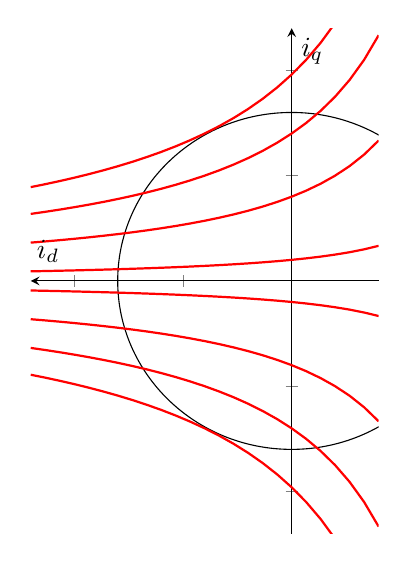
\begin{tikzpicture}
    \begin{axis}[
        axis lines=middle,
        width=6cm,
        height=8cm,
        xlabel={$i_d$},
        x label style={at={(axis description cs:0.05,0.6)},anchor=north},
        ylabel={$i_q$},
        %y label style={at={(axis description cs:0.95,0.05}},
        grid=none,
        xmin=-1.2,
        xmax=0.4,
        ymin=-1.2,
        ymax=1.2,
        no markers,
        x axis line style = {stealth-},
        xticklabels=\empty,  % Elimina las marcas en el eje x
        yticklabels=\empty,  % Elimina las marcas en el eje y
    ]
    
    \draw[black] (0,0) circle [radius=0.8];
    \addplot[red, thick, domain=-1.2:0.4] {4*0.1/(3*2*((2/3)+(2/3)/1*(1-2)*x))};
    \addplot[red, thick, domain=-1.2:0.4] {4*0.4/(3*2*((2/3)+(2/3)/1*(1-2)*x))};
    \addplot[red, thick, domain=-1.2:0.4] {4*0.7/(3*2*((2/3)+(2/3)/1*(1-2)*x))};
    \addplot[red, thick, domain=-1.2:0.4] {4*0.98/(3*2*((2/3)+(2/3)/1*(1-2)*x))};
    
    \addplot[red, thick, domain=-1.2:0.4] {-4*0.1/(3*2*((2/3)+(2/3)/1*(1-2)*x))};
    \addplot[red, thick, domain=-1.2:0.4] {-4*0.4/(3*2*((2/3)+(2/3)/1*(1-2)*x))};
    \addplot[red, thick, domain=-1.2:0.4] {-4*0.7/(3*2*((2/3)+(2/3)/1*(1-2)*x))};
    \addplot[red, thick, domain=-1.2:0.4] {-4*0.98/(3*2*((2/3)+(2/3)/1*(1-2)*x))};
    

    \end{axis}
    \end{tikzpicture}
  \caption{Hipérbolas de par.}
\end{figure}


El gráfico se limita a los cuadrantes 2 y 3 por un motivo ilustrado con estas hipérbolas: solo los valores negativos de \(i_d\) contribuyen a la generación de par. Cuando \(i_d>0\), se necesita más corriente para generar la misma cantidad de par. Cuanto más alejada está la hipérbole del eje \(i_d\), más par representa en valor absoluto. Aquellas hipérbolas que quedan por encima del eje \(i_d\), es decir, \(i_q > 0\) son par positivo, mientras que si \(i_q < 0\), el par es de sentido opuesto.

\subsubsection{VLE (Elipses de límite de voltaje)}

Tomando la ecuación de voltaje \ref{eq_vle_dq}, se puede demostrar que es una elipse. Del mismo modo que con las hipérbolas de par, se pueden establecer una velocidad y una tensión, y deslizar valores de \((i_d, i_q)\) para generar la curva.

\begin{equation}
1 \geq \frac{\left(\frac{\lambda_m}{L_d}+i_d\right)^2}{\left(\frac{\frac{V_{DC}}{\sqrt{3}}}{L_d\omega_e}\right)^2}+\frac{i_q^2}{\left(\frac{\frac{V_{DC}}{\sqrt{3}}}{L_q\omega_e}\right)^2}
\end{equation}




\begin{figure}[H]
  \centering
    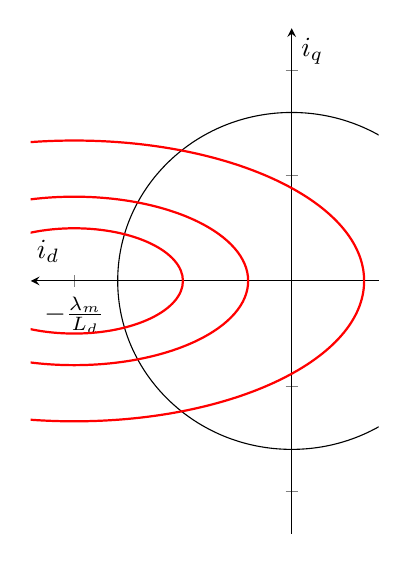
\begin{tikzpicture}
    \begin{axis}[
        axis lines=middle,
        width=6cm,
        height=8cm,
        xlabel={$i_d$},
        x label style={at={(axis description cs:0.05,0.6)},anchor=north},
        ylabel={$i_q$},
        %y label style={at={(axis description cs:0.95,0.05}},
        grid=none,
        xmin=-1.2,
        xmax=0.4,
        ymin=-1.2,
        ymax=1.2,
        no markers,
        x axis line style = {stealth-},
        xtick = {-1},
        xticklabels={$-\frac{\lambda_m}{L_d}$},  % Elimina las marcas en el eje x
        yticklabels=\empty,  % Elimina las marcas en el eje y
    ]
    
    
    \draw[black] (0,0) circle [radius=0.8];
    \draw[red, thick] (-1,0) ellipse (1.333333 and 0.66666666);
    \draw[red, thick] (-1,0) ellipse (0.8 and 0.4);
    \draw[red, thick] (-1,0) ellipse (0.5 and 0.25);

    \end{axis}
    \end{tikzpicture}
  \caption{Elipses de límite de voltaje con $I_{sc} > I_{s,max}$.}
\end{figure}


Al representar estas elipses, normalmente se anotan los valores de velocidad en rpm mecánicas, ya que es mucho más fácil hacerse una idea de los límites del motor junto al resto de curvas (\(\omega_m [\text{rpm}] = \frac{1}{pp} \omega_e \left[\frac{\text{rad}}{s}\right] \cdot \frac{60}{2\pi}\)).

Las elipses se reducen a medida que la velocidad aumenta. El foco de las elipses está ubicado exactamente en \((i_d, i_q)=(-I_{sc}, 0) = \left(-\frac{\lambda_m}{L_d},0\right)\). En el gráfico anterior, el foco está fuera del círculo de límite de corriente, pero no siempre es el caso. Si \(I_{sc} \leq I_{s,max}\), teóricamente el motor puede alcanzar una velocidad infinita, ya que las elipses colapsan en un solo punto. 



\begin{figure}[H]
  \centering
    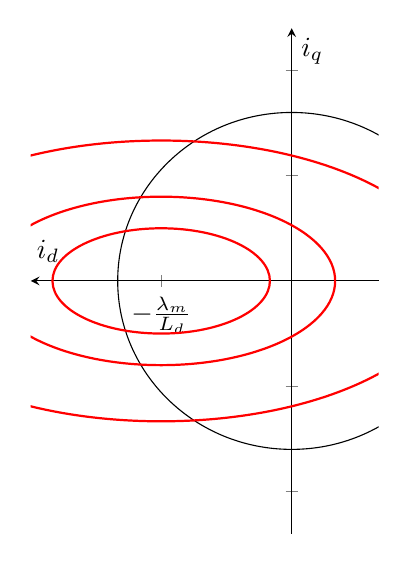
\begin{tikzpicture}
    \begin{axis}[
        axis lines=middle,
        width=6cm,
        height=8cm,
        xlabel={$i_d$},
        x label style={at={(axis description cs:0.05,0.6)},anchor=north},
        ylabel={$i_q$},
        %y label style={at={(axis description cs:0.95,0.05}},
        grid=none,
        xmin=-1.2,
        xmax=0.4,
        ymin=-1.2,
        ymax=1.2,
        no markers,
        x axis line style = {stealth-},
        xtick = {-0.6},
        xticklabels={$-\frac{\lambda_m}{L_d}$},  % Elimina las marcas en el eje x
        yticklabels=\empty,  % Elimina las marcas en el eje y
    ]
    
    
    \draw[black] (0,0) circle [radius=0.8];
    \draw[red, thick] (-0.6,0) ellipse (1.333333 and 0.66666666);
    \draw[red, thick] (-0.6,0) ellipse (0.8 and 0.4);
    \draw[red, thick] (-0.6,0) ellipse (0.5 and 0.25);

    \end{axis}
    \end{tikzpicture}
  \caption{Elipses de límite de voltaje con $I_{sc} \leq I_{s,max}$.}
\end{figure}




%% HASTA AQUI TRACUCCION POCHA DE LA WIKI

\section{Control del PMSM en el espacio d-q}
\subsection{Trayectorias de control}

Después de conocer los límites de la máquina, se pueden establecer criterios para decidir cuánto \(i_d\) y \(i_q\) (o \(I_s\) y \(\gamma\)) se deben aplicar al PMSM para que se comporte mecánicamente como se desee. El conjunto de puntos de trabajo que definen un comportamiento se llama trayectoria y existen una multitud de ellas. Por ejemplo, se puede desear que el motor produzca la mayor cantidad de par posible con la mínima corriente. Pero también se podría querer que tenga un cierto factor de potencia o que mantenga el par constante subiendo la velocidad, etc.

En un monoplaza de Formula Student, se desea que la salida de par esté perfectamente controlada y conocida para que el algoritmo de dinámica vehicular pueda estimar correctamente las fuerzas en los neumáticos. También es deseable que el motor pueda girar más rápido cuando no se requiere más par, ya que no es necesaria mucha tracción a altas velocidades del vehículo. Además, es necesario que sea eficiente para aprovechar mejor la energía de la batería. Con estos requisitos en mente, se estudian 4 trayectorias de control adecuadas para esta aplicación.

\subsubsection{MTPA (Máximo Par por Amperio)}

La trayectoria de control más utilizada es el MTPA, o Máximo Par por Amperio. Como su nombre indica, minimiza la corriente para entregar un par determinado. La condición que se debe cumplir es:

\begin{equation}
	\frac{\partial T_{em}}{\partial \gamma} = 0
\end{equation}


La expresión analítica se desarrolla partiendo de la ecuación de par en forma polar \ref{eq_tq_pol}:

\begin{equation*}
	T_{em} = \frac{3}{2}pp\cdot((L_d - L_q)\cdot I_s^2 \cdot \sin(\gamma)\cos(\gamma) + \lambda_m\cdot I_s\cdot \sin(\gamma))
\end{equation*}


\begin{equation}
\frac{\partial T_{em}}{\partial \gamma} = \frac{\partial}{\partial \gamma} \frac{3}{2}pp\cdot(I_s^2 \cos(\gamma)\sin(\gamma)\cdot((L_d - L_q) + \lambda_m I_s \sin(\gamma)) = 0
\end{equation}

\begin{equation}
I_{s,\text{MTPA}} = -\frac{\lambda_m \cos(\gamma)}{(2\cdot\cos(\gamma)^2 - 1)\cdot(L_d-L_q)}
\end{equation}

Para la aplicación de esta trayectoria en el control se busca el ángulo como función de la corriente, y para ello se debe despejar \(\gamma_{MTPA}\) de la expresión.

\begin{equation}
\gamma_{\text{MTPA}} = \frac{\pi}{2} + \arcsin(\frac{\lambda_m \pm \sqrt{8(L_d-L_q)^2 \cdot I_s^2 + \lambda_m^2}}{4\cdot I_s(L_d-L_q)})
\end{equation}

El resultado de graficar esta expresión sobre el plano \((i_d, i_q)\) deja a la vista que el módulo de corriente es mínimo para cada hipérbola de par.


\begin{figure}[H]
  \centering
    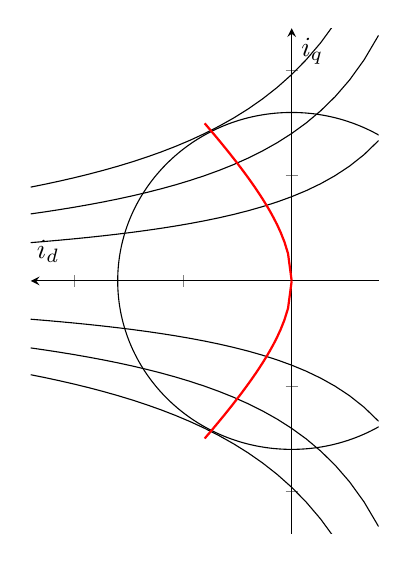
\begin{tikzpicture}
    \begin{axis}[
        axis lines=middle,
        width=6cm,
        height=8cm,
        xlabel={$i_d$},
        x label style={at={(axis description cs:0.05,0.6)},anchor=north},
        ylabel={$i_q$},
        %y label style={at={(axis description cs:0.95,0.05}},
        grid=none,
        xmin=-1.2,
        xmax=0.4,
        ymin=-1.2,
        ymax=1.2,
        no markers,
        x axis line style = {stealth-},
        xticklabels=\empty,  % Elimina las marcas en el eje x
        yticklabels=\empty,  % Elimina las marcas en el eje y
    ]
    
    \draw[black] (0,0) circle [radius=0.8];
    \addplot[black, domain=-1.2:0.4] {4*0.4/(3*2*((2/3)+(2/3)/1*(1-2)*x))};
    \addplot[black, domain=-1.2:0.4] {4*0.7/(3*2*((2/3)+(2/3)/1*(1-2)*x))};
    \addplot[black, domain=-1.2:0.4] {4*0.98/(3*2*((2/3)+(2/3)/1*(1-2)*x))};
    
    \addplot[black, domain=-1.2:0.4] {-4*0.4/(3*2*((2/3)+(2/3)/1*(1-2)*x))};
    \addplot[black, domain=-1.2:0.4] {-4*0.7/(3*2*((2/3)+(2/3)/1*(1-2)*x))};
    \addplot[black, domain=-1.2:0.4] {-4*0.98/(3*2*((2/3)+(2/3)/1*(1-2)*x))};
    
    \addplot[red, thick, domain=-0.4:0] {sqrt(((2/3)*x+(2/3)*(1-2)*x^2)/((2/3)*(1-2))))};
    \addplot[red, thick, domain=-0.4:0] {-sqrt(((2/3)*x+(2/3)*(1-2)*x^2)/((2/3)*(1-2))))};


    \end{axis}
    \end{tikzpicture}
  \caption{Trayectoria MTPA.}
\end{figure}


\subsubsection{CTC (Curva de Torque Constante)}

Como se puede observar, las hipérbolas de torque definen una trayectoria la cual permite mantener un par constante. Recordando las elipses de tensión, para un mismo valor de $V_s$ las elipses se contraen hacia el foco a medida que la velocidad aumenta. Esto significa que siguiendo la curva de torque constante de derecha a izquierda se puede mantener el par aumentando la velocidad. Usando la expresión \ref{eq_tq_pol} se puede obtener directamente:
\begin{equation*}
	T_{em} = \frac{3}{2}pp\cdot((L_d - L_q)\cdot I_s^2 \cdot \sin(\gamma)\cos(\gamma) + \lambda_m\cdot I_s\cdot \sin(\gamma))
\end{equation*}

\begin{equation}
I_{s,\text{CTC}} = \frac{\lambda_m}{L_d} \cdot \frac{\sqrt{\sin(\gamma)^2+\frac{2\cdot\frac{L_d-L_q}{L_d}\cdot\sin(2\gamma)\cdot T_{em}\cdot2 L_d}{3\cdot pp \cdot \lambda_m^2}}-\sin(\gamma)}{\sin(2\gamma)\cdot(\frac{L_d-L_q}{L_d})}
\end{equation}



\begin{figure}[H]
  \centering
    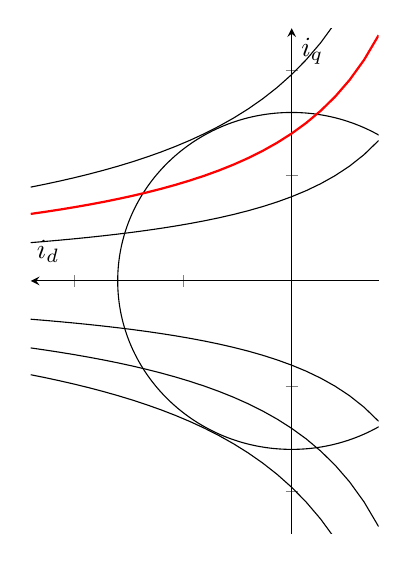
\begin{tikzpicture}
    \begin{axis}[
        axis lines=middle,
        width=6cm,
        height=8cm,
        xlabel={$i_d$},
        x label style={at={(axis description cs:0.05,0.6)},anchor=north},
        ylabel={$i_q$},
        %y label style={at={(axis description cs:0.95,0.05}},
        grid=none,
        xmin=-1.2,
        xmax=0.4,
        ymin=-1.2,
        ymax=1.2,
        no markers,
        x axis line style = {stealth-},
        xticklabels=\empty,  % Elimina las marcas en el eje x
        yticklabels=\empty,  % Elimina las marcas en el eje y
    ]
    
    \draw[black] (0,0) circle [radius=0.8];
    \addplot[black, domain=-1.2:0.4] {4*0.4/(3*2*((2/3)+(2/3)/1*(1-2)*x))};
    \addplot[red, thick, domain=-1.2:0.4] {4*0.7/(3*2*((2/3)+(2/3)/1*(1-2)*x))};
    \addplot[black, domain=-1.2:0.4] {4*0.98/(3*2*((2/3)+(2/3)/1*(1-2)*x))};
    
    \addplot[black, domain=-1.2:0.4] {-4*0.4/(3*2*((2/3)+(2/3)/1*(1-2)*x))};
    \addplot[black, domain=-1.2:0.4] {-4*0.7/(3*2*((2/3)+(2/3)/1*(1-2)*x))};
    \addplot[black, domain=-1.2:0.4] {-4*0.98/(3*2*((2/3)+(2/3)/1*(1-2)*x))};
    
    \end{axis}
    \end{tikzpicture}
  \caption{Trayectoria CTC.}
\end{figure}


\subsubsection{MTPV (Máximo Par por Voltio)}

Existe una trayectoria que permite maximizar el par entregado por el motor en rangos de velocidad muy altos donde el límite es la tensión que puede sintetizar la controladora. La condición que se debe cumplir es:

\begin{equation}
\frac{\partial T_{em}}{\partial \delta} = 0
\end{equation}

Donde $\delta$ es el ángulo del vector de tensión $V_s$, de la misma manera que $\gamma$ es el ángulo del vector de corriente $I_s$. La expresión analítica se desarrolla a partir de la expresión de par en coordenadas cartesianas (\ref{eq_tq_dq}):

\begin{equation*}
T_{em} = \frac{3}{2}pp\cdot((L_d - L_q) i_q i_d + \lambda_m i_q)
\end{equation*}

Se aíslan $i_d$ e $i_q$ de \ref{eq_vd} y \ref{eq_vq}, negligiendo la caída de tensión resistiva del estator: 
\begin{equation}
i_d = \frac{v_q}{\omega_e \cdot L_d} - \frac{\lambda_m}{L_d}; i_q = -\frac{v_d}{\omega_e \cdot L_q}
\end{equation}

\begin{equation}
T_{em} = \frac{3}{2}pp\cdot\left((L_d - L_q) (-\frac{v_d}{\omega_e \cdot L_q}) (\frac{v_q}{\omega_e \cdot L_d} - \frac{\lambda_m}{L_d}) + \lambda_m (-\frac{v_d}{\omega_e \cdot L_q})\right)
\end{equation}

\begin{equation}
T_{em} = \frac{3}{2}pp\cdot\left((L_d - L_q) (-\frac{V_s \cdot \cos(\delta)}{\omega_e \cdot L_q}) (\frac{V_s \cdot \sin(\delta)}{\omega_e \cdot L_d} - \frac{\lambda_m}{L_d}) + \lambda_m (-\frac{V_s \cdot \cos(\delta)}{\omega_e \cdot L_q})\right)
\end{equation}

\begin{equation}
\begin{split}
\frac{\partial T_{em}}{\partial \delta} = \frac{3}{2}pp\cdot (
(L_d - L_q) \cdot (\frac{V_s \cdot \sin(\delta)}{\omega_e \cdot L_q}) \cdot (\frac{V_s \cdot \sin(\delta)}{\omega_e \cdot L_d} - \frac{\lambda_m}{L_d})\\
-\left(\frac{V_s \cdot \cos(\delta)}{\omega_e}\right)^2 \cdot \frac{L_d - L_q}{L_d\cdot L_q}\\ 
-\frac{\lambda_m \cdot V_s \cdot \sin(\delta)}{L_q \cdot \omega_e} ) = 0
\end{split}
\end{equation}


\begin{equation}
\begin{split}
I_{s,MTPV} = \frac{\lambda_m}{L_d} ( \frac{-(2 - \frac{L_q}{L_d}) \cos(\gamma)}{2(1 - \frac{L_q}{L_d})(1 + (\frac{L_q}{L_d})^2) \cos(\gamma)^2 - 2(1 - \frac{L_q}{L_d}) (\frac{L_q}{L_d})^2}\\
-\frac{\sqrt{(2 - \frac{L_q}{L_d})^2 \cos(\gamma)^2 - 4(1 - \frac{L_q}{L_d})(1 + (\frac{L_q}{L_d})^2) \cos(\gamma)^2 - 4(1 - \frac{L_q}{L_d}) (\frac{L_q}{L_d})^2}}{2(1 - \frac{L_q}{L_d})(1 + (\frac{L_q}{L_d})^2) \cos(\gamma)^2 - 2(1 - \frac{L_q}{L_d}) (\frac{L_q}{L_d})^2} )
\end{split}
\end{equation}




Cabe destacar que esta trayectoria solamente se puede ejecutar si se cumple la condición de que $I_{sc} \leq I_{s,max}$.


\begin{figure}[H]
  \centering
    \begin{tikzpicture}
    \begin{axis}[
        axis lines=middle,
        width=6cm,
        height=8cm,
        xlabel={$i_d$},
        x label style={at={(axis description cs:0.05,0.6)},anchor=north},
        ylabel={$i_q$},
        %y label style={at={(axis description cs:0.95,0.05}},
        grid=none,
        xmin=-1.2,
        xmax=0.4,
        ymin=-1.2,
        ymax=1.2,
        no markers,
        x axis line style = {stealth-},
        xtick = {-0.6},
        xticklabels={$-\frac{\lambda_m}{L_d}$},  % Elimina las marcas en el eje x
        yticklabels=\empty,  % Elimina las marcas en el eje y
    ]
    
    
    \draw[black] (0,0) circle [radius=0.8];
    \addplot[red, thick, domain=-0.77:-0.6] {0.5*sqrt(4*(1.111111)^2*(x^2-x*0)+(1.111111)^2*0^2-2.22222222^2*0.6^2)/2.22222222};


    \end{axis}
    \end{tikzpicture}
  \caption{Trayectoria MTPV.}
\end{figure}



\subsubsection{CVL (Límites de Corriente y Voltaje)}

Por último, se presentan los límites eléctricos del motor y del convertidor. El límite de corriente consiste simplemente en saturar la magnitud de la corriente de manera que no sobrepase el valor máximo establecido. La trayectoria sería sencillamente seguir el círculo de corriente anteriormente presentado (CLC), con la siguiente expresión:

\[
I_{s,\text{CLC}} = I_{s,\text{max}} , \forall \gamma \in [0,2\pi]
\]


\begin{figure}[H]
  \centering
    \begin{tikzpicture}
    \begin{axis}[
        axis lines=middle,
        width=6cm,
        height=8cm,
        xlabel={$i_d$},
        x label style={at={(axis description cs:0.05,0.6)},anchor=north},
        ylabel={$i_q$},
        %y label style={at={(axis description cs:0.95,0.05}},
        grid=none,
        xmin=-1.2,
        xmax=0.4,
        ymin=-1.2,
        ymax=1.2,
        no markers,
        x axis line style = {stealth-},
        xticklabels=\empty,  % Elimina las marcas en el eje x
        yticklabels=\empty,  % Elimina las marcas en el eje y
    ]
    
    % Límite de corriente Is_max
    \draw[red, thick] (0,0) circle [radius=0.8];

    \end{axis}
    \end{tikzpicture}
  \caption{Trayectoria CLC.}
\end{figure}


El límite de tensión del motor en realidad se puede entender como la velocidad máxima a la que se puede llegar con una determinada tensión. Por ello, se usa la expresión de las elipses de tensión (VLE):

\begin{equation}
1 \geq \frac{\left(\frac{\lambda_m}{L_d}+I_s \cdot \cos(\gamma)\right)^2}{\left(\frac{\frac{V_{DC}}{\sqrt{3}}}{L_d\cdot\omega_e}\right)^2}+\frac{(I_s \cdot \sin(\gamma))^2}{\left(\frac{\frac{V_{DC}}{\sqrt{3}}}{L_q\cdot\omega_e}\right)^2}
\end{equation}

Igual que para el resto de trayectorias, se debe obtener una expresión de la elipse en función de $I_s$ y $\gamma$. Ya que no es trivial despejar estas variables de la expresión anterior, se manipula usando la ecuación polar de la elipse desplazada del origen:
\begin{equation}
\rho(\theta) = \frac{b^2 x \cos (\theta ) + a^2 y \sin (\theta )\pm a b \sqrt{\left(a^2-x^2\right) \sin ^2(\theta )+\left(b^2-y^2\right) \cos ^2(\theta )+2 x y \sin (\theta ) \cos (\theta )}}{a^2 \sin ^2(\theta )+b^2 \cos ^2(\theta )}
\end{equation}

Dado que estas elipses tan solo están desplazadas en el eje $x$, se pueden eliminar todos los términos referentes al desplazamiento en $y$.
\begin{equation}
\rho(\theta) = \frac{b^2 x \cos (\theta ) \pm a b \sqrt{\left(a^2-x^2\right) \sin ^2(\theta )+\left(b^2\right) \cos ^2(\theta )}}{a^2 \sin ^2(\theta )+b^2 \cos ^2(\theta )}
\end{equation}

Sustituyendo por los términos conocidos y simplificando:

\begin{equation}
	=\frac{\left(\frac{1}{L_q}\right)^2\left(-I_{s c}\right) \cos (\gamma) \pm \frac{1}{L_d \cdot L_q} \sqrt{\left(\left(\frac{V_s}{L_d \cdot \omega_e}\right)^2-\left(-I_{s c}\right)^2\right) \sin ^2(\gamma)+\left(\frac{V_s}{L_q \cdot \omega_e}\right)^2 \cos ^2(\gamma)}}{\left(\frac{1}{L_d}\right)^2 \sin ^2(\gamma)+\left(\frac{1}{L_q}\right)^2 \cos ^2(\gamma)}
\end{equation}


\begin{figure}[H]
  \centering
    \begin{tikzpicture}
    \begin{axis}[
        axis lines=middle,
        width=6cm,
        height=8cm,
        xlabel={$i_d$},
        x label style={at={(axis description cs:0.05,0.6)},anchor=north},
        ylabel={$i_q$},
        %y label style={at={(axis description cs:0.95,0.05}},
        grid=none,
        xmin=-1.2,
        xmax=0.4,
        ymin=-1.2,
        ymax=1.2,
        no markers,
        x axis line style = {stealth-},
        xtick = {-1},
        xticklabels={$-\frac{\lambda_m}{L_d}$},  % Elimina las marcas en el eje x
        yticklabels=\empty,  % Elimina las marcas en el eje y
    ]
    
    
    \draw[black] (0,0) circle [radius=0.8];

    \draw[red, thick] (-1,0) ellipse (0.5 and 0.25);


    \end{axis}
    \end{tikzpicture}
  \caption{Trayectoria VLE.}
\end{figure}



Además, el inversor es capaz de sintetizar un máximo de $V_s = \frac{V_{DC}}{\sqrt{3}}$ utilizando SVPWM, por lo tanto, se debe saturar la consigna de tensión a ese valor. Adicionalmente, por seguridad, se multiplica por un factor de seguridad $K_{FW} \in (0,1)$.

\begin{equation}
	V_{s,\text{max}} \leq \frac{V_{DC}}{\sqrt{3}}\cdot K_{FW}
\end{equation}

\subsection{Diseño y simulación del control}

En esta sección, se aborda la implementación del modelo matemático del PMSM en un entorno de simulación. Además, se detallan los pasos cruciales en el diseño del control, destacando la implementación del lazo de control de corriente, el modelo promediado y conmutado del inversor, o la integración de las trayectorias y la estrategia de debilitamiento de campo. Disponer de un modelo de simulación completo permite ganar mucha comprensión sobre el sistema estudiado, pero por el coste computacional suele ser inviable juntar muchos sistemas en una misma simulación.

\subsubsection{EMR (Representación macroscópica energética)}
En primer lugar, se tratará de crear un modelo que permita simular la dinámica electromecánica del PMSM, así como el entorno mecánico en el que se encuentra (vehículo eléctrico) e integrar el control vectorial. Para ello se usará un estándar para modelizar sistemas de potencia, la representación macroscópica energética o EMR por sus siglas en inglés. El concepto se basa en agrupar o dividir las diferentes etapas en las que la potencia se transforma, utilizando el principio de acción-reacción y el principio causal (el efecto causa-efecto causa efecto porque la causa del efecto causa-efecto es a su vez causa y efecto). 

En primer lugar se modeliza la planta eléctrica del PMSM. Se utiliza el modelo con el marco de referencia rotativo $d-q$ por su sencillez. Para ello se implementan las diferentes ecuaciones del motor en bloques separados siguiendo el estándar de la EMR.

\begin{figure}[H]
    \centering
    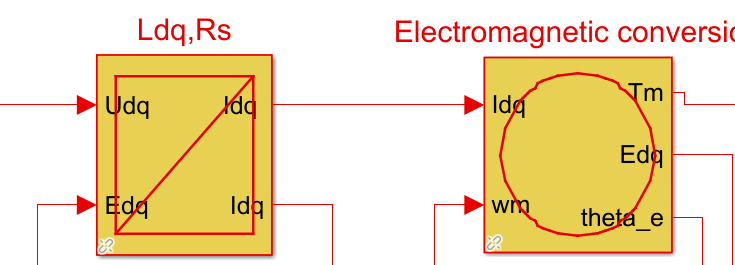
\includegraphics[width=0.7\linewidth]{fig/motorEMR1.png}
    \caption{Bloques que representan el PMSM.}
\end{figure}

\begin{figure}[H]
    \centering
    \begin{subfigure}{0.52\linewidth}
        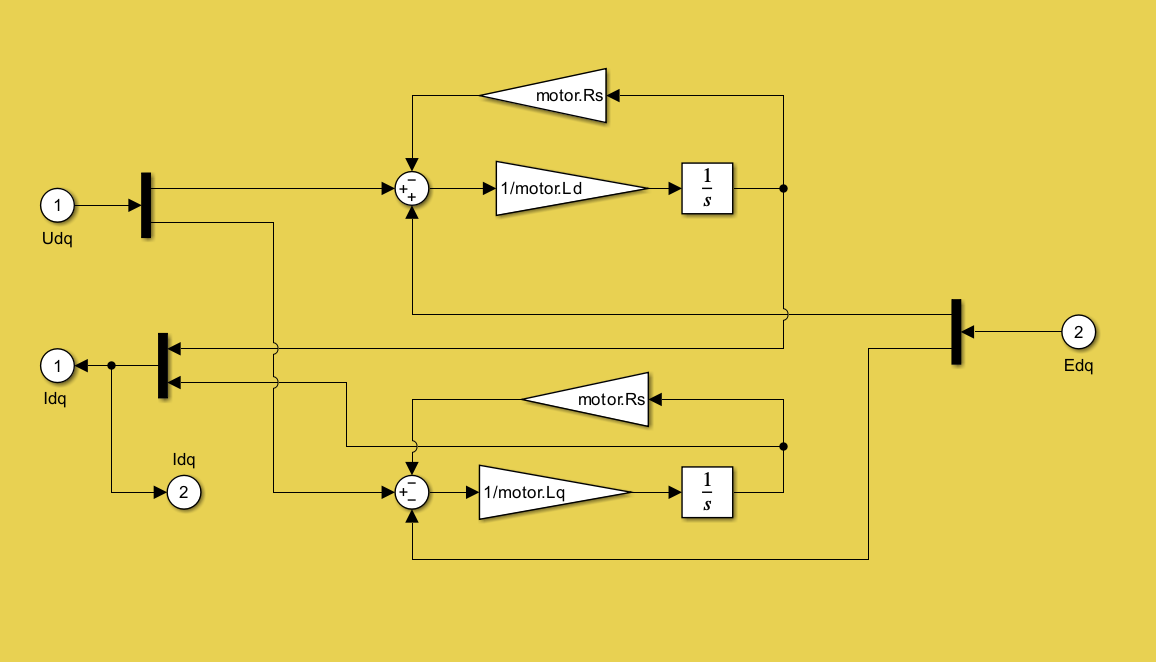
\includegraphics[width=\linewidth]{fig/motorEMR2.png}
        \caption{Circuito eléctrico.}
    \end{subfigure}
    \begin{subfigure}{0.4\linewidth}
        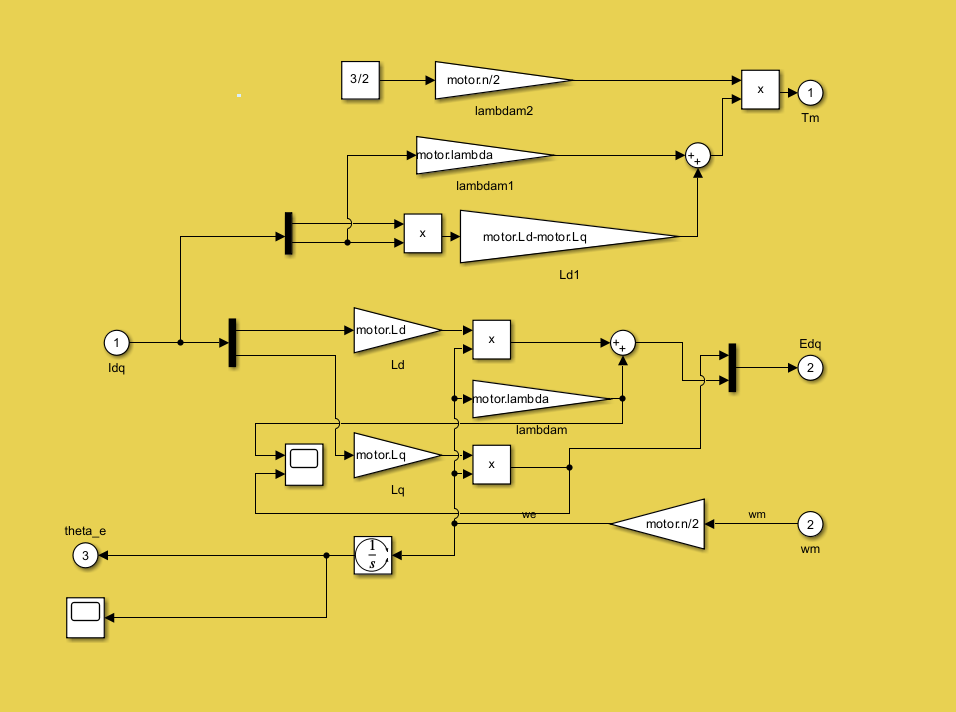
\includegraphics[width=\linewidth]{fig/motorEMR3.png}
        \caption{Conversión electromecánica}
    \end{subfigure}
    \caption{Detalle de los bloques del PMSM}
\end{figure}

También se modela la planta mecánica del motor, así como la transmisión de la potencia mecánica a las ruedas y al vehículo.

\begin{figure}[H]
    \centering
    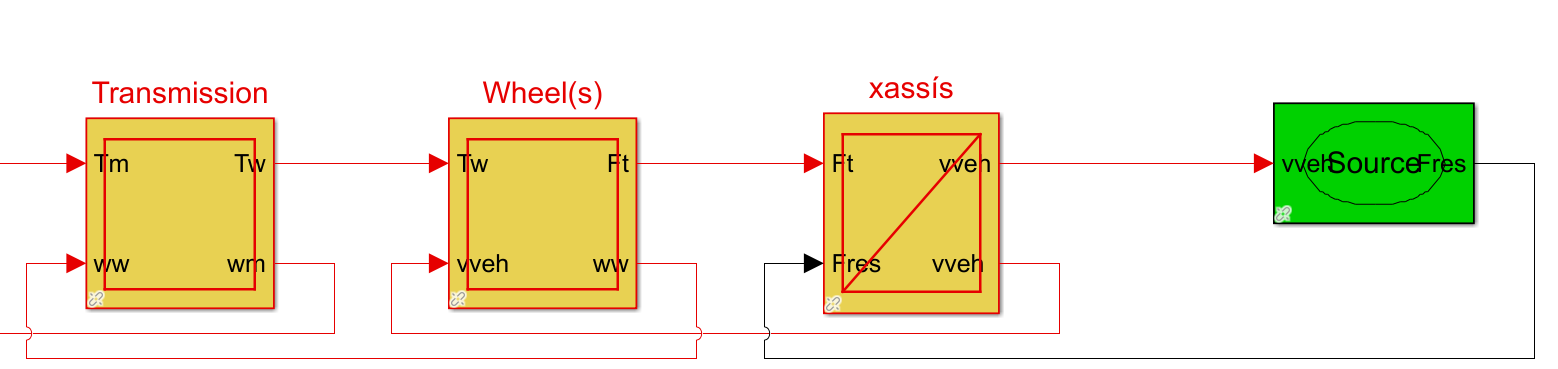
\includegraphics[width=0.95\linewidth]{fig/carEMR.png}
    \caption{Planta mecánica.}
\end{figure}

\subsubsection{Lazos de corriente y modelo promediado del inversor}

Como se ha visto hasta ahora, es práctico utilizar la corriente para controlar el motor. Por ello, se implementa un lazo de corriente utilizando controladores PI para el eje $d$ y para el eje $q$ por separado. Como el inversor se utiliza como fuente de tensión, la salida de estos PI es la consigna de tensión. Dado que el motor genera una fuerza contraelectromotriz, se añade como \textit{feed-forward} a los controladores. La salida del controlador no se satura directamente, sino que se implementa una saturación posterior la cual se realimenta al controlador para usar una técnica de \textit{anti-windup}. Las constantes de los controladores se ajustan de la siguiente manera:

% PI de corriente, respuesta de segundo orden
\[
M_p = 15 \%
\]

\[
 t_s = T_s \cdot 20
\]
Donde $M_p$ es el sobre-impulso deseado en la respuesta a una entrada de escalón, $t_s$ es el tiempo de establecimiento deseado, y $T_s$ es la inversa de la frecuencia de control.

\begin{equation}
	\xi = \sqrt{\frac{\log(M_p)^2}{\pi^2 + \log(M_p)^2}}
\end{equation}

\begin{equation}
\omega_n = \frac{3}{\xi \cdot t_s}
\end{equation}

\begin{equation}
Kp_{id} = 2 \cdot \xi \cdot \omega_n \cdot L_d - R_s
\end{equation}

\begin{equation}
Ki_{id} = \omega_n^2 \cdot L_d
\end{equation}

\begin{equation}
Kp_{iq} = 2 \cdot \xi \cdot \omega_n \cdot L_q - R_s
\end{equation}

\begin{equation}
Ki_{iq} = \omega_n^2 \cdot L_q \quad
\end{equation}

\begin{figure}[H]
    \begin{subfigure}{0.2\linewidth}
        \centering
        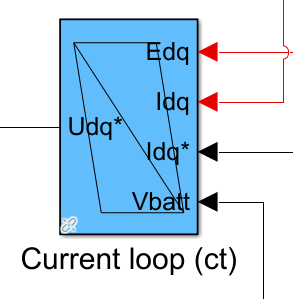
\includegraphics[width=\linewidth]{fig/PIEMR_out.png}
    \end{subfigure}
    \begin{subfigure}{0.75\linewidth}
        \centering
        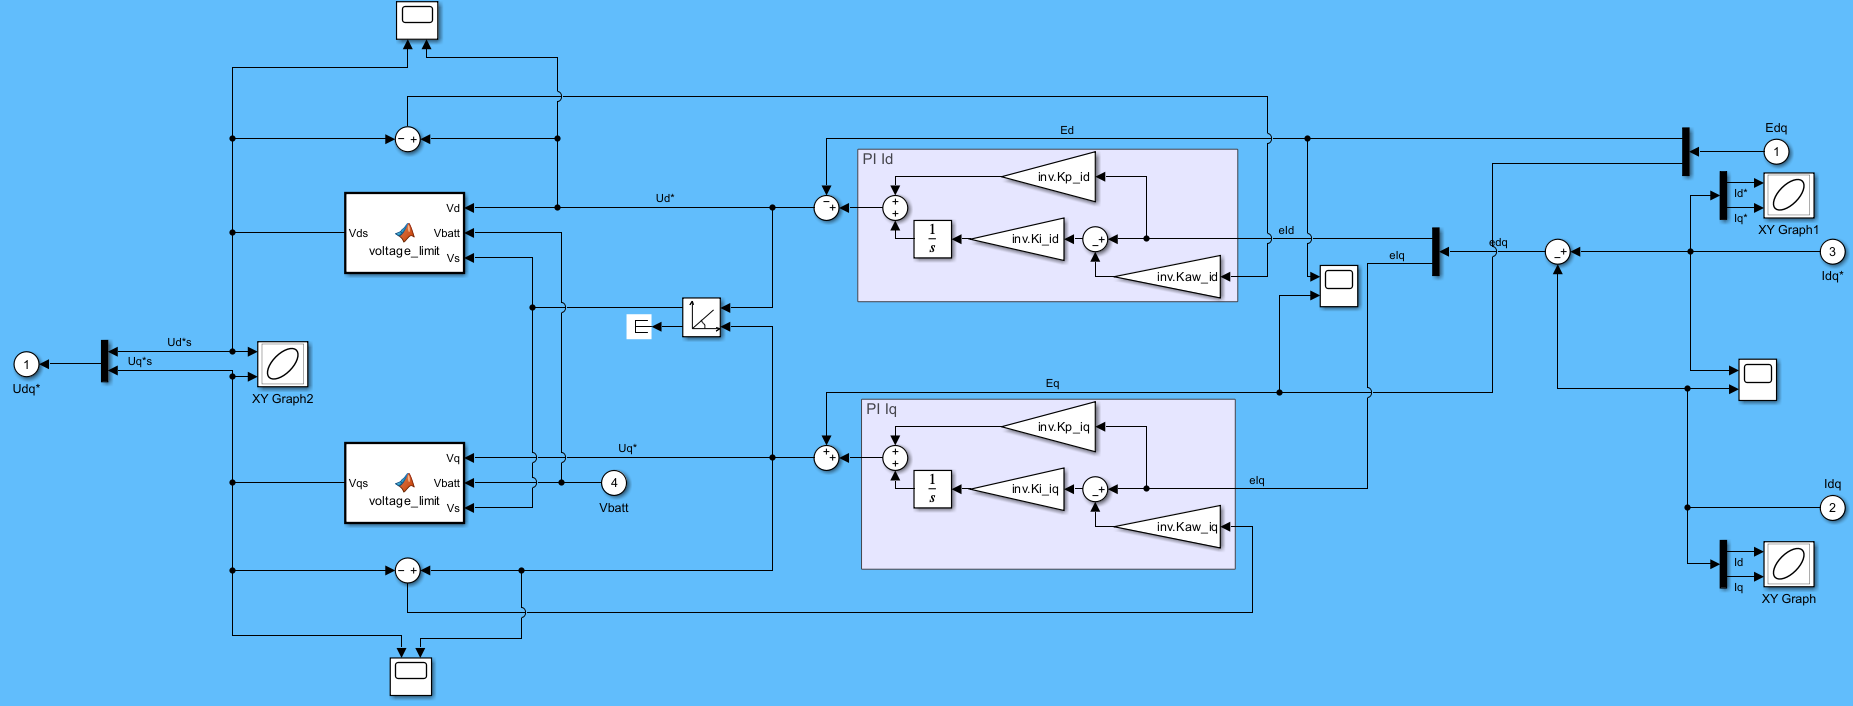
\includegraphics[width=\linewidth]{fig/PIEMR_in.png}
    \end{subfigure}
    \caption{Bloque de los lazos de corriente.}
\end{figure}

Para las simulaciones se han implementado los siguientes parámetros de motor, ya que aunque a fecha de redacción de este documento no está fabricado, se han estimado de manera que se cumplan los requisitos del motor.


\begin{tabular}{|p{2cm}||p{1cm}|p{1.5cm}|p{7cm}|}
 \hline
 \multicolumn{4}{|c|}{Parámetros del Motor} \\
 \hline
 Parámetro & Valor & Unidades & Descripción \\
 \hline
 pp & 3 & ad & Número de pares de polos \\
 $\lambda_m$ & 52.615 & mWb & Flujo magnético de los imanes permanentes \\
 $L_d$ & 188.7 & $\mu$H & Inductancia en el eje d \\
 $L_q$ & 283.1 & $\mu$H & Inductancia en el eje q \\
 $R_s$ & 150 & m$\Omega$ & Resistencia de fase del estator \\
 $\omega_{\text{m,max}}$ & 20000 & rpm & Velocidad angular máxima del motor \\
 $T_{\text{em,max}}$ & 26 & N·m & Par máximo del motor \\
 $V_{\text{bat}}$ & 540 & V & Voltaje de la batería DC \\
 $I_{\text{s,max}}$ & 108 & A & Corriente máxima en los ejes d-q \\
 \hline
\end{tabular}



\begin{figure}[H]
    \centering
    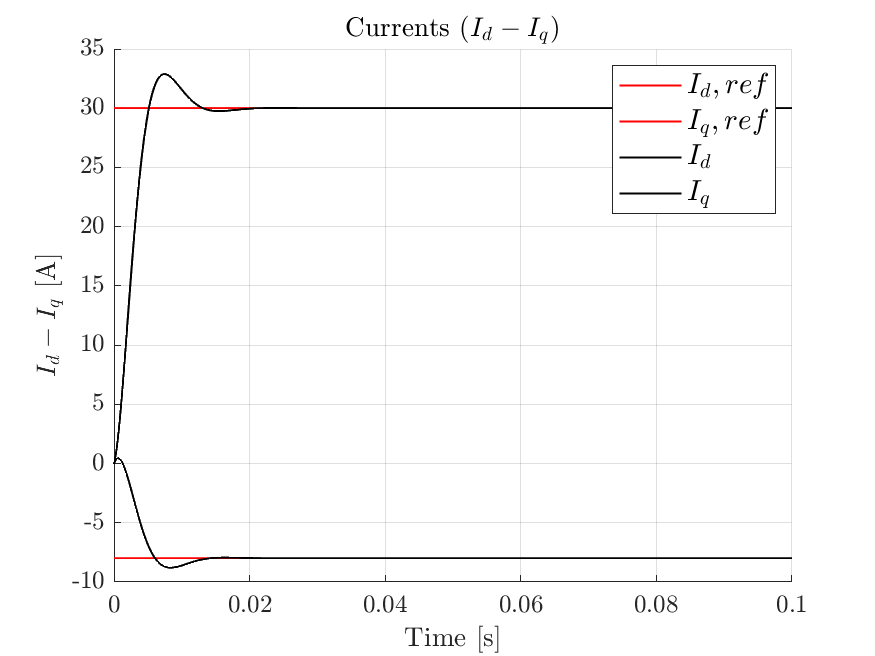
\includegraphics[width=0.75\linewidth]{fig/idiq_plot_PI.png}
    \caption{Simulación de los PIs de corriente, con una consigna de $(i_d, i_q) = (-8, 30) A$.}
\end{figure}


Tras obtener las consignas de tensión, se modela el inversor VSI con SVPWM con un modelo promediado, es decir, sin llegar a generar una señal conmutada por PWM. Se usan relaciones básicas para convertir las magnitudes eléctricas del espacio $d-q$ a DC. Además se incorpora la fuente de energía del sistema, la batería, con un simple modelo RC.

\begin{figure}[H]
    \centering
    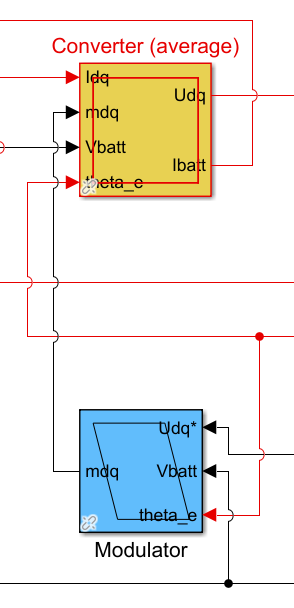
\includegraphics[width=0.25\linewidth]{fig/VSIEMR_out.png}
    \caption{Bloques que contienen el modelo promediado del VSI con SVPWM.}

\end{figure}

\begin{figure}[H]
    \centering
    \begin{subfigure}{0.45\linewidth}
        \centering
        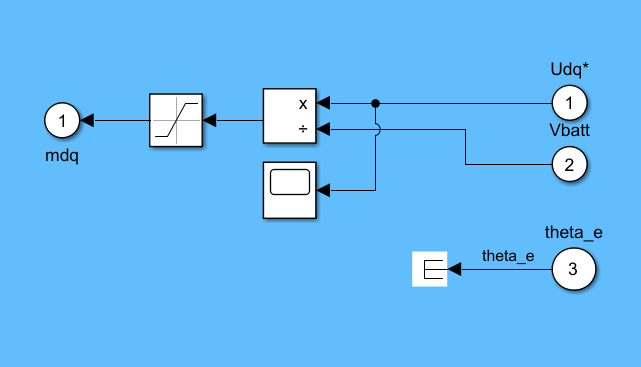
\includegraphics[width=\linewidth]{fig/VSIEMR_in1.png}
    \end{subfigure}
    \begin{subfigure}{0.45\linewidth}
        \centering
        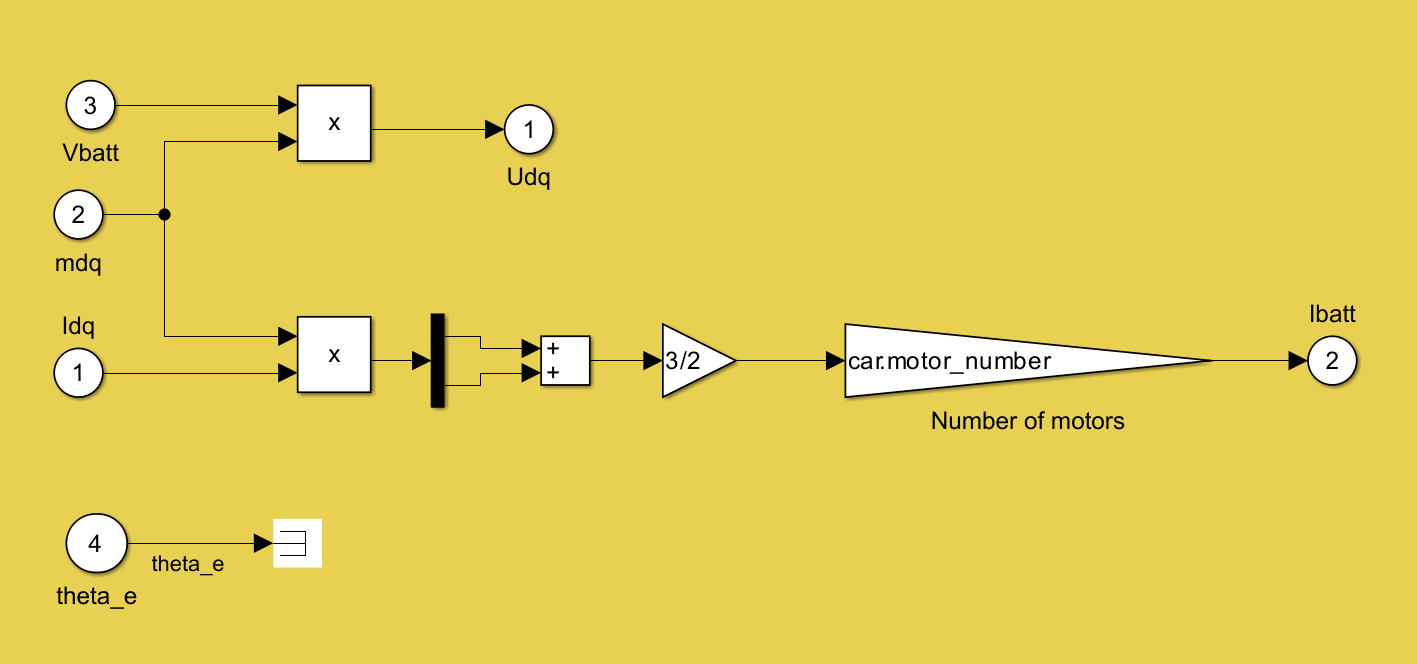
\includegraphics[width=\linewidth]{fig/VSIEMR_in2.png}
    \end{subfigure}
    \caption{Detalle de los bloques del VSI.}

\end{figure}

\subsubsection{Implementación de las trayectorias de control}

Con lo anteriormente desarrollado solamente se pueden consignar las corrientes $i_d$ e $i_q$ manualmente, pero el objetivo es consignar el par y que el propio control sea capaz de gestionar el debilitamiento de campo. Por ello, se implementan las ecuaciones presentadas en el apartado anterior en bloques de código. 

La estrategia es la siguiente: Se implementan las ecuaciones de las trayectorias cuya salida es una corriente (CLC, CTC, MTPV y VLE) y se selecciona la mínima, o en caso de estar en zona de debilitamiento de campo, la óptima, que no necesariamente es la mínima. En paralelo, se calcula el ángulo que correspondería a la trayectoria del MTPA, y se añade un control integral que aumenta el valor del ángulo controlando la tensión para poder entrar en el resto de trayectorias. Este integrador sería justamente el controlador de debilitamiento de campo y se encarga de que la consigna de ángulo no haga sobrepasar el límite de tensión establecido por el bus DC con un cierto factor de seguridad. Se trabaja con módulos de corriente siempre positivos, y ángulos comprendidos entre $\gamma \in [\frac{\pi}{2}, \pi]$. Para obtener par negativo, simplemente se multiplica el ángulo $\gamma$ por el signo de la consigna de par, atendiendo específicamente al caso de par igual a cero.

\begin{figure}[H]
    \centering
    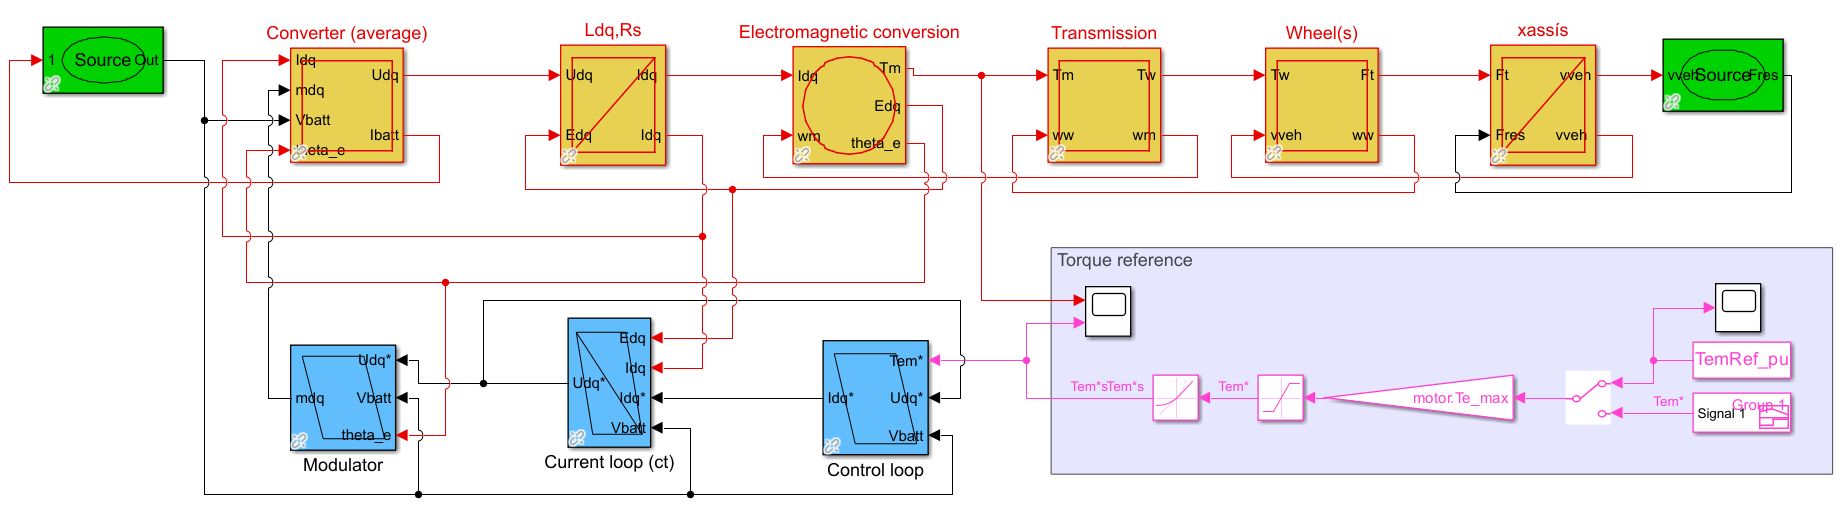
\includegraphics[width=1\linewidth]{fig/EMR_FULL.png}
    \caption{Modelo EMR completo.}
    
\end{figure}

\begin{figure}[H]
    \centering
    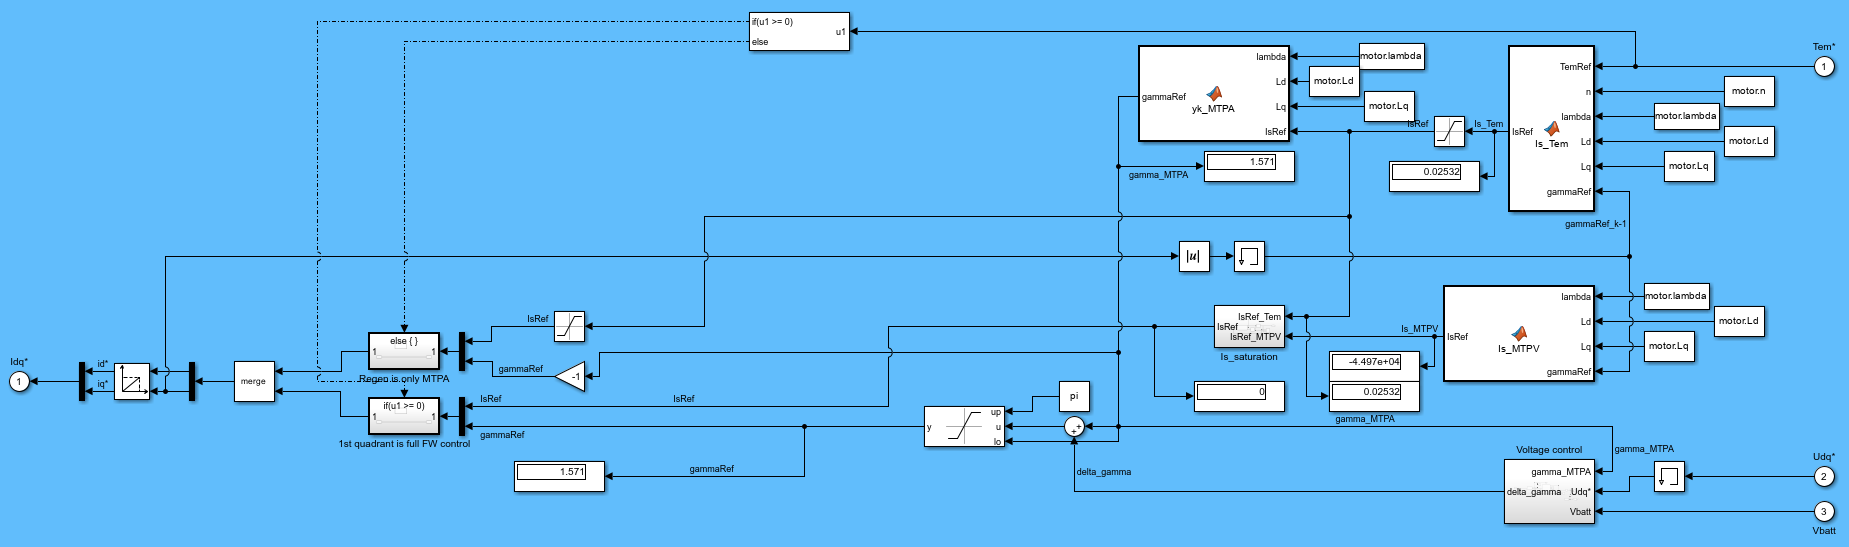
\includegraphics[width=1\linewidth]{fig/EMR_control.png}
    \caption{Detalle del bloque del lazo de control vectorial.}
    
\end{figure}
\newpage
Para comprobar el funcionamiento y la estabilidad del control, se realiza una simulación en la que la consigna de par está extraída de un perfil de conducción real.

\begin{figure}[!htb]
    \centering
    \begin{subfigure}{0.4\textwidth}
        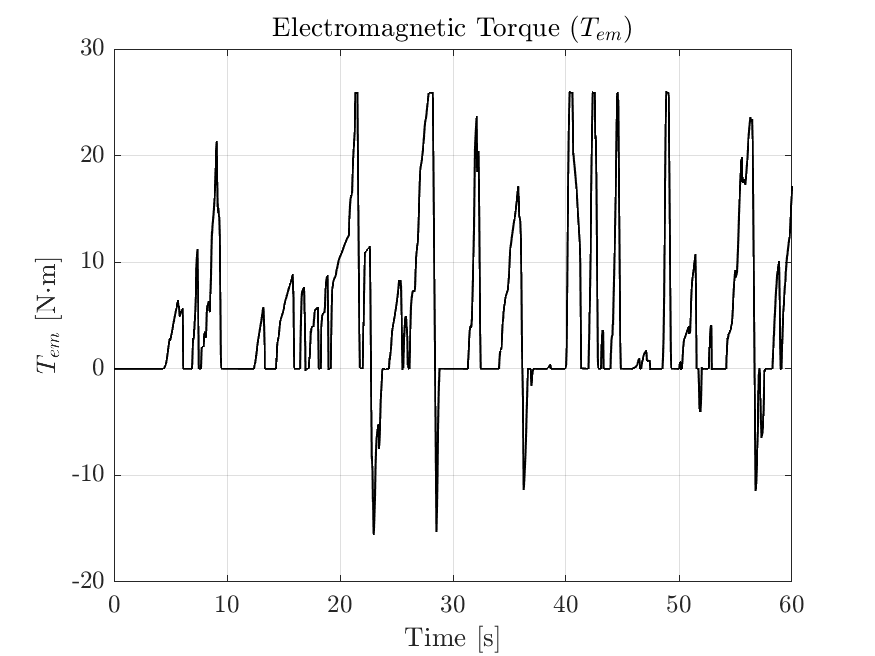
\includegraphics[width=\linewidth]{fig/Tem_plot.png}
        \caption{Torque electromagnético ($T_{em}$).}
    \end{subfigure}
    \begin{subfigure}{0.4\textwidth}
        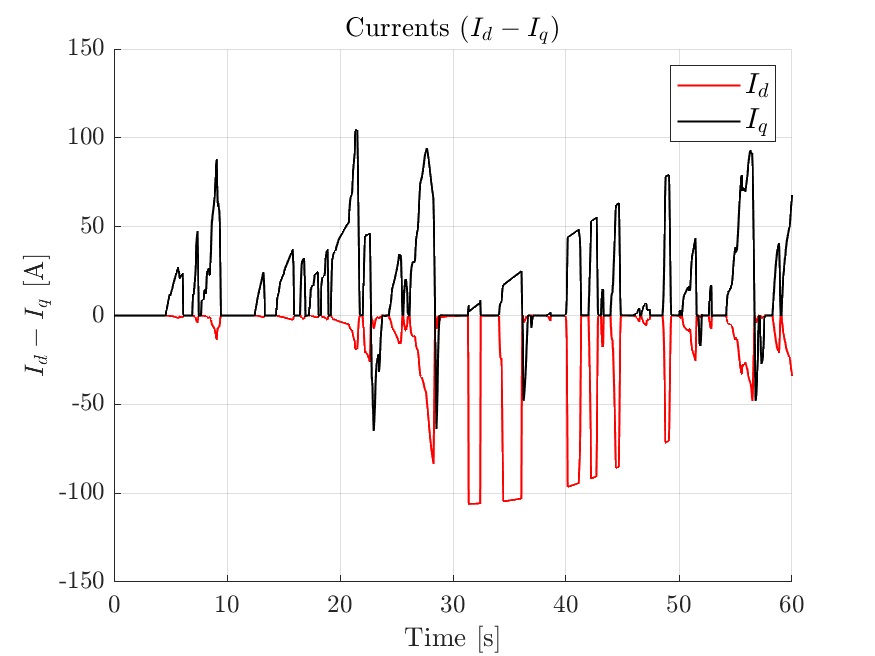
\includegraphics[width=\linewidth]{fig/idiq_plot.png}
        \caption{Corrientes ($I_{d} - I_{q}$).}
    \end{subfigure}
    \begin{subfigure}{0.4\textwidth}
        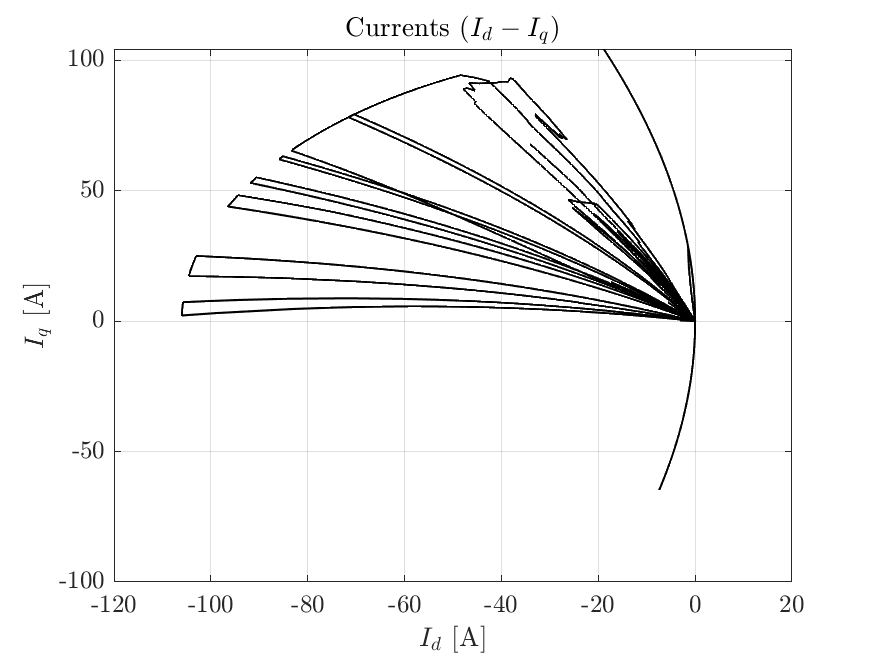
\includegraphics[width=\linewidth]{fig/id-iq_plot.png}
        \caption{Corriente ($I_{d}$) vs Corriente ($I_{q}$).}
    \end{subfigure}
    \begin{subfigure}{0.4\textwidth}
        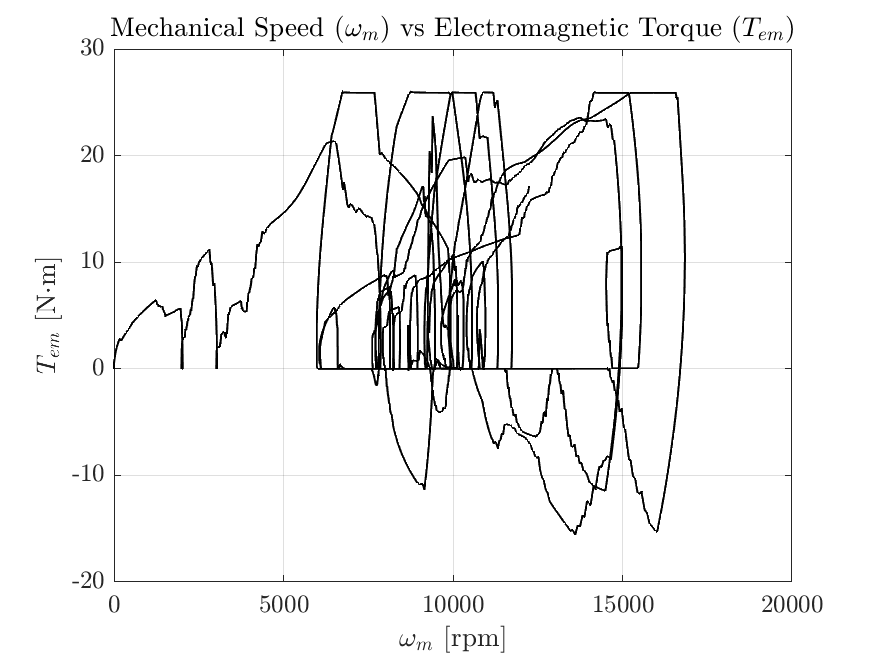
\includegraphics[width=\linewidth]{fig/wm_Tem_plot.png}
        \caption{Velocidad mecánica ($\omega_{m}$) vs Torque electromagnético ($T_{em}$).}
    \end{subfigure}
    \begin{subfigure}{0.4\textwidth}
        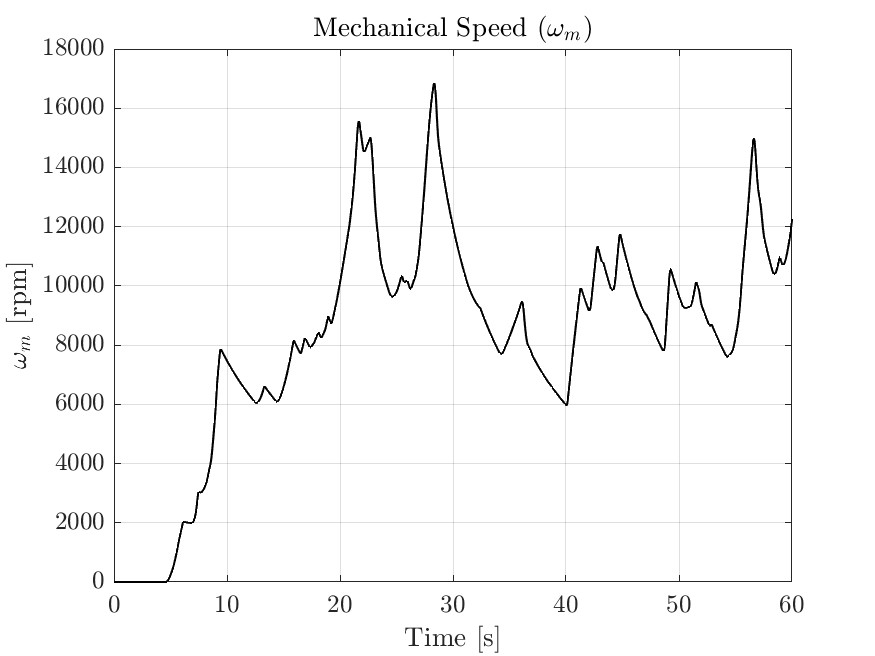
\includegraphics[width=\linewidth]{fig/wm_plot.png}
        \caption{Velocidad mecánica ($\omega_{m}$).}
    \end{subfigure}
    \begin{subfigure}{0.4\textwidth}
        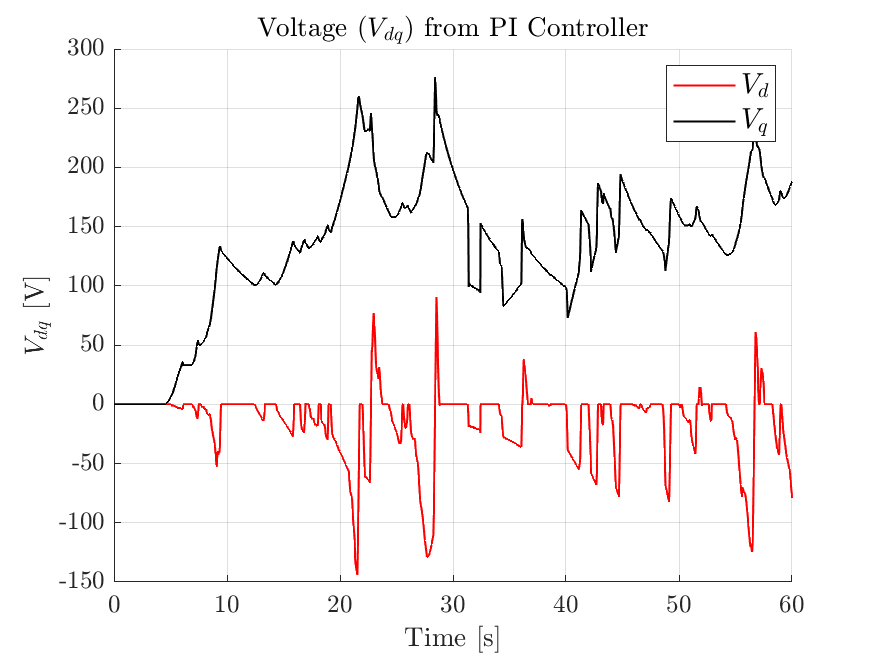
\includegraphics[width=\linewidth]{fig/vdvqPI_plot.png}
        \caption{Voltajes ($V_{d} - V_{q}$).}
    \end{subfigure}
    \caption{Resultados de la simulación.}
    
\end{figure}

Se puede observar que en esta simulación se ha limitado el comportamiento de la frenada regenerativa a la trayectoria del MTPA. Además, se pueden observar ciertos problemas en la implementación del lazo de tensión. Más adelante se realiza una simulación más enfocada en el control que en la aplicación, y en ella se revisan estas situaciones.

\subsubsection{Modelo conmutado}

Dado que el inversor realmente es una fuente conmutada, se debe modelar utilizando una herramienta que lo permita. Utilizando el modelo EMR generado en Simulink se ha implementado la conmutación, pero el tiempo de simulación es demasiado grande como para que sea una herramienta práctica para el desarrollo.

\begin{figure}[H]
    \centering
    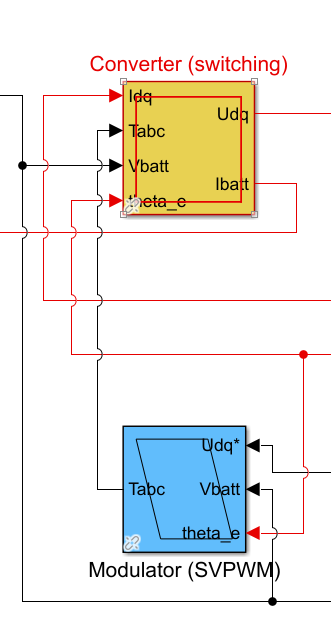
\includegraphics[width=0.25\linewidth]{fig/EMR_VSIsw_out.png}
    \caption{Bloques que contienen el modelo conmutado del VSI con SVPWM.}
    
\end{figure}

\begin{figure}[H]
    \centering

    \begin{subfigure}{0.75\linewidth}
        \centering
        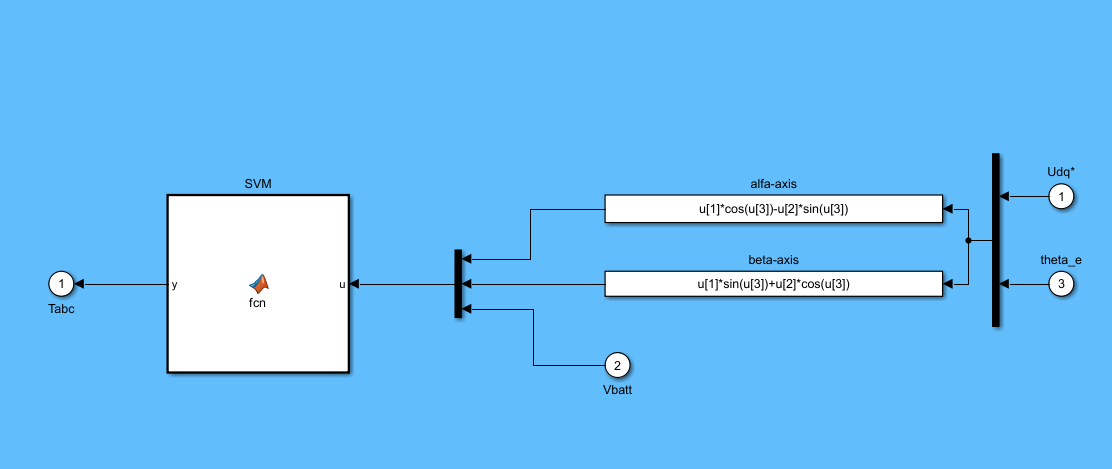
\includegraphics[width=\linewidth]{fig/EMR_VSIsw_in1.png}   
    \end{subfigure}
    \begin{subfigure}{0.75\linewidth}
        \centering
        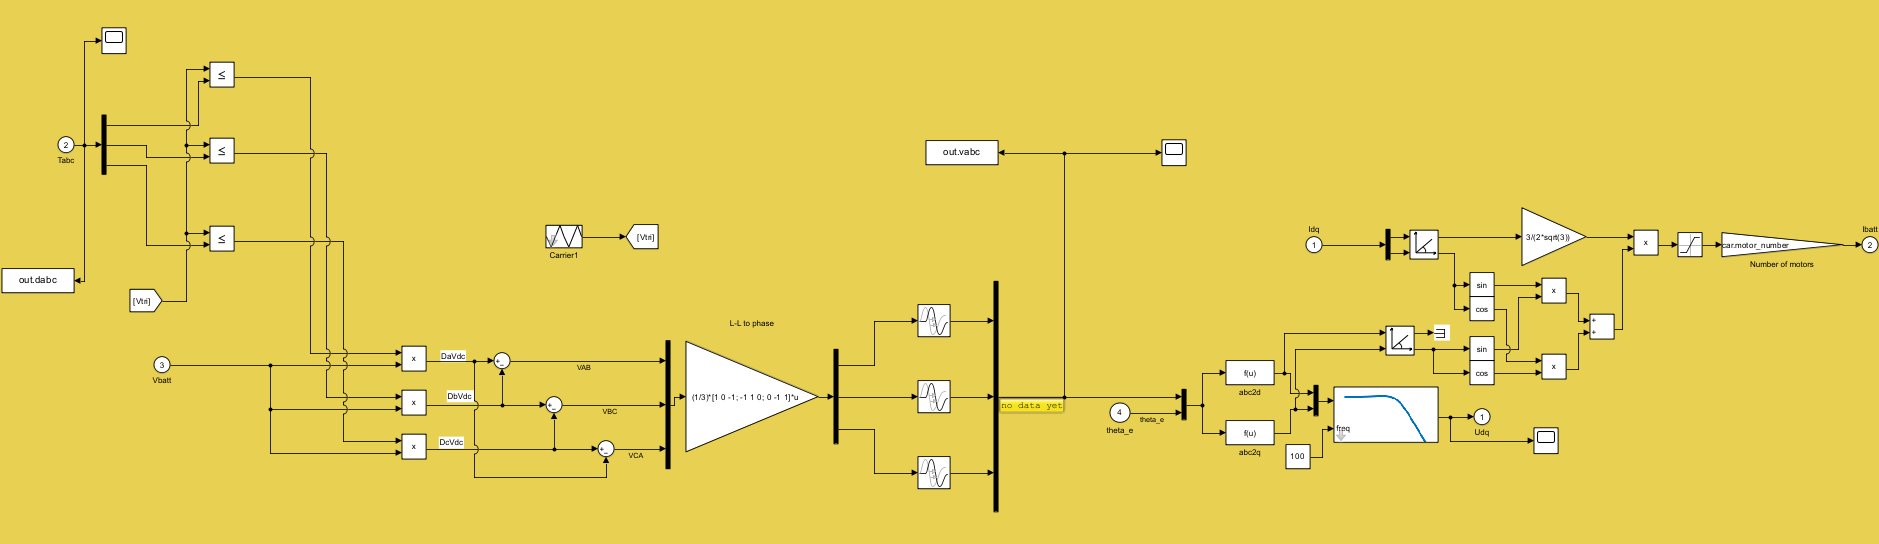
\includegraphics[width=\linewidth]{fig/EMR_VSIsw_in2.png}
    \end{subfigure}
    \caption{Detalle de los bloques del VSI conmutado.}

\end{figure}

\begin{figure}[H]
    \centering
    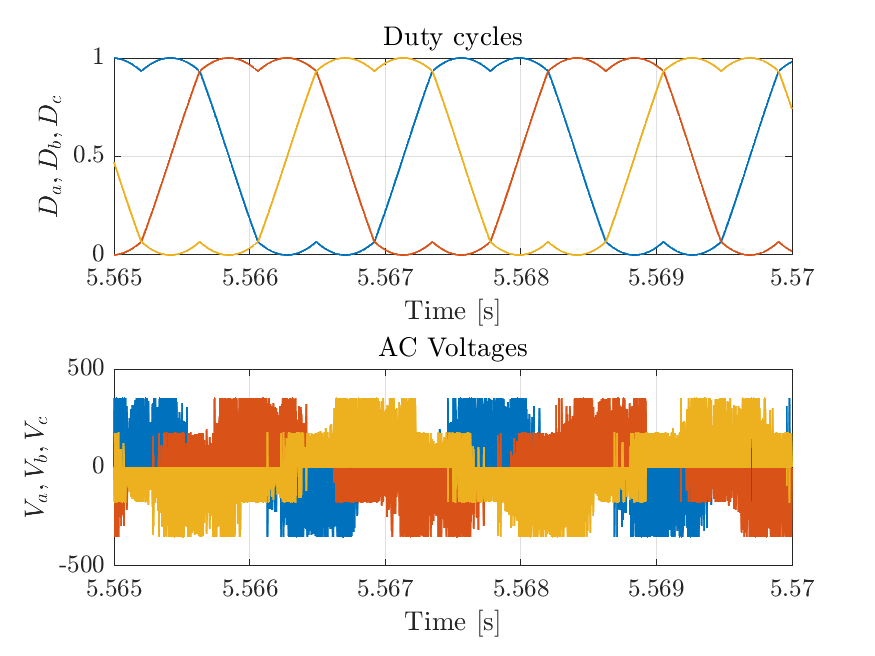
\includegraphics[width=0.85\linewidth]{fig/abc_plot.png}
    \caption{Duty cycles y tensiones alternas.}
    
\end{figure}


Por ello se desarrolla un modelo en PLECS que incorpora el lazo de control, el inversor con MOSFETs, la planta mecánica simplificada, y a la cual se le discretiza la adquisición y el control, de manera que es una aproximación muy realista de la posterior implementación en un microcontrolador. Además se incorporan cálculos térmicos de pérdidas y eficiencia.

\begin{figure}[H]
	\centering
	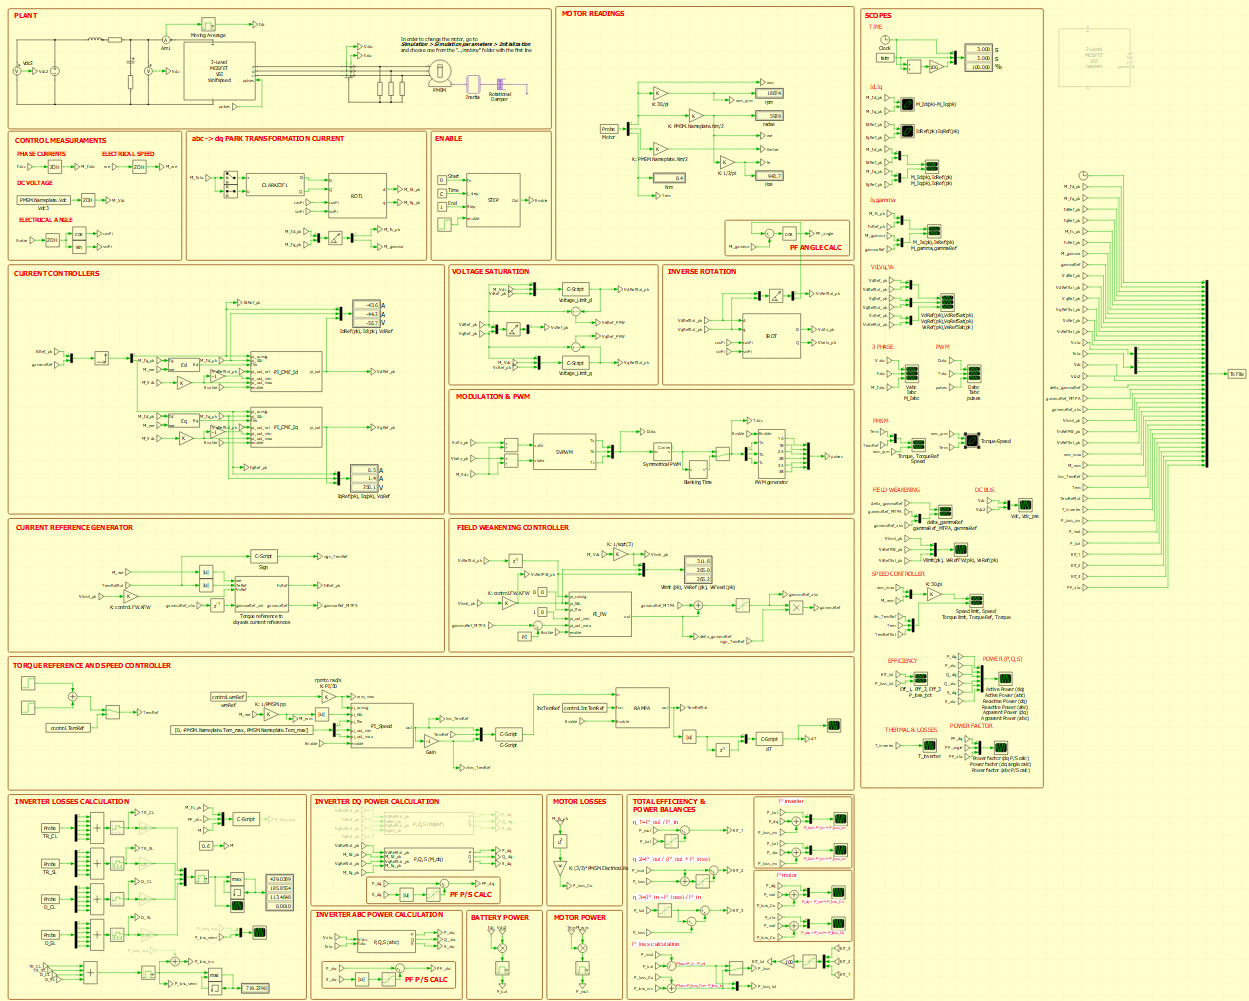
\includegraphics[width=0.7\linewidth]{fig/PLECS_overall}
	\caption{Modelo de simulación en PLECS.}
\end{figure}


Se puede observar que la representación de los bloques en este modelo no sigue el EMR, ya que se elige una implementación más práctica y realista. Destaca la implementación de las funciones de control utilizando la librería PERGAMON, desarrollada por el CITCEA-UPC. Esta librería reproduce completamente el código de las funciones matemáticas implementadas en el control, como los PIs, el SVPWM..., en el software PLECS, lo que facilita la correlación de cualquier modelo con la implementación final en un sistema discreto.


A continuación se presentan los diferentes bloques que forman el modelo.
\begin{figure}[H]
	\centering
	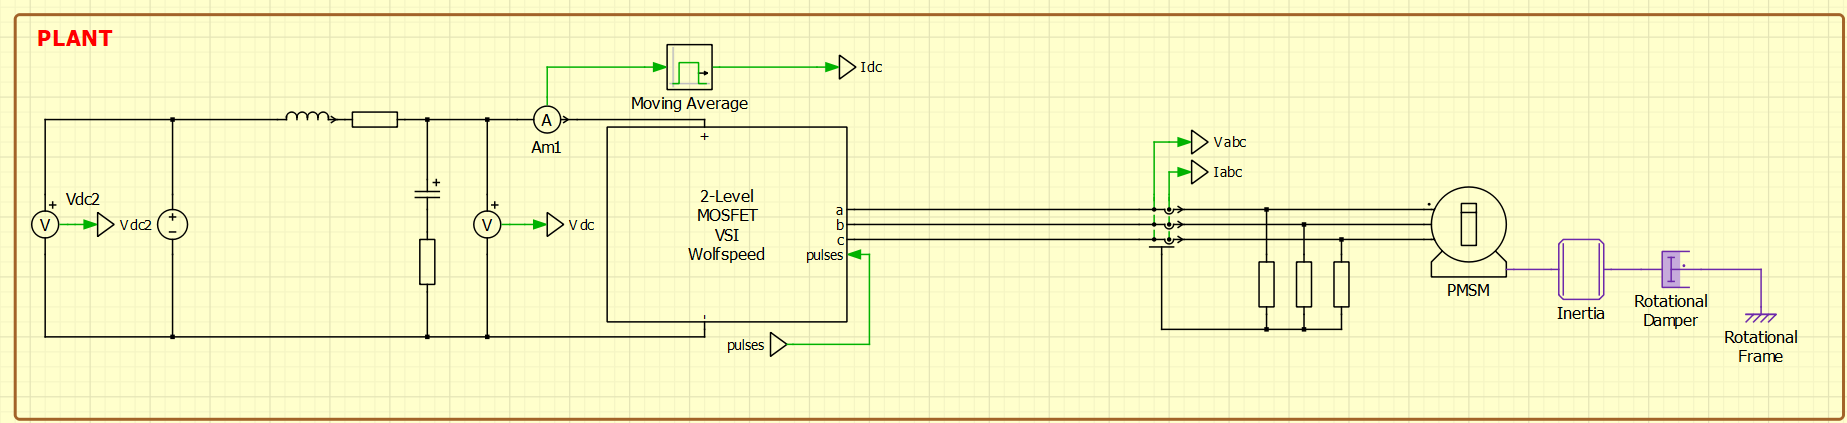
\includegraphics[width=0.7\linewidth]{fig/PLECS_plant}
	\caption{Planta electromecánica del conjunto fuente-inversor-motor-carga.}
\end{figure}

\begin{figure}[H]
	\centering
	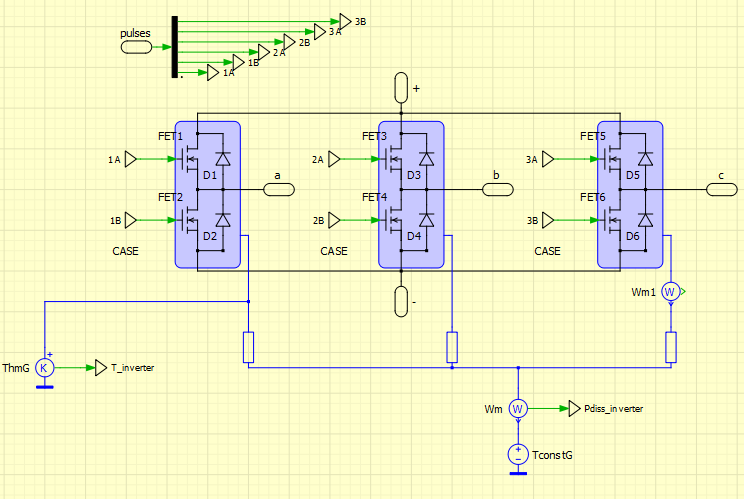
\includegraphics[width=0.7\linewidth]{fig/PLECS_mosfets}
	\caption{Detalle del subbloque VSI, donde se realiza la conexión electrotérmica de los módulos de potencia a la fuente DC, al motor y a la \textit{coldplate}.}
\end{figure}
\begin{figure}[H]
	\centering
	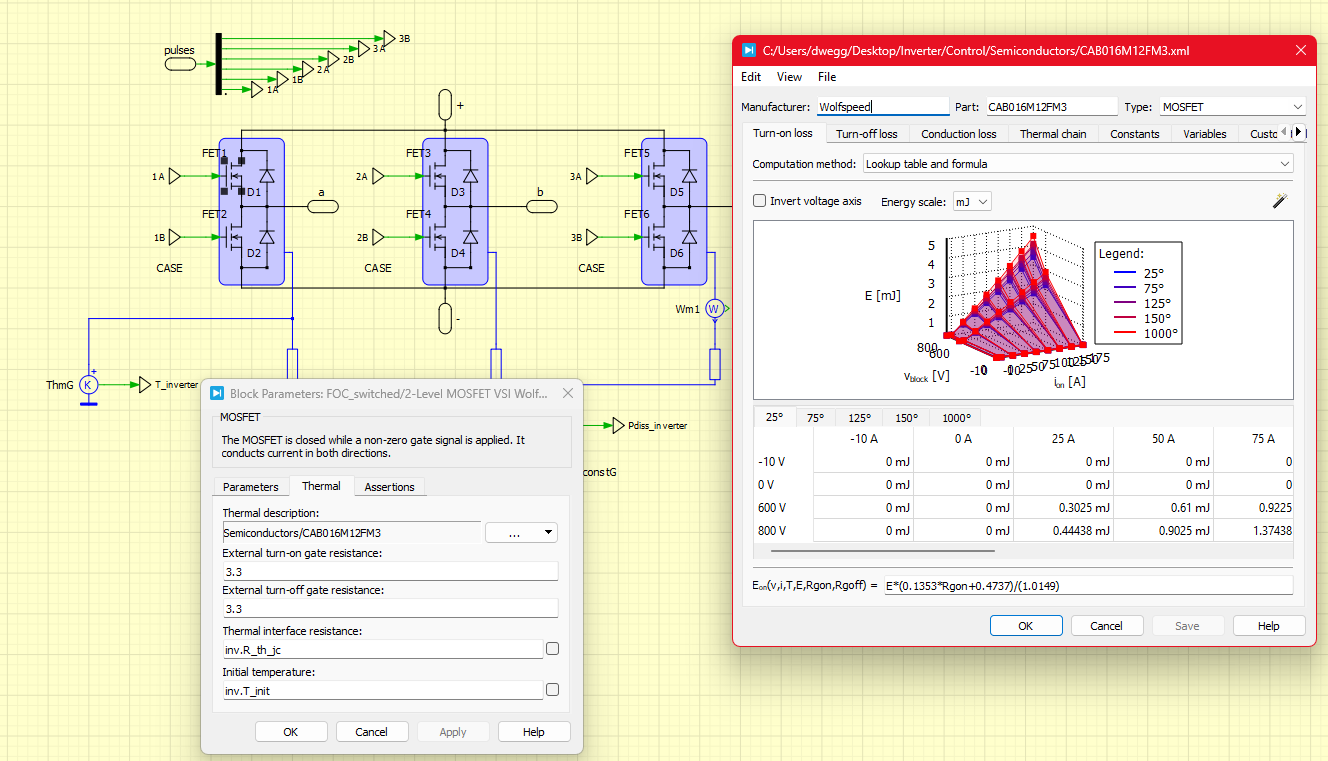
\includegraphics[width=0.7\linewidth]{fig/PLECS_MOSFETs-thermal}
	\caption{Tanto los MOSFETs como los diodos integrados están modelados térmicamente de mano del fabricante, lo que facilita mucho la estimación de pérdidas y la simulación térmica.}
\end{figure}
\begin{figure}[H]
	\centering
	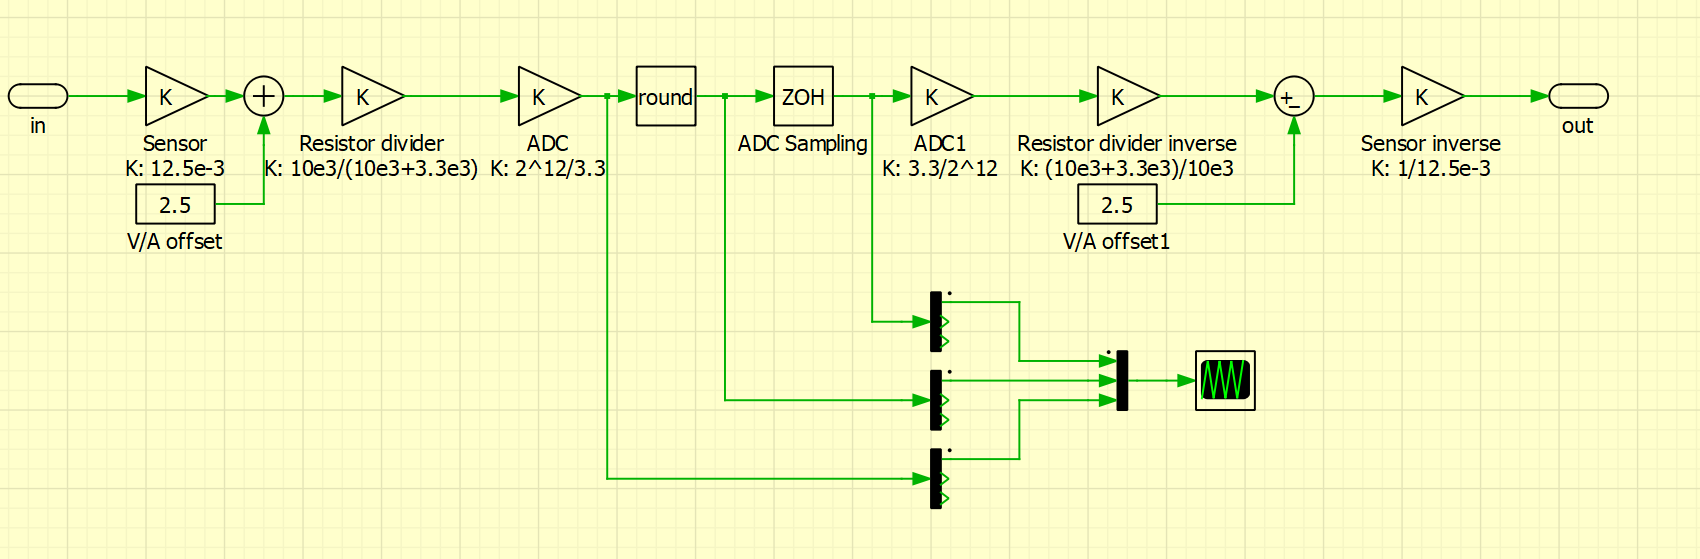
\includegraphics[width=0.7\linewidth]{fig/PLECS_acq}
	\caption{Se modelan los tiempos de adquisición del ADC mediante el uso de \textit{zero order holds}. Se implementa la transformada de las corrientes, tanto de $a,b,c$ al espacio $d-q$ como de coordenadas cartesianas a coordenadas polares.}
\end{figure}
\begin{figure}[H]
	\centering
	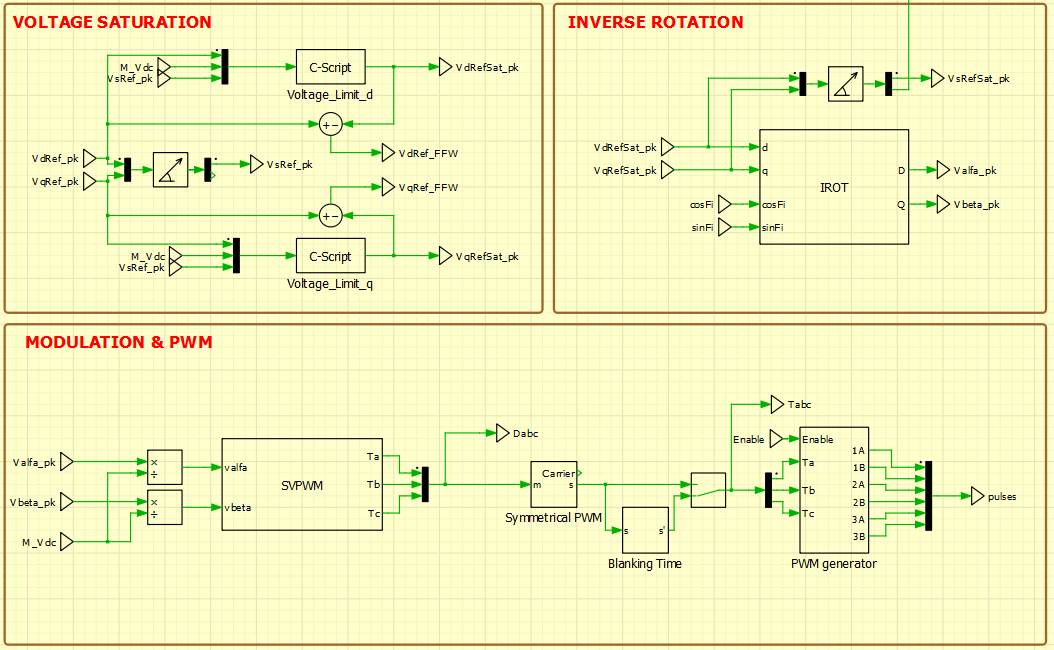
\includegraphics[width=0.7\linewidth]{fig/PLECS_voltage}
	\caption{Saturación y síntesis de las tensiones $V_d$ y $V_q$ mediante la transformada de Clarke inversa y la modulación SVPWM de la librería PERGAMON. Se modelan también los tiempos muertos de la modulación.}
	\label{fig:plecsvoltage}
\end{figure}
\begin{figure}[H]
	\centering
	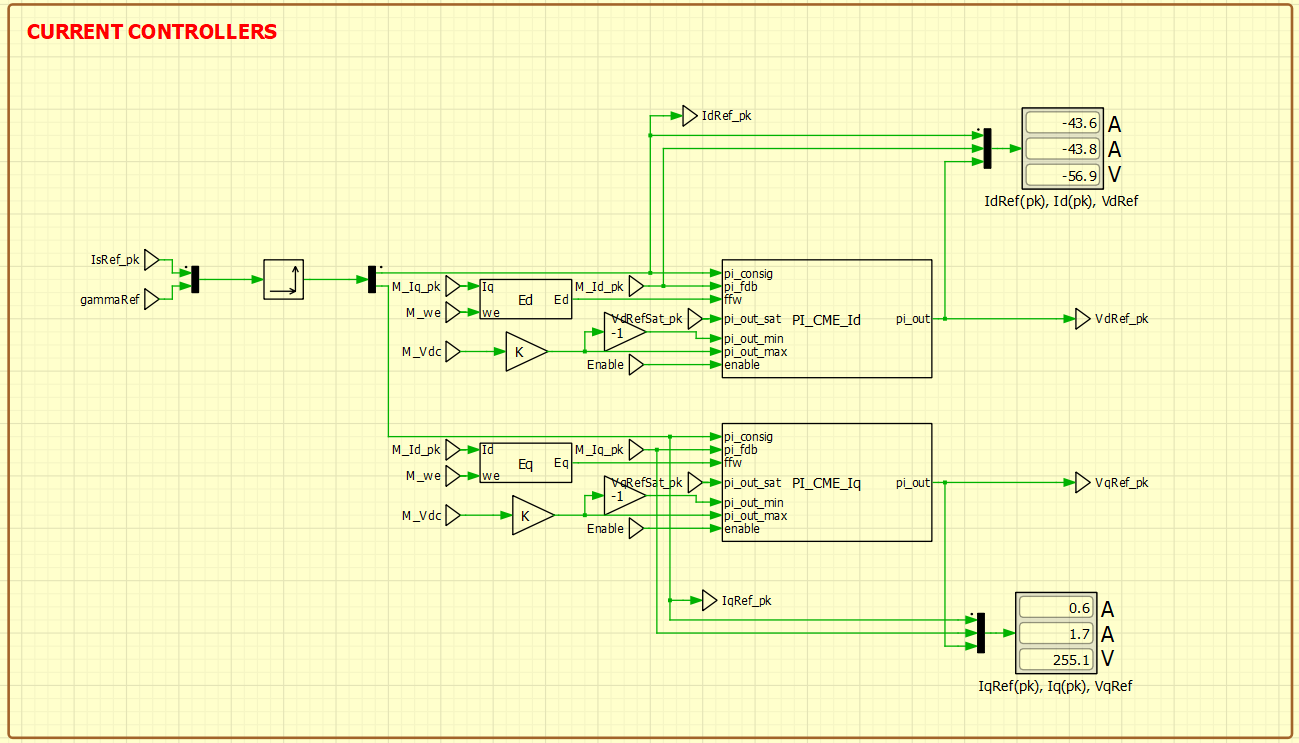
\includegraphics[width=0.7\linewidth]{fig/PLECS_current-loop}
	\caption{Los lazos de corriente están implementados con PIs discretos de la librería PERGAMON y afinados analíticamente con el procedimiento mostrado anteriormente.}
\end{figure}
\begin{figure}[H]
	\centering
	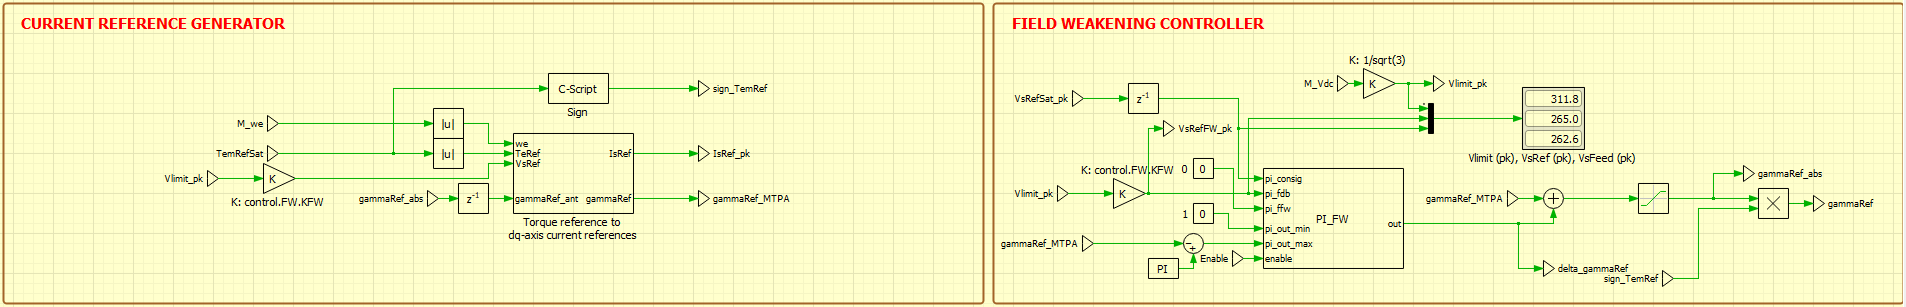
\includegraphics[width=0.9\linewidth]{fig/PLECS_currentref}
	\caption{Consigna de corriente con debilitamiento de campo.}
\end{figure}
\begin{figure}[H]
	\centering
	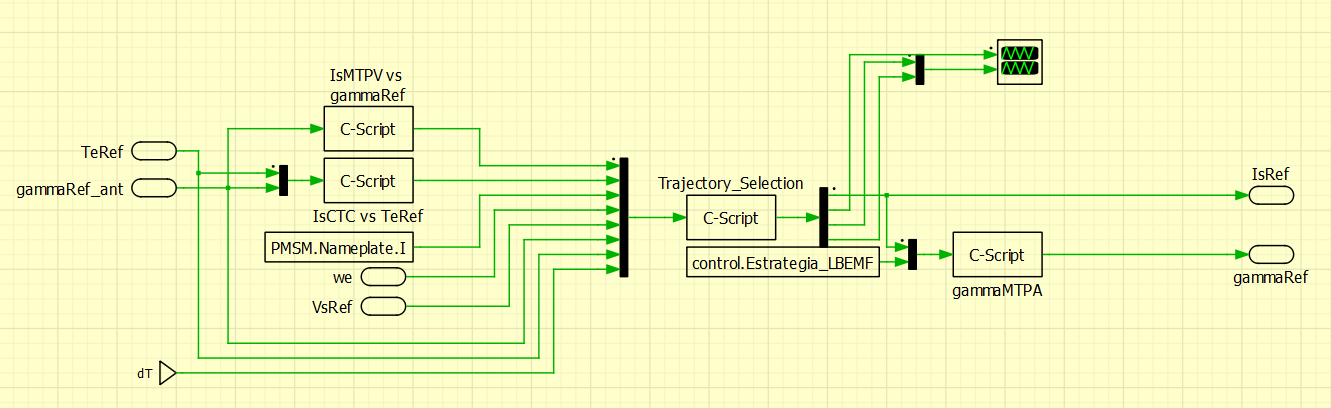
\includegraphics[width=0.7\linewidth]{fig/PLECS_currentref1}
	\caption{Detalle del bloque de cálculo de corriente, donde se implementan las trayectorias de control del PMSM como ecuaciones analíticas resueltas.}
\end{figure}
\begin{figure}[H]
	\centering
	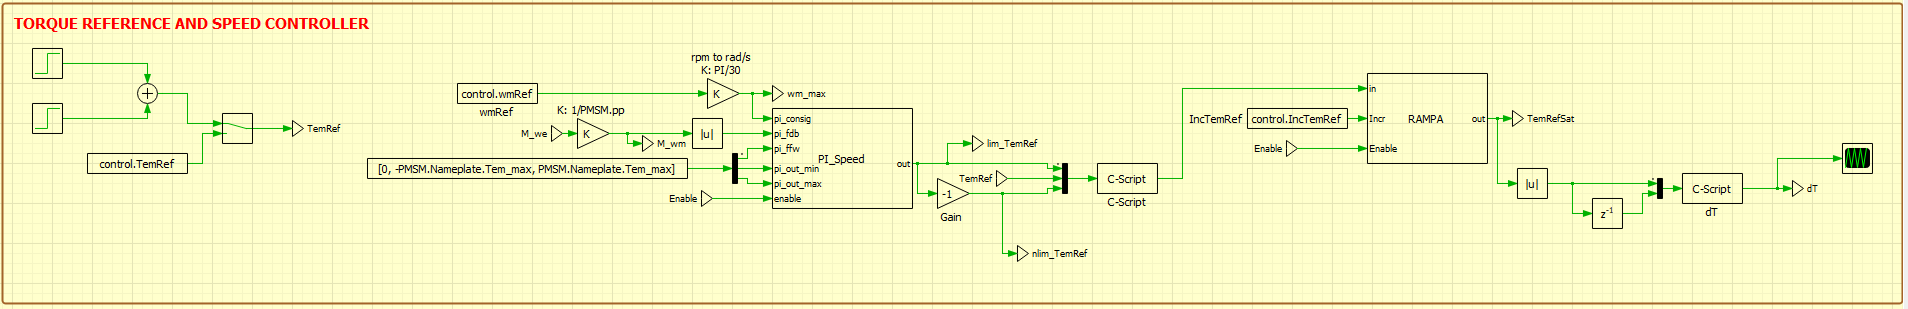
\includegraphics[width=0.9\linewidth]{fig/PLECS_tqspeed}
	\caption{Consigna de par y lazo de velocidad como saturación de la consigna de par.}
\end{figure}
\begin{figure}[H]
	\centering
	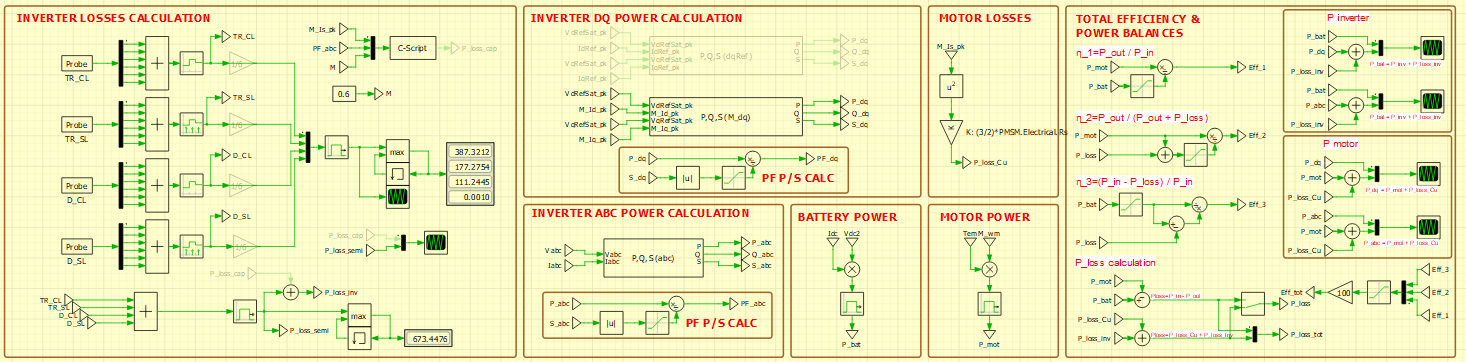
\includegraphics[width=0.7\linewidth]{fig/PLECS_losses}
	\caption{Cálculo de pérdidas, eficiencia y factor de potencia.}
\end{figure}
\begin{figure}[H]
	\centering
	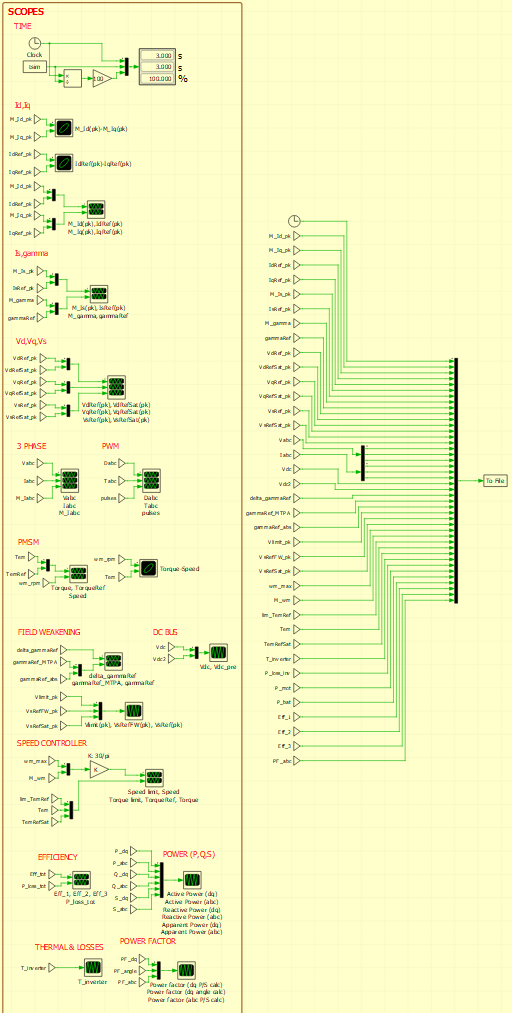
\includegraphics[width=0.4\linewidth]{fig/PLECS_scopes}
	\caption{Visualización y registro de las variables de interés para el análisis y el procesamiento de datos.}
\end{figure}

\begin{figure}[H]
    \centering

    \begin{subfigure}{0.4\textwidth}
        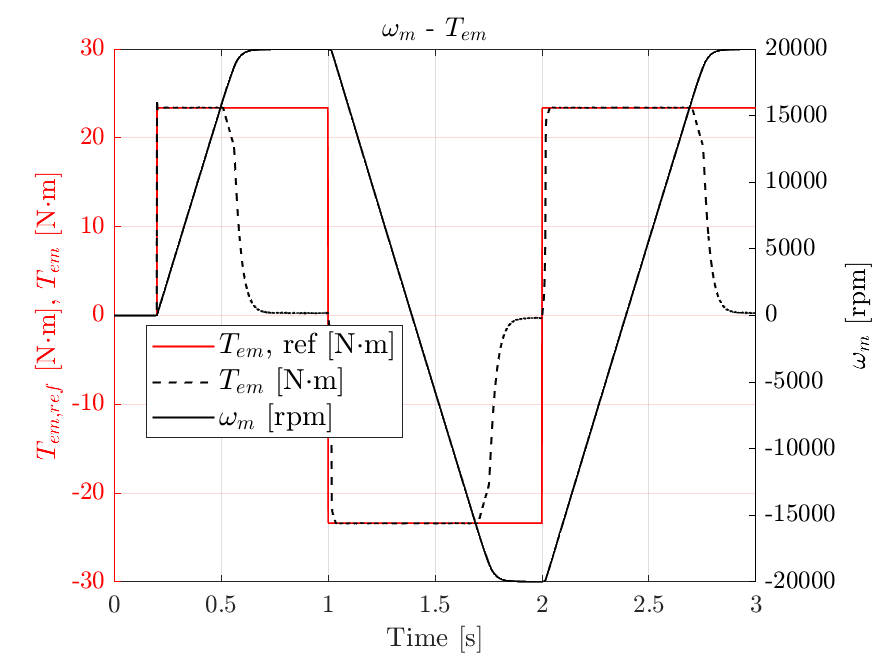
\includegraphics[width=\linewidth]{fig/PLECS_Tem.png}
        \caption{Torque electromagnético ($T_{em}$) y Velocidad mecánica ($\omega_{m}$).}
    \end{subfigure}
    %
    \begin{subfigure}{0.4\textwidth}
        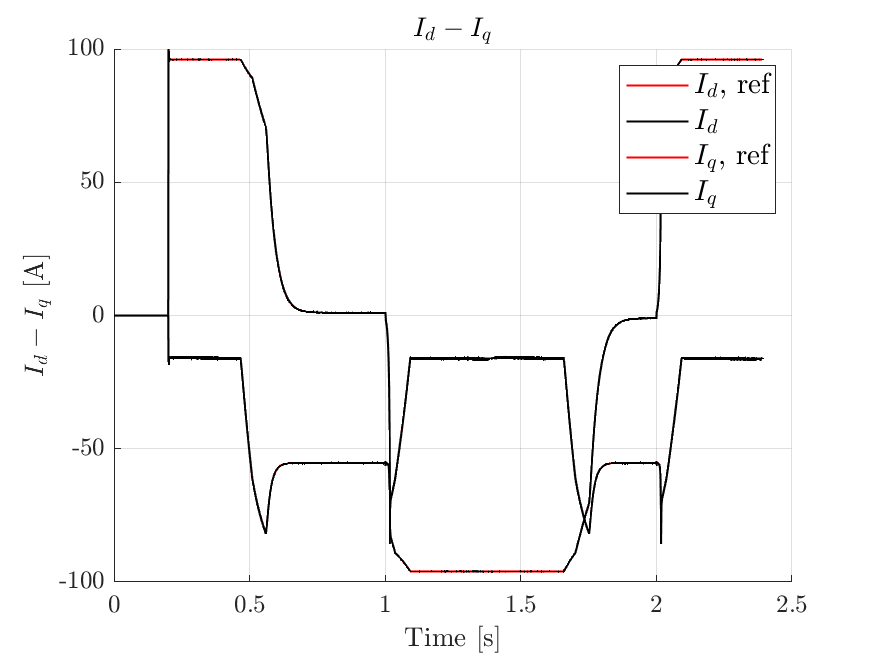
\includegraphics[width=\linewidth]{fig/PLECS_idiq.png}
        \caption{Corrientes ($I_{d} - I_{q}$).}
    \end{subfigure}

    \begin{subfigure}{0.4\textwidth}
        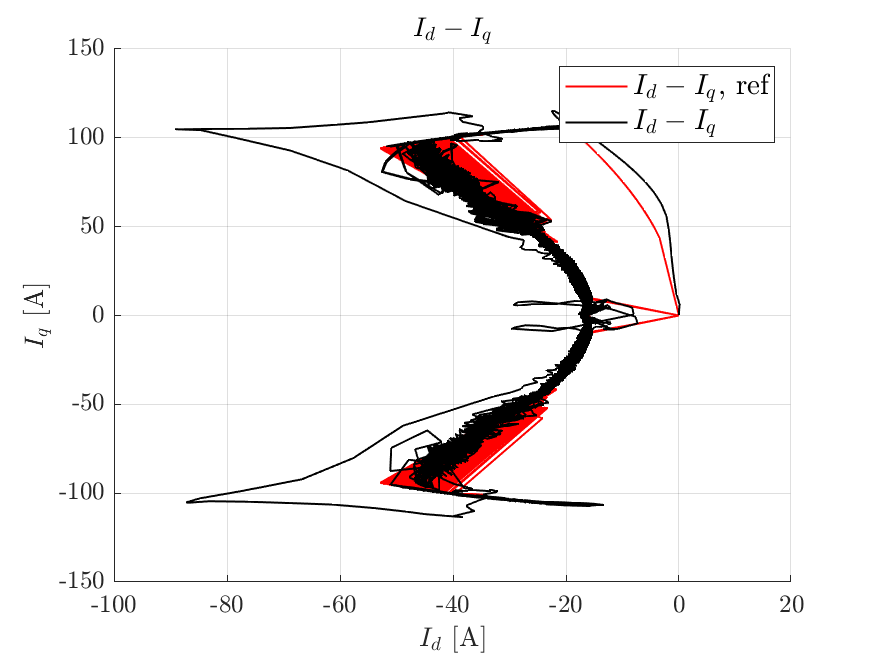
\includegraphics[width=\linewidth]{fig/PLECS_id-iq.png}
        \caption{Corriente ($I_{d}$) vs Corriente ($I_{q}$).}
    \end{subfigure}
    %
    \begin{subfigure}{0.4\textwidth}
        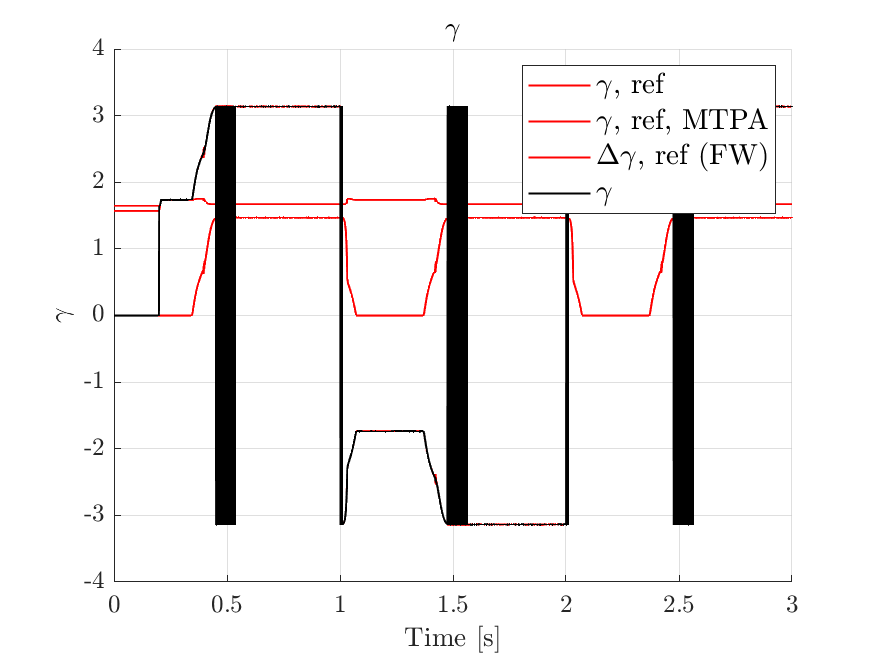
\includegraphics[width=\linewidth]{fig/PLECS_gamma.png}
        \caption{Ángulo de corriente ($\gamma$).}
    \end{subfigure}

    \begin{subfigure}{0.4\textwidth}
        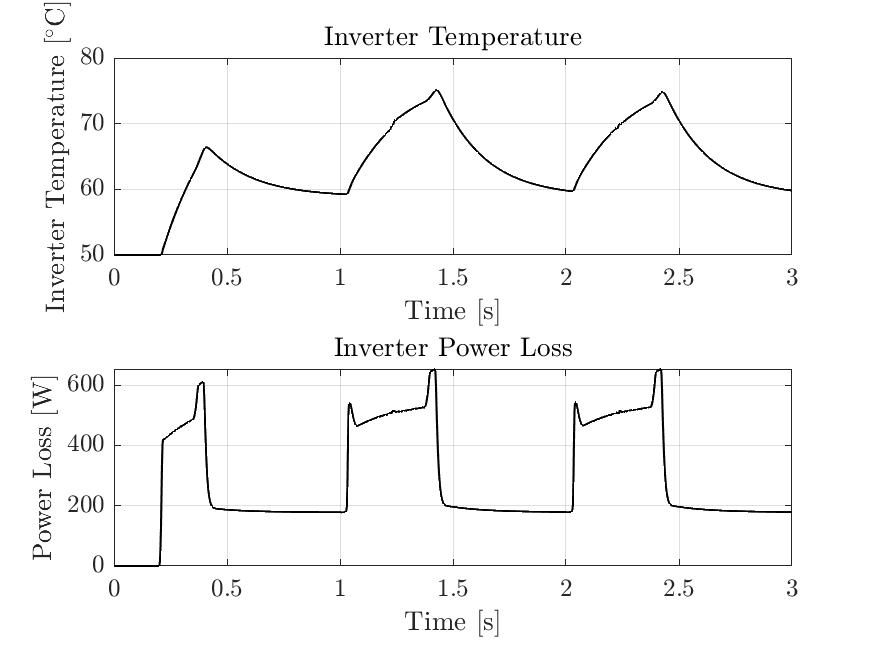
\includegraphics[width=\linewidth]{fig/PLECS_thermal.png}
        \caption{Temperatura y pérdidas del inversor.}
    \end{subfigure}
    %
    \begin{subfigure}{0.4\textwidth}
        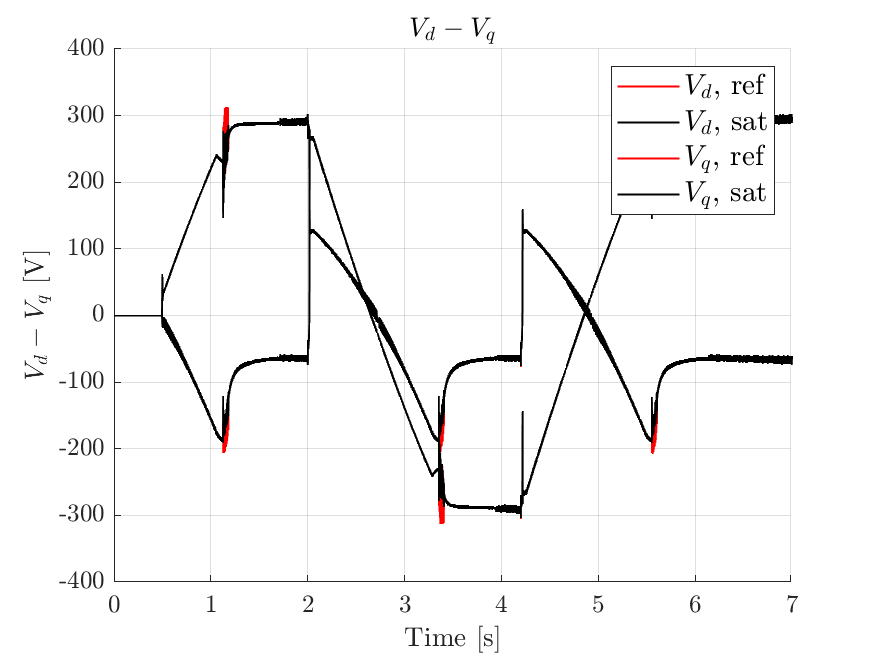
\includegraphics[width=\linewidth]{fig/PLECS_vdvq.png}
        \caption{Voltajes ($V_{d} - V_{q}$).}
    \end{subfigure}

    \caption{Resultados de la simulación.}
\end{figure}

Como se puede observar, se ha optado por consignar un escalón de par del 90\% del par máximo hasta llegar a la velocidad máxima, donde el mismo control es capaz de limitarla. Posteriormente, se consigna un escalón de par igual pero de signo opuesto, para generar una situación extrema y verificar la robustez del control. De esta manera, se evalúa el comportamiento del control vectorial en las circunstancias más adversas, así como el rendimiento teórico del inversor a potencia máxima.

Destaca la claridad con la que esta simulación permite apreciar las trayectorias de control en la figura (c), que muestra la consigna y el valor medido de $i_d$ e $i_q$.



\section{\textit{Hardware}}

\subsection{Requisitos y pre-concepto}

Para definir los requisitos del inversor de tracción, es crucial considerar las restricciones y exigencias del tren de potencia que impone la normativa de la competición, así como los parámetros eléctricos del vehículo en particular en el cual se va a implementar.

\subsubsection{Potencia}
La norma \textit{\textbf{EV2.2.1}} dicta que la potencia en la salida de la batería no debe exceder los 80 kW. Esta restricción es crucial en el diseño del inversor, ya que se prevé que el vehículo sea impulsado por un solo convertidor con esta potencia máxima. Por ende, el inversor debe estar dimensionado para manejar máximos de potencia de hasta 80 kW. Dado que se trata de un inversor doble, la asignación de potencia se divide en 40 kW por motor, aunque se podría necesitar más potencia en uno de los motores durante la aceleración en una curva. Esta decisión se toma pensando en el futuro del equipo, cuando implemente 4 motores, lo que dotaría al vehículo de hasta 160 kW de máximo. Sin embargo, en ese escenario, solo se podrían utilizar 80 kW repartidos entre las 4 ruedas, con un máximo de 40 kW por rueda.

La prueba donde se espera utilizar esta potencia máxima es la \textit{Acceleration}, donde se podría requerir de los 80 kW durante un máximo de 10 segundos, siendo esta una aproximación muy conservadora. Por lo tanto, la potencia máxima queda como:

\(P_{out, max, tot} = 80 \text{kW} (2 \cdot 40 \text{kW}) \text{(10s máx.)}\)


Por otro lado, el requisito de potencia media es distinto. Sería un error dimensionar la potencia media del inversor como el valor máximo, ya que esto conduciría a un sobredimensionamiento excesivo de la refrigeración, los conductores, los conectores y los dispositivos de potencia. En cambio, se opta por determinar el valor medio de potencia requerido durante la prueba más exigente, la \textit{Endurance}. En esta prueba, el vehículo debe recorrer aproximadamente 22 km, lo que equivale a alrededor de media hora de uso continuo. En la \textit{Endurance}, considerar la frenada regenerativa es esencial, ya que aumenta el valor medio de la potencia total, sumándose a la potencia de tracción. Se ha calculado el valor medio de potencia a partir de una simulación de la \textit{Endurance} que llega a máximos de 80 kW:

\begin{figure}[H]
	\centering
	\begin{subfigure}[b]{0.45\textwidth}
		\centering
		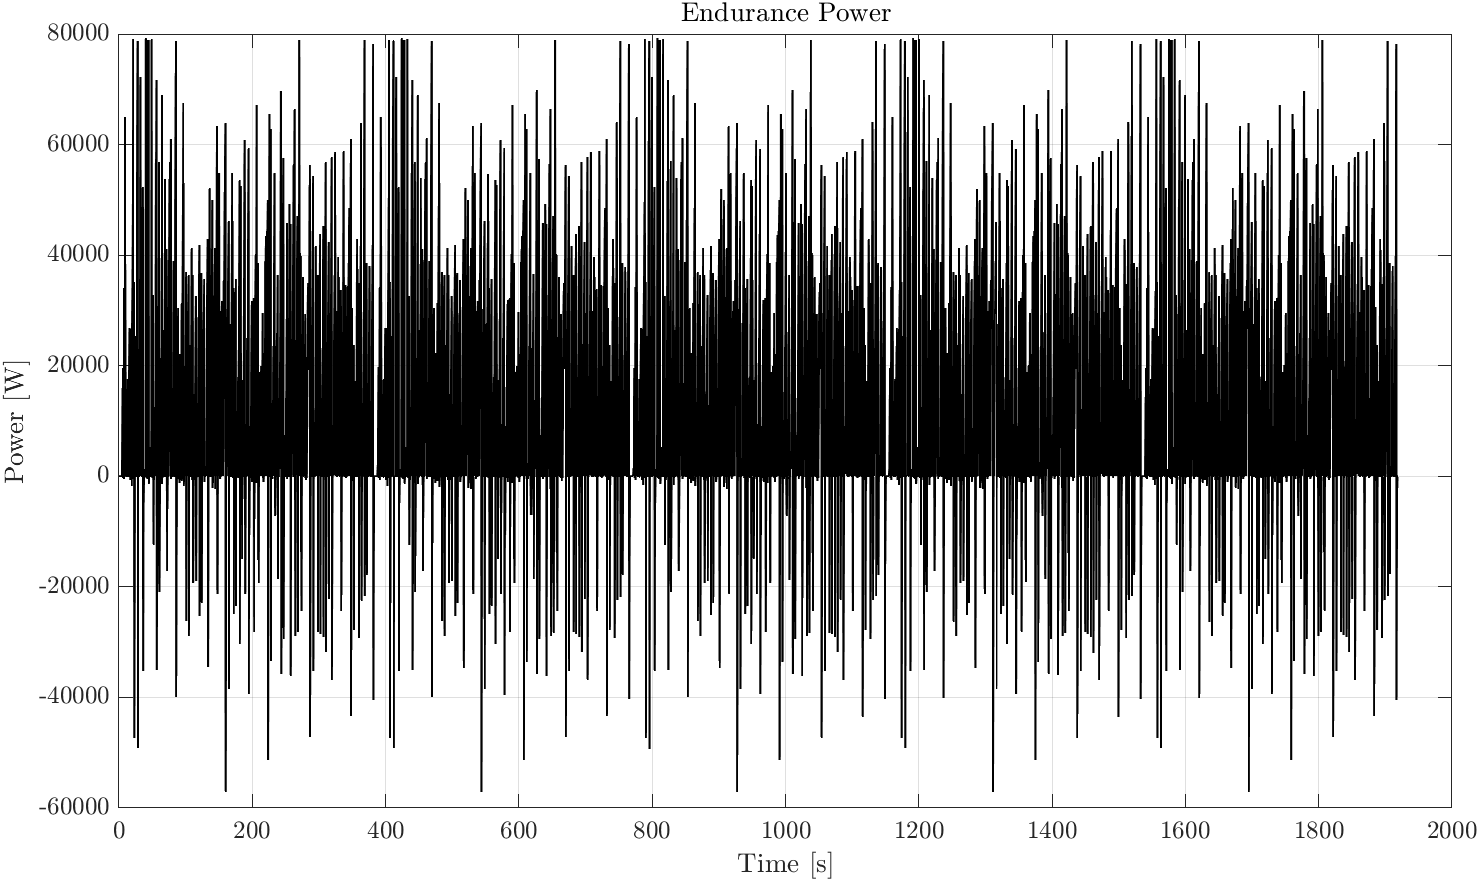
\includegraphics[width=\textwidth]{fig/powerRMS}
	\end{subfigure}
	\hfill
	\begin{subfigure}[b]{0.45\textwidth}
		\centering
		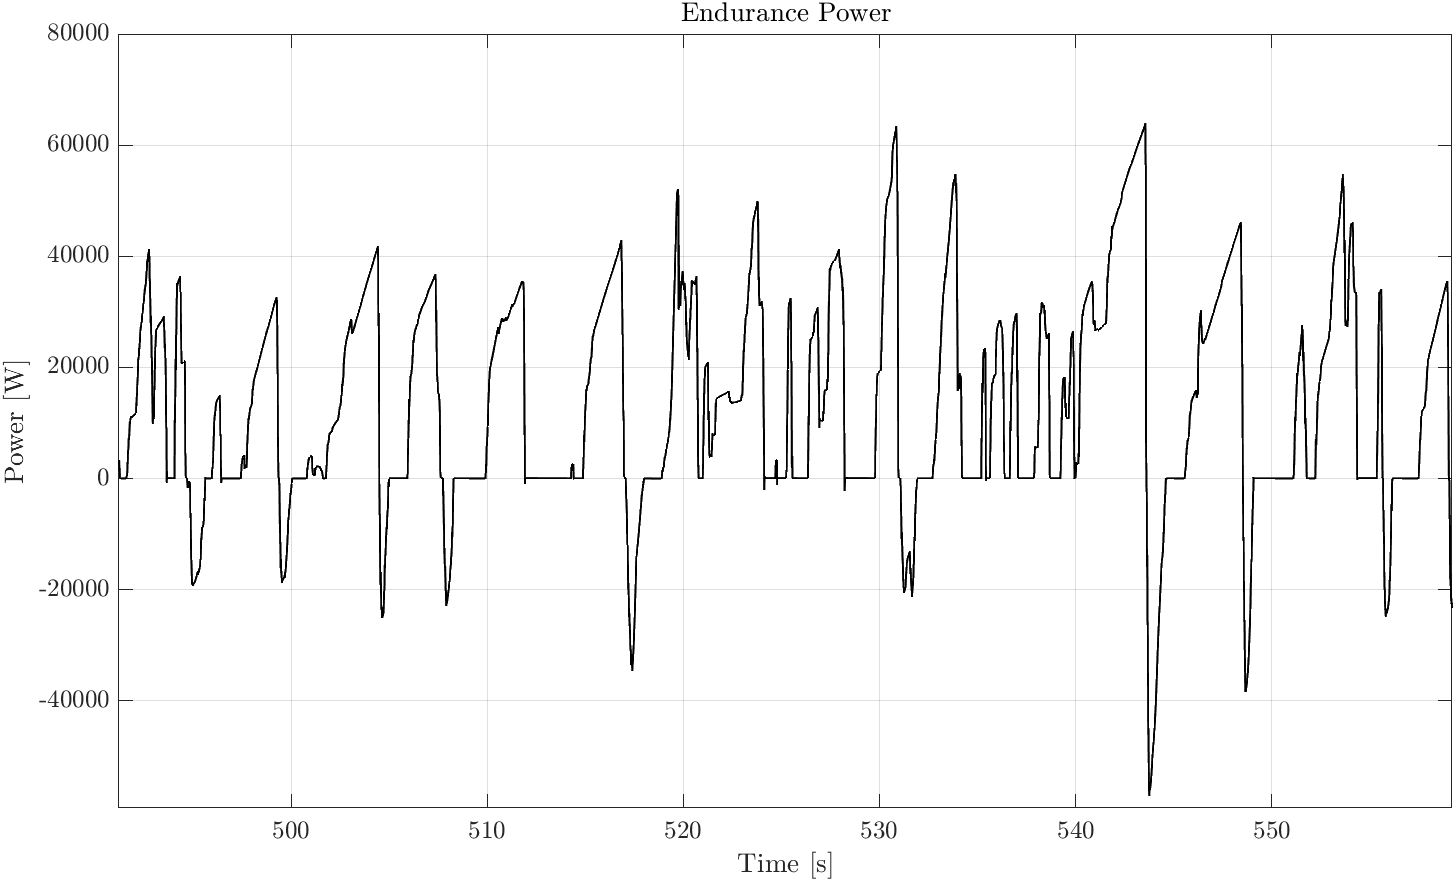
\includegraphics[width=\textwidth]{fig/powerRMS-zoom}
	\end{subfigure}
	\caption{Potencia instantánea que sale de la batería en un evento de \textit{Endurance} (Tiempo completo y detalle de un fragmento).}
\end{figure}

A continuación se muestra el cálculo del valor RMS de la potencia requerida, basado en los datos de potencia:

\begin{verbatim}
	% Calcular el cuadrado de los valores de potencia
	power_squared = power_time.Data.^2;
	
	% Calcular el promedio de los valores cuadrados
	mean_power_squared = mean(power_squared);
	
	% Tomar la raíz cuadrada del promedio de los valores cuadrados para obtener el valor RMS
	power_rms = sqrt(mean_power_squared);
	
	power_rms =
	
	2.3193e+04
\end{verbatim}


Esto demuestra que el valor medio de potencia requerido es considerablemente menor que el pico máximo, en concreto un \(\frac{23.2 \text{kW}}{80 \text{kW}} = 29\%\). Por lo tanto, se dimensiona el inversor considerando una potencia media de 35 kW, es decir, 17.5 kW por motor. Esta cifra proporciona un margen de seguridad de 11.8 kW respecto a la simulación, lo que permite algo de juego en el reparto de potencia entre ambos motores. De esta manera, la potencia constante queda como:

\(P_{out, const, tot} = 35 \text{kW} (2 \cdot 17.5 \text{kW})\)

Cabe destacar que se está calculando la potencia aparente del convertidor, ya que la potencia activa y la reactiva se reparten en función del factor de potencia, que no es constante y depende de la planta mecánica y la situación del motor. La potencia activa es la que usa el motor para acelerar o frenar, y la reactiva la consume o suministra el DC-link. Otra nota es que la simulación es poco realista puesto que utiliza picos de potencia máxima, cuando en realidad, en la prueba de la \textit{Endurance} se suele limitar el valor de estos picos con tal de extender la autonomía.

Además, existe la norma \textit{\textbf{EV4.1.1} The maximum permitted voltage that may occur between any two electrical connections is 600 VDC and for motor controller/inverters internal low power control signals 630 VDC.}, que impone el límite de 600 V para la tensión de bus máxima. Es de interés que el inversor esté dimensionado a esta tensión de funcionamiento, 600 VDC, para permitir máxima flexibilidad con el diseño de la batería, por ejemplo. Al usar la tensión más alta posible, se obtiene un beneficio en la reducción de la corriente, que implica menos pérdidas en los conductores y permite reducir la sección de cables, pletinas, conectores y otros conductores.

Ya que la estrategia de modulación es SVPWM y la tensión máxima es de 600 V, la tensión alterna fase-neutro de un motor se expresa como:

\(V_{ph-n, pico, 600 VDC} = \frac{V_{DC}}{\sqrt{3}} = \frac{600 \text{V}}{\sqrt{3}} = 346 \text{V}\)

\(V_{ph-n, RMS, 600 VDC} = \frac{V_{ph-n, pico}}{\sqrt{2}} = \frac{346 \text{V}}{\sqrt{2}} = 245 \text{V}\)

Sin embargo, la batería no estará constantemente a 600 VDC, por lo que para poder entregar la potencia de 40 kW pico por inversor en un rango de tensiones adecuado se debería calcular la corriente con una tensión menor. Se escoge 450 VDC como tensión mínima a partir de la cual se puede entregar la potencia máxima de 40 kW por inversor. Entonces, la corriente de fase de un motor queda:

\(V_{ph-n, pico, 450 VDC} = \frac{V_{DC}}{\sqrt{3}} = \frac{450 \text{V}}{\sqrt{3}} = 261 \text{V}\)

\(V_{ph-n, RMS, 450 VDC} = \frac{V_{ph-n, pico}}{\sqrt{2}} = \frac{261 \text{V}}{\sqrt{2}} = 184 \text{V}\)


\(I_{ph, RMS, max} = \frac{P_{out, max}}{3\cdot V_{ph-n, RMS, 450 VDC}} = \frac{40 \text{kW}}{3\cdot184 \text{V}} = 72 \text{A}\)

\(I_{ph, pico, max} = I_{ph, RMS, max}\cdot\sqrt{2} = 72\text{A} \cdot\sqrt{2} = 102 \text{A}\)

De la misma manera que con la potencia, se puede obtener el valor de corriente constante a una tensión menor, ya que el resultado será más restrictivo:

\(I_{ph, RMS, const} = \frac{P_{out, const}}{3\cdot V_{ph-n, RMS, 450 VDC}} = \frac{17.5 \text{kW}}{3\cdot184 \text{V}} = 32 \text{A}\)

\(I_{ph, pico, const} = I_{ph, RMS, const}\cdot\sqrt{2} = 32 \text{A}\cdot\sqrt{2} = 45 \text{A}\)


Iterando el cálculo de potencia, se puede ver que si se dimensiona a estas corrientes, las potencias máxima y constante calculadas a 600 VDC son considerablemente mayores:

\(P_{out, max} = 3\cdot V_{ph-n, RMS, 600 VDC}\cdot I_{ph, RMS, max} = 3\cdot245 \text{V}\cdot 72 \text{A} = 53 \text{kW}\)

\(P_{out, const} = 3\cdot V_{ph-n, RMS, 600 VDC}\cdot I_{ph, RMS, const} = 3\cdot245 \text{V}\cdot 32 \text{A} = 23.5 \text{kW}\)

\(P_{out, max, tot} = 2\cdot P_{out, max} = 2\cdot53 \text{kW} = 106 \text{kW}\)

\(P_{out, const, tot} = 2\cdot P_{out, const} = 2\cdot23.5 \text{kW} = 47 \text{kW}\)


\subsubsection{Velocidad}
Puesto que se va a controlar un motor con posibilidad de operación en debilitamiento de campo, es necesario conocer la frecuencia eléctrica máxima que se va a tener que poder sintetizar. Este requisito va a dimensionar la velocidad de los lazos de control, y en última instancia, la frecuencia de conmutación. El motor en estudio tiene 3 pares de polos y una velocidad angular mecánica máxima de 20000 RPM. Por lo tanto, la frecuencia eléctrica máxima que se debe sintetizar se calcula de la siguiente manera:

\(f_{e,max} = \frac{pp\cdot \omega_{m, max, RPM}}{60} = \frac{3\cdot 20000 \text{RPM}}{60} = 1000 \text{Hz}\)

Dejando un poco de margen para la compatibilidad con motores de más polos, se escoge una frecuencia máxima de 1200 Hz. Para sintetizar esta frecuencia eléctrica con poca distorsión armónica, se debe escoger una frecuencia de conmutación al menos 30 veces superior, para tener como mínimo 30 pulsos por periodo a estas frecuencias.

\(f_{\text{conm}} > 30\cdot f_{e,max} = 30\cdot1200 \text{Hz} = 36 \text{kHz} \rightarrow f_{\text{conm}} = 50 \text{kHz}\)

Se debe considerar también que con una frecuencia de conmutación mayor, las pérdidas de conmutación serán más grandes, pero el tamaño del bus de condensadores será más pequeño. Además, el lazo de control debe ir a 50 kHz, con lo que el microcontrolador que lo implemente debe ser capaz de ejecutar todos los cálculos en menos de $\frac{1}{50 \text{kHz}} = 20 \mu\text{s}$.

Es importante que el control sea mucho más rápido que la planta eléctrica, cuya constante de tiempo es de:

\(\text{min}(\frac{L_d}{R_s},\frac{L_q}{R_s}) = \text{min}(\frac{188.7 \mu H}{0.15 \Omega},\frac{283.1 \mu H}{0.15 \Omega}) = \text{min}(1.258 \text{ms}, 1.887 \text{ms}) = 1.258 \text{ms}\)

\(1.258 \text{ms} >> 20 \mu\text{s}\)

\subsubsection{Normativa}
La normativa de la Formula Student no impone normativas muy restrictivas, ya que la mayoría están enfocadas a la seguridad. Estas son las normas que afectarán al diseño del inversor:

\begin{itemize}

    \item \textit{\textbf{EV2.2.2} Regenerating energy is allowed and unrestricted.} La posibilidad de regenerar energía implica que el inversor debe ser capaz de consignar par en el sentido opuesto a la velocidad de los motores para frenar, lo que tendrá un impacto fundamental en el diseño del control. La topología de VSI es bidireccional en sí misma.
    \item \textit{\textbf{EV2.2.3} Wheels must not be spun in reverse.} Podría impactar la lógica de control del inversor y en la adquisición de los sensores de posición para evitar la marcha atrás. Se pueden implementar algoritmos de dependencia de dirección para que ambos motores traccionen el vehículo en la misma dirección.
    \item \begin{itquote} \textbf{EV3.1.1} TS enclosures, see EV1.1.2, must consist of either
    \begin{itemize}
            \item a grounded solid layer made of at least 0.5 mm thick electrically conductive material, aluminium or better, having a resistance below 300 m$\Omega$, measured with a current of 1 A, to LVS ground and able to continuously carry at least 10\% of the TS accumulator main fuse current rating or 
            \item be fully made out of electrically insulating materials having an isolation resistance of at least 2 M$\Omega$, measured with a voltage of 500 V. The enclosure must be rigid and must prevent possible mechanical penetrations. Protruding electrically conductive parts, such as fasteners or connectors, must follow EV3.1.2
    \end{itemize} The TSAC might use at least 0.9 mm thick steel layer as the grounded layer. \end{itquote} Tendrá efectos en el diseño del empaquetado del convertidor y en la selección de materiales para garantizar la seguridad eléctrica y mecánica del convertidor.

    \item \textit{\textbf{EV3.2.5} All overcurrent protection devices that are part of the TS must not rely on programmable logic. The overcurrent protection function of motor controllers/inverters for the motor outputs may rely on programmable logic.} Los dispositivos de protección contra sobrecorriente en el sistema de tracción para el motor pueden depender de lógica programable, lo que permite utilizar el sensado de corriente para garantizar esta protección.
    \item \textit{\textbf{EV4.1.2} All components in the TS must be rated for the maximum TS voltage. The TS area of a PCB, see EV4.3.6, is considered as one component. Every input connected to the TS must be rated to the maximum TS voltage.} Tendrá efectos en la selección de los componentes del circuito de potencia del inversor.
    \item \textit{\textbf{EV4.1.3}  All components must be rated for the maximum possible temperature that may occur during usage.} Impactará en la selección de componentes que puedan manejar las temperaturas esperadas.
    \item \textit{\textbf{EV4.2.1} TS enclosures, see EV1.1.2, must be labeled with (a) reasonably sized sticker(s) according to “ISO 7010-W012” (triangle with a black lightning bolt on a yellow background). The sticker must also contain the text “High Voltage” if the voltage is more than 60 VDC or 50 VACRMS.} Impacta en los requisitos de señalización y seguridad del empaquetado.
    \item \textit{\textbf{EV4.3.1} The entire TS and LVS must be galvanically isolated, see EV1.2.1 and IN4.1.1.} Afecta el diseño de la separación y el aislamiento entre ambos sistemas.
    \item \textit{\textbf{EV4.3.4} Where both TS and LVS are present within an enclosure, they must be separated by barriers made of moisture-resistant insulating materials or maintain the following spacing through the air, or over a surface:}

	\begin{table}[H]
		\centering
		\caption{Voltage Spacing Requirements}
		\begin{tabular}{|l|l|}
			\hline
			Voltage         & Spacing     \\ \hline
			\(U < 100 \text{VDC}\)  & 10 mm       \\ \hline
			\(100 \text{VDC} < U < 200 \text{VDC}\) & 20 mm       \\ \hline
			\(U > 200 \text{VDC}\)  & 30 mm       \\ \hline
		\end{tabular}
	\end{table} Impacta en el diseño del empaquetado del inversor.  Se usarán aislantes como el Nomex en caso de que no se pueda garantizar el espaciado por aire.
    \item \textit{\textbf{EV4.3.6} If TS and LVS are on the same PCB, they must be on separate well-defined areas of the board, meeting the spacing requirements in table 5, each area clearly marked with “TS” or “LV”. The outline of the area required for spacing must  be marked. “Conformal coating” refers to a coating insulator, solder resist is not a coating.}
    
	\begin{table}[H]
		\centering
		\caption{Voltage Spacing Requirements}
		\begin{tabular}{|l|l|l|l|}
			\hline
			Voltage & Over Surface & Through Air (Cut in board) & Conformal Coating \\
			\hline
			0 to 50 & 1.6 mm & 1.6 mm & 1.0 mm \\
			\hline
			50 to 150 & 6.4 mm & 3.2 mm & 2.0 mm \\
			\hline
			150 to 300 & 9.5 mm & 6.4 mm & 3.0 mm \\
			\hline
			300 to 600 & 12.7 mm & 9.5 mm & 4.0 mm \\
			\hline
		\end{tabular}
	\end{table} Tendrá efectos en el diseño de la PCB de potencia.

    \item \textit{\textbf{EV4.5.3} The temperature rating for TS wiring, connections, and insulation must be appropriate for the expected surrounding temperatures but at least 85 ºC.} Influirá en la selección de cables y materiales aislantes.
    \item \textit{\textbf{EV4.5.4} TS components and containers must be protected from moisture in the form of rain or puddles, see IN9.} Impactará en el diseño de la caja.
    \item \textit{\textbf{EV4.5.6} All TS wiring must be completed to professional standards with appropriately sized conductors and terminals and with adequate strain relief and protection from loosening due to vibration etc.} Tendrá efectos en el diseño de las conexiones y terminales.
    \item \textit{\textbf{EV4.5.10} Every TS connector outside of a housing must include a pilot contact/interlock line which is part of the SDC. Housings only used to avoid interlocks are prohibited.} Impactará en el diseño de los conectores y sistemas de interconexión.
    \item \textit{\textbf{EV4.5.11} All TS connections must be designed so that they use intentional current paths through conductors such as copper or aluminium and must not rely on steel bolts to be the primary conductor.} Tendrá efectos en el diseño de las conexiones y la selección de materiales adecuados.
    \item \textit{\textbf{EV4.5.12} All TS connections must not include compressible material such as plastic in the stack-up or as a fastener. FR-4 is allowed.} Impactará en el diseño de las conexiones y la selección de materiales adecuados.
    \item \textit{\textbf{EV4.5.13} TS connectors outside of TS enclosures must be designed in a way, that the TS cannot be activated, see EV4.11, if connected in any way other than the design intent configuration.} Tendrá efectos en el diseño de los conectores y la seguridad.
    \item \textit{\textbf{EV4.5.14} All electrical connections, including bolts, nuts, and other fasteners, in the high current path of the TS must be secured from unintentional loosening. Fasteners must use positive locking mechanisms, see T10.2, that are suitable  for high temperatures, see EV4.5.3.} Impactará en el diseño de los sistemas de fijación y bloqueo, especialmente en las conexiones de potencia.
    \item \begin{itquote} \textbf{EV4.5.16} Soldered connections in the high current path are only allowed if all of the following are true: 
    \begin{itemize}
            \item connections on PCBs
            \item the connected devices are not cells or wires
            \item the devices are additionally mechanically secured against loosening
    \end{itemize} \end{itquote} Tendrá efectos en el diseño de las conexiones y el uso de soldaduras. El uso de sistemas alternativos de conexión en placa como el \textit{press-fit}, facilita el cumplimiento de esta norma.
    \item \textit{\textbf{EV4.9.1} If a discharge circuit is required to meet EV6.1.5, it must be designed to handle the maximum TS voltage permanently. After three subsequent discharges within 15 s in total, the discharge time specified in EV6.1.5 may be exceeded.  Full discharging functionality must be given after a reasonable time with a deactivated discharge circuit.} Se deberá integrar un circuito de descarga en el inversor que cumpla con estos requisitos.
    \item \textit{\textbf{EV4.9.2} The discharge circuit must be wired in a way that it is always active whenever the SDC is open. Furthermore, the discharge circuit must be fail-safe such that it still discharges the intermediate circuit capacitors if the HVD has  been opened or the TS accumulator is disconnected.} Tendrá efectos en la implementación del circuito de descarga.
    \item \begin{itquote} \textbf{EV2.2.1} EV4.10.2 The TSAL itself must have a red light, flashing continuously with a frequency between 2 Hz and 5 Hz and a duty cycle of 50\%, active if and only if the LVS is active and the voltage across any DC-link capacitor exceeds 
    \begin{itemize}
            \item 60 VDC or 50 VACRMS
            \item Half the nominal TS voltage
    \end{itemize} 
    whichever is lower \end{itquote} Se deberá implementar esta detección.
    \item \textit{\textbf{EV4.10.4} The mentioned voltage detection must be performed inside the respective TS enclosure.} Obliga a situar la detección de alta tensión en el propio \textit{DC-link}.

\end{itemize}

Estas restricciones no solo definen los límites de diseño del inversor, sino que también influyen en la selección de componentes y la estrategia de control.

\subsubsection{Resumen de Requisitos de \textit{Hardware}}

Con toda la información que se ha recopilado se pueden listar los requisitos más importantes del convertidor:
\begin{itemize}
	\item \textbf{Topología del convertidor:} VSI doble.
	\item \textbf{Potencia pico:} 80 kW ($2\cdot40$ kW).
	\item \textbf{Potencia constante:} 35 kW ($2\cdot17.5$ kW).
	\item \textbf{Tensión DC máxima:} 600 V.
	\item \textbf{Tensión fase-neutro sintetizada máxima:} 245 V,RMS (SVPWM).
	\item \textbf{Corriente de fase máxima:} 80 A,RMS.
	\item \textbf{Aislamiento galvánico entre TS y LVS}.
	\item \textbf{Detección de tensión}.
	\item \textbf{Circuito de descarga integrado}.
	
	
\end{itemize}

\subsubsection{Requisitos Adicionales}
Además de las restricciones normativas, los requisitos del inversor también deben tener en cuenta las demandas específicas del sistema de tracción. Entre estos requisitos se encuentran:

\begin{itemize}
	\item \textbf{Densidad de Potencia:} El inversor debe ser capaz de proporcionar una alta densidad de potencia para facilitar la integración en el vehículo.
	\item \textbf{Eficiencia:} Se busca una eficiencia óptima para maximizar la autonomía del monoplaza y llevar el máximo de energía de la batería a los neumáticos.
	\item \textbf{Fiabilidad:} Dado el entorno de competición, el inversor debe ser altamente confiable y capaz de operar en las condiciones de una competición, como temperaturas ambientales y humedades altas.
	\item \textbf{Flexibilidad:} El diseño del inversor debe ser lo suficientemente flexible para adaptarse a posibles cambios en el sistema de tracción y comunicación con el vehículo.
	\item \textbf{Facilidad de mantenimiento:} Consideraciones para facilitar el mantenimiento y la reparación en caso de fallos durante la competición.
\end{itemize}

\subsubsection{Boceto del empaquetado}

Antes de entrar en el diseño detallado del convertidor, se realizaron algunos bocetos preliminares para visualizar la disposición de los componentes y planificar la distribución espacial. Estos bocetos iniciales sirven como punto de partida para el diseño final del empaquetado del inversor.

\begin{figure}[H]
	\centering
	\begin{minipage}{0.45\textwidth}
		\centering
		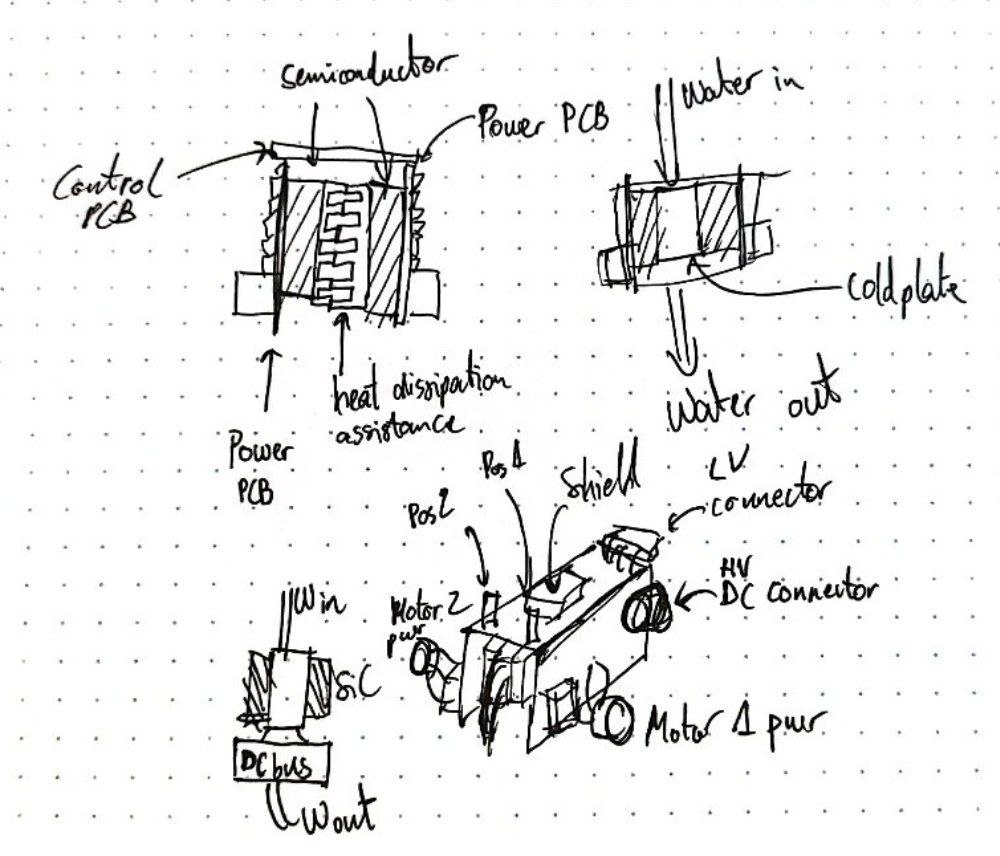
\includegraphics[width=\textwidth]{fig/boceto1}
	\end{minipage}\hfill
	\begin{minipage}{0.45\textwidth}
		\centering
		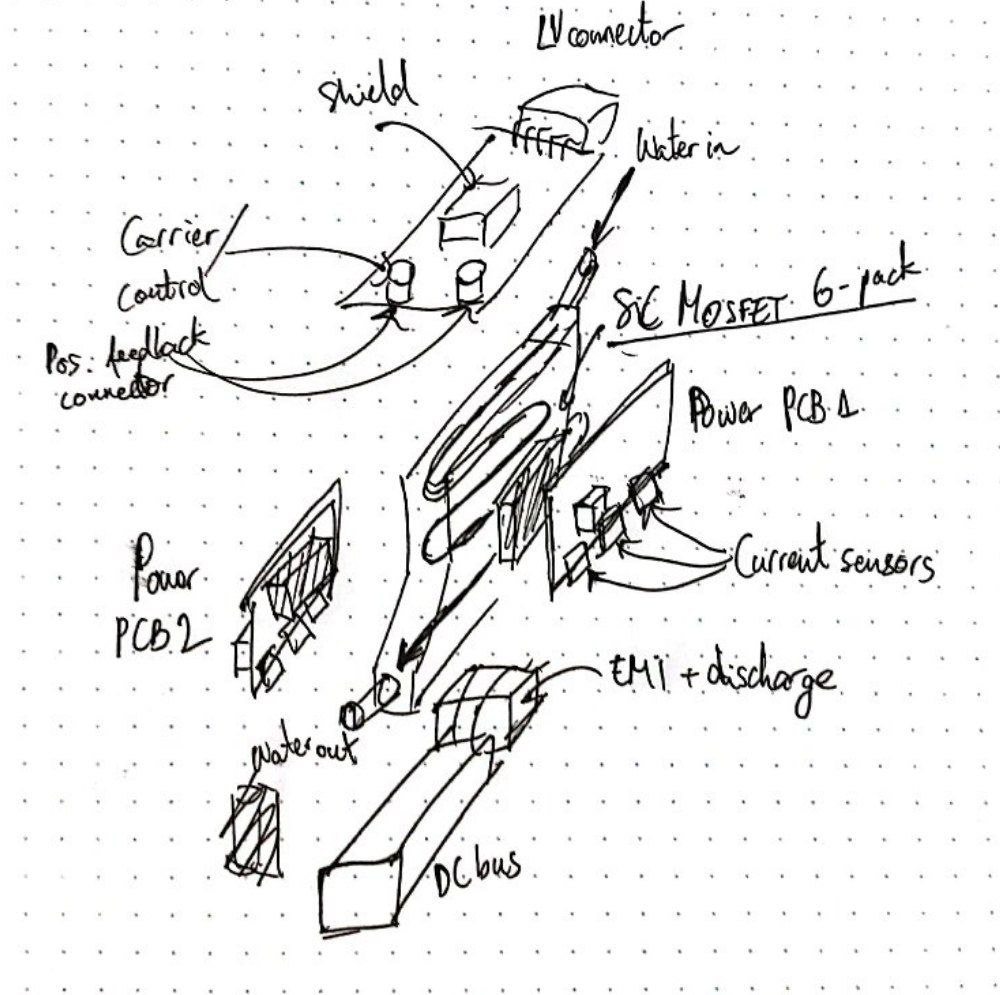
\includegraphics[width=\textwidth]{fig/boceto2}
	\end{minipage}
	\caption{Bocetos preliminares del empaquetado del inversor.}
\end{figure}

En estos dos primeros conceptos se explora el uso de una sola \textit{coldplate} para refrigerar ambos semiconductores. Adicionalmente se propone refrigerar el DC-link, aunque posteriormente se encuentra que no es necesario. Se ha optado por una configuración que separa claramente los módulos de potencia de la placa de control, facilitando así el mantenimiento y la disipación de calor.

\begin{figure}[H]
	\centering
	\begin{minipage}{0.45\textwidth}
		\centering
		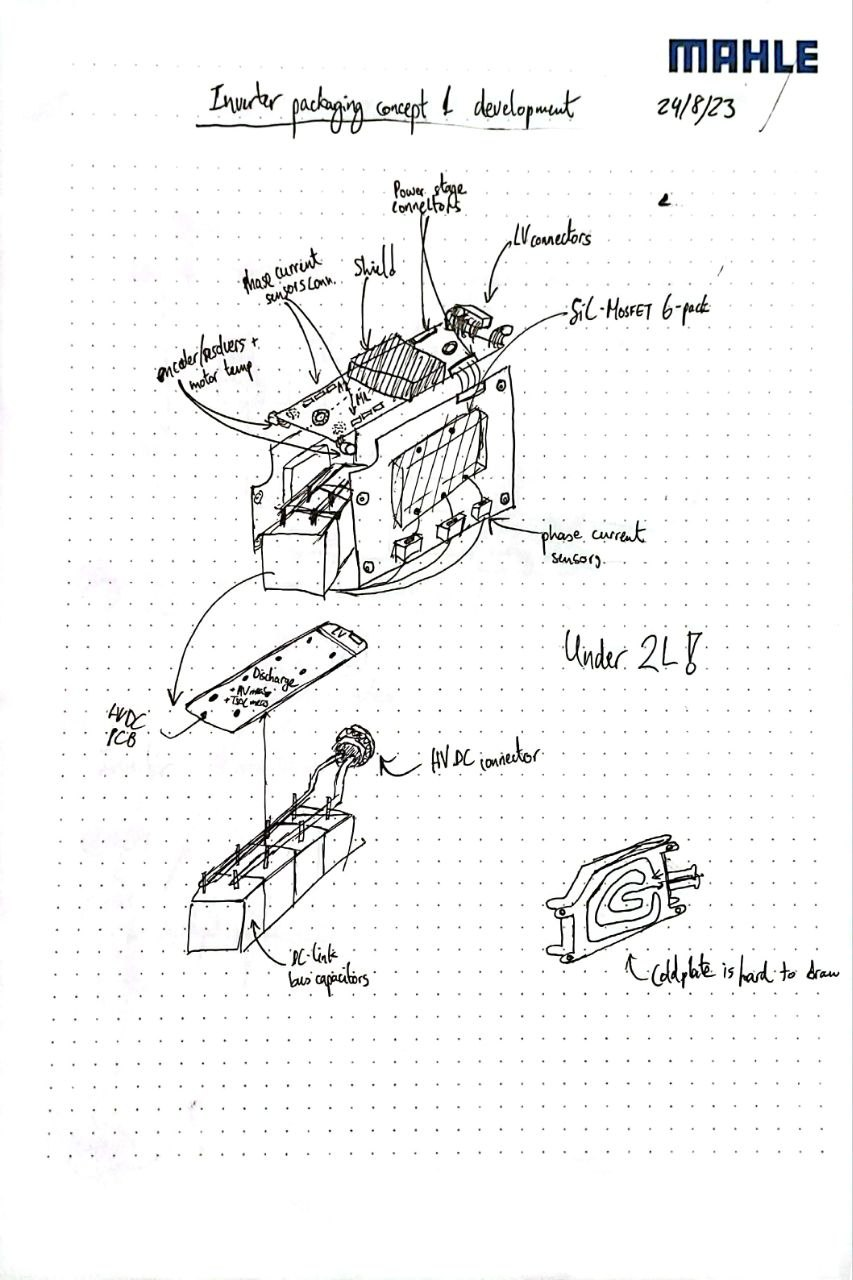
\includegraphics[width=\textwidth]{fig/boceto3}
	\end{minipage}\hfill
	\begin{minipage}{0.45\textwidth}
		\centering
		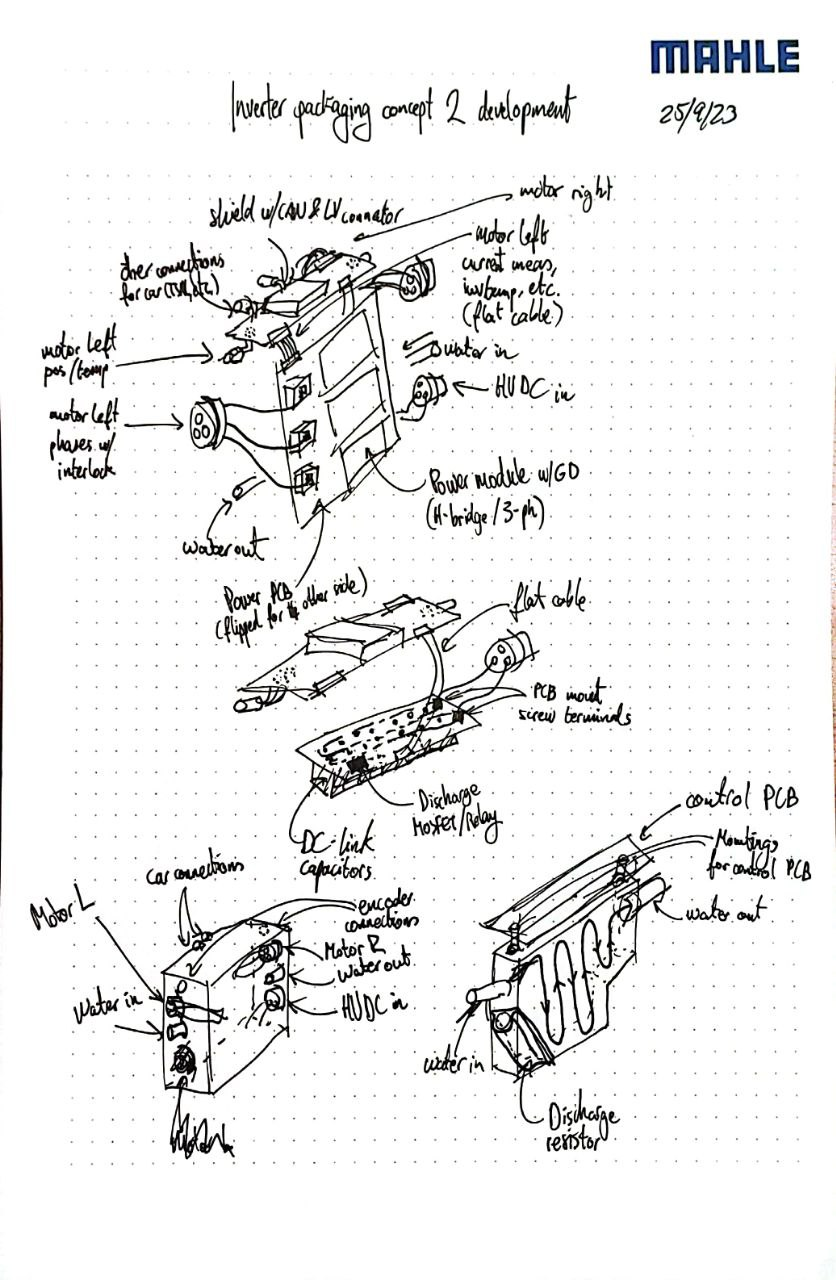
\includegraphics[width=\textwidth]{fig/boceto4}
	\end{minipage}
	\caption{Evolución de los bocetos del empaquetado del inversor.}
	\label{sketches}
\end{figure}

En los bocetos posteriores, se ha refinado la disposición de los componentes para mejorar la accesibilidad y la eficiencia de refrigeración. La disposición de los conectores y la distribución de los conductores también se ha ajustado para optimizar la densidad de potencia y la eficiencia del diseño. Estos cambios reflejan un enfoque hacia un empaquetado más eficiente y funcional del inversor. De todas maneras, todavía presentan muchas complicaciones en el ensamblaje y fabricación de algunos elementos como la \textit{coldplate}.

Estos bocetos iniciales proporcionan una idea visual de cómo se podría organizar el empaquetado del inversor. A medida que avanza el diseño, se realizarán ajustes a la vez que se encuentren limitaciones con los componentes específicos seleccionados y se hagan consideraciones eléctricas y térmicas que en este punto no se han tenido.

\subsection{Topología y concepto}
Con el fin de producir las tensiones trifásicas que calcula el control para los dos motores se implementa un ondulador trifásico fuente de voltaje doble (\textit{dual VSI}). Poniendo el foco en uno solo de los convertidores, existen varias topologías que permiten hacer un ondulador trifásico, pero la más utilizada es el VSI de 2 niveles, formado por tres ramas de medio puente. Otras topologías de más niveles logran sintetizar las tensiones con menos distorsión armónica, pero dado que el motor eléctrico es una carga inductiva, y que el control está basado en consignas de corriente, la distorsión armónica del convertidor tiene un impacto muy poco significativo en el rendimiento global. De esta manera, se justifica la implementación del VSI dual.

\begin{figure}[H]

    \centering
    \begin{circuitikz}
        % Upper MOSFETs
        \draw (0,0) node[nigfete,anchor=D,bodydiode] (M1) {};
        \draw (2,0) node[nigfete,anchor=D,bodydiode] (M2) {};
        \draw (4,0) node[nigfete,anchor=D,bodydiode] (M3) {};

        % Lower MOSFETs
        \draw (0,-2) node[nigfete,anchor=D,bodydiode] (M4) {};
        \draw (2,-2) node[nigfete,anchor=D,bodydiode] (M5) {};
        \draw (4,-2) node[nigfete,anchor=D,bodydiode] (M6) {};

        % Connections
        \draw (M1.S) -- (M4.D);
        \draw (M2.S) -- (M5.D);
        \draw (M3.S) -- (M6.D);
        \draw (M1.D) -- (M2.D) -- (M3.D);
        \draw (M4.S) -- (M5.S) -- (M6.S);

        % Battery
        \draw (M1.D)  |-  ++(-4,0) to[battery, l=$V_{DC}$] ++(0,-3.5)  |-  (M4.S);
        \draw (M1.D)  |-  ++(-1.5,0) to[capacitor] ++(0,-3.5)  |-  (M4.S);

        % Phase cables
        \draw (M3.S)  |-  ++(2,-0.5) node[right, font=\tiny] {C};
        \draw (M2.S)  |-  ++(4,-0.25) node[right, font=\tiny] {B};
        \draw (M1.S)  |-  ++(6,0) node[right, font=\tiny] {A};

    \end{circuitikz}
        \caption{VSI con MOSFETs.}

\end{figure}

Ya que el convertidor implementa código propio, se decide implementar dos VSI en el mismo convertidor, de modo que se opta por unificar algunos elementos de ambos como la refrigeración con el fin de optimizar el peso y el espacio. Esta decisión evita duplicados de medidas, componentes y software, sin embargo, conlleva otros retos, como por ejemplo, que el microcontrolador deberá ser capaz de ejecutar los dos lazos de control al mismo tiempo.

Para adquirir las variables necesarias para el control y la interfaz con el vehículo y sus periféricos, se requieren los submódulos que se presentan en este diagrama de bloques.

\begin{figure}[H]
	\centering
	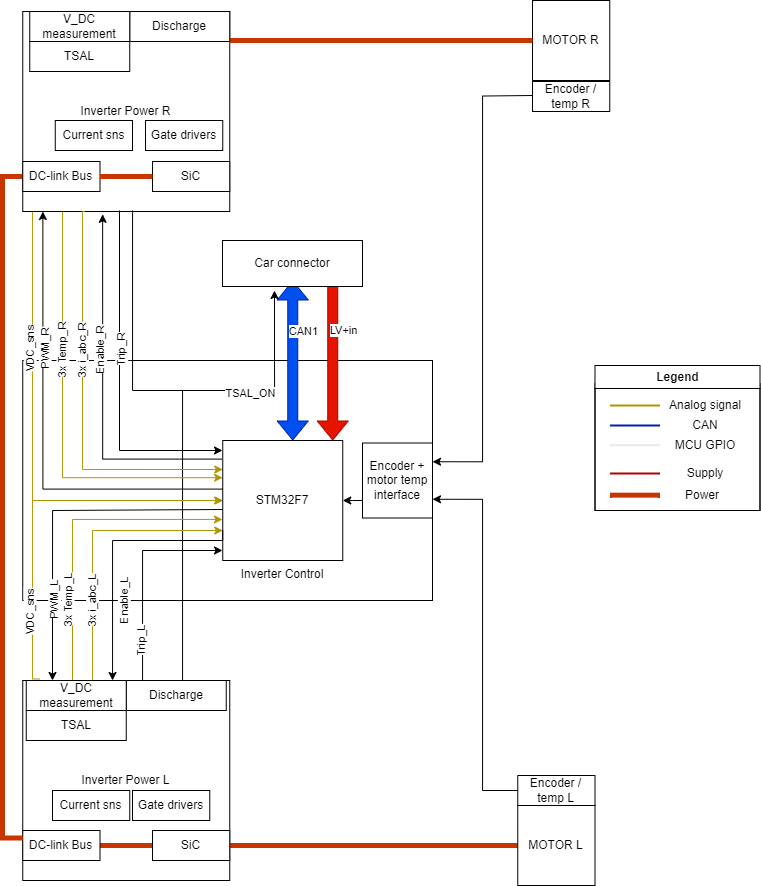
\includegraphics[width=0.7\linewidth]{fig/Inverter_HW}
	\caption{Diagrama de bloques del sistema completo.}
\end{figure}

El convertidor se divide en 3 PCBs, \textit{Inverter Power}, que se instala por duplicado (una por motor), e \textit{Inverter Control}. Como su nombre indica, \textit{Inverter Power} alojará todos los componentes de potencia, incluyendo los \textit{gate drivers}, los sensores de corriente, los semiconductores, los DC-links y los conectores de potencia. Además, en esta placa se puede encontrar el sensado de la tensión de los buses, los circuitos de descarga, y la detección de alta tensión para la \textit{TSAL}. El sensado de tensión sería el único subcircuito repetido, pero esto solamente aporta redundancia y tolerancia al fallo.

Por su parte, \textit{Inverter Control} contiene el microcontrolador de la familia STM32F7 para consignar la conmutación a los \textit{gate drivers}, así como para realizar las lecturas de corriente, tensión y temperatura, las interfaces con los sensores de posición de los motores o los protocolos comunicación CAN y USB.

El montaje de estas placas se realiza de forma compacta y eficiente, de manera que cabe una \textit{coldplate} entre medias de las dos de potencia para refrigerar los semiconductores de ambos inversores. Se encajan de manera que la placa de control se puede conectar a las placas de potencia mediante conectores placa a placa. Las conexiones de potencia facilitan la integración con el cableado del monoplaza debido a su posicionamiento.


\subsection{Semiconductores}

\subsubsection{Tecnología de Semiconductores}

La decisión de emplear MOSFETs de carburo de silicio (SiC) como interruptores se fundamenta en consideraciones específicas de la aplicación y en los requisitos de la competición. En un entorno donde la reducción de peso y volumen es crucial, el SiC emerge como una opción destacada frente a alternativas como el IGBT de silicio, el FET de GaN o el MOSFET de silicio. Aunque que el precio no es una restricción principal en este contexto, el atractivo del proyecto ha logrado captar la atención de empresas que han proporcionado muestras de semiconductores para el desarrollo del convertidor.

Las ventajas inherentes del SiC, como su rendimiento superior o su resistencia a temperaturas más altas, permiten un diseño más compacto y robusto del inversor de tracción. Estas características son esenciales para cumplir con los requisitos de un monoplaza de competición, donde lograr altas densidades de potencia es muy beneficioso para la integración del resto de componentes del vehículo y aligeramiento del mismo.

\subsubsection{Módulos de Potencia}

En el diseño del inversor de tracción, se optó por módulos \textit{half-bridge} debido a su idoneidad para el rango de potencias y tensiones del convertidor. Dos modelos de semiconductores se consideraron para su integración: el DFS05HF12EYR1 de Leapers Semiconductor y el CAB016M12FM3 de Wolfspeed.

Ambos modelos cumplen estrictamente con los requisitos de la aplicación, con un voltaje de ruptura (\(V_{DS,breakdown}\)) de 1200V y una corriente máxima (\(I_{DS,max}\)) que excede los 80 ARMS. La elección de dos modelos distintos se basa en la intención de realizar pruebas comparativas para verificar las diferencias entre ambos.

El DFS05HF12EYR1 ofrece especificaciones muy buenas en su datasheet, aunque Leapers Semiconductors no lleva muchos años en la industria y no han logrado crear la confianza que otras empresas han conseguido con su experiencia. Por otro lado, el CAB016M12FM3, de la reconocida marca Wolfspeed (antiguamente CREE), aporta la confiabilidad asociada a una empresa con amplia experiencia en el campo.

Según sus respectivos datasheets, ambos modelos permiten alcanzar sin mucho esfuerzo una frecuencia de conmutación de 50 kHz, lo que contribuye significativamente a la reducción del tamaño del bus de continua y optimiza el empaquetado del inversor. La placa de potencia se diseñará para permitir la prueba de ambos modelos, ya que comparten \textit{footprint}, facilitando la adaptabilidad y la evaluación comparativa.

A continuación se muestra una tabla comparativa con los detalles de cada semiconductor:
\begin{table}[H]
	\centering
	\begin{tabular}{|l|l|l|}
		\hline
		\textbf{Parámetro} & \textbf{DFS05HF12EYR1} & \textbf{CAB016M12FM3} \\ \hline
		\(V_{DS,\text{breakdown}}\) [V] & 1200 & 1200 \\ \hline
		\(R_{on}\) [\(m \Omega\)] & 5.5 - 13 & 16.0 - 28.8 \\ \hline
		\(V_{f,D}\) [V] & 3.3 - 4 & 4.9 - 5.5 \\ \hline
		\(T_{rr}\) [ns] & 41.5 - 45 & 20.0 \\ \hline
		\(Q_{rr}\) [\(\mu C\)] & 2.19 - 3.94 & 1.30 \\ \hline
		\(R_{th,jc}\) [K/W] & 0.12 - 0.15 & 0.543 \\ \hline
		\(Q_{G}\) [\(nC\)] & 520 & 236 \\ \hline
		\(C_{in}\) [nF] & 14.5 & 6.6 \\ \hline
		\(R_{G,\text{int}}\) [\(\Omega\)] & 1.9 & 2.4 \\ \hline
		\(V_{GS,\text{th}}\) [V] & 2.8 - 4.8 & 1.8 - 3.6 \\ \hline
		\(I_{DS,\text{max}}\) [A] & 150 & 89 \\ \hline
		& 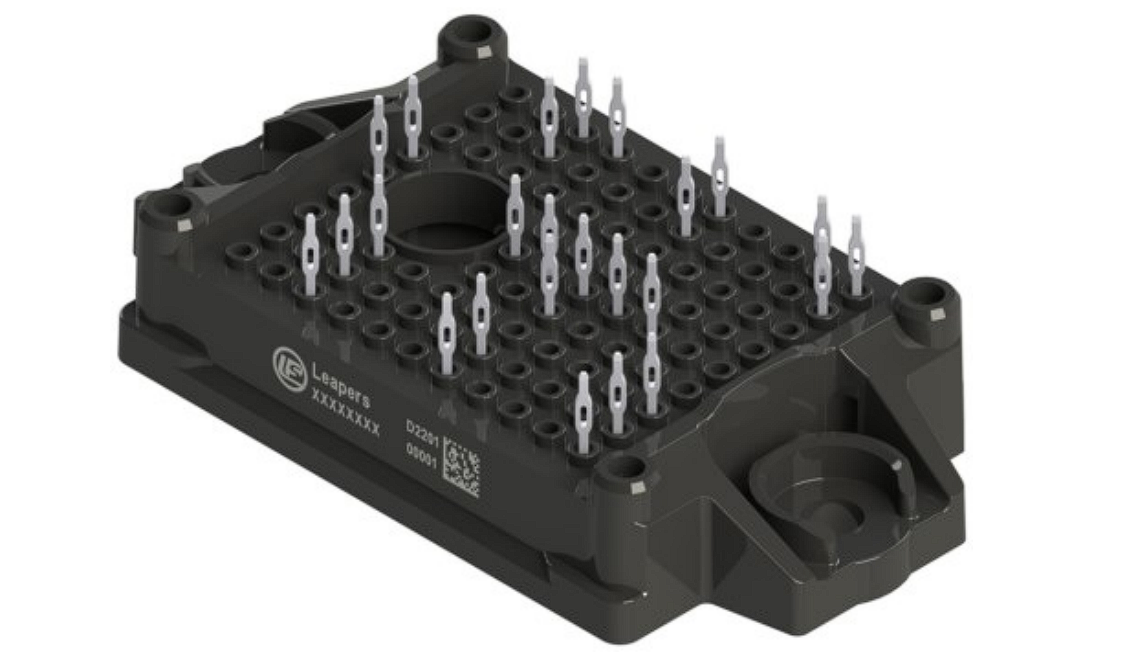
\includegraphics[width=0.2\textwidth]{fig/DFS05.png} & 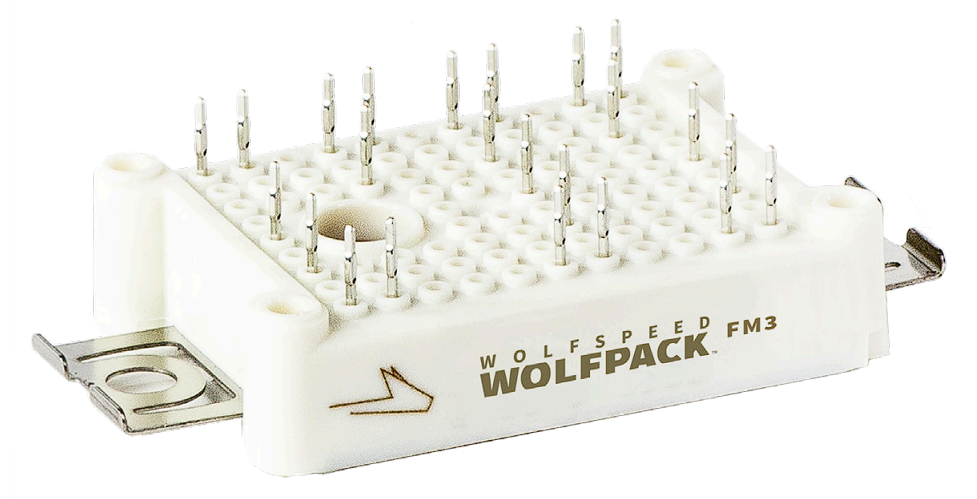
\includegraphics[width=0.2\textwidth]{fig/CAB016.png} \\
		\hline
	\end{tabular}
	\caption{Comparación de parámetros entre DFS05HF12EYR1 y CAB016M12FM3.}
\end{table}

\subsubsection{Análisis de Pérdidas}

Los dispositivos semiconductores experimentan pérdidas de energía que influyen significativamente en su eficiencia y desempeño, y se transforman en calor, limitando así la potencia de salida. Estas pérdidas pueden clasificarse en dos categorías fundamentales: las pérdidas de conducción y las pérdidas de conmutación. Las \textbf{pérdidas de conducción} surgen cuando el dispositivo se encuentra en estado activo, conduciendo corriente a través de él. Esto genera una caída de voltaje y una disipación de potencia asociada a la resistencia interna del dispositivo. Por otro lado, las \textbf{pérdidas de conmutación} se manifiestan durante los ciclos de activación y desactivación del dispositivo, cuando la energía almacenada en la capacitancia del mismo se disipa durante la transición entre los estados de conducción y corte.

En el análisis de la eficiencia de los semiconductores, es imperativo considerar las pérdidas totales, las cuales se definen como la suma de las pérdidas de conducción y las de conmutación:

\begin{equation}
	P_{\text{tot}} = P_{\text{cond}} + P_{\text{conm}}
\end{equation}

A continuación, se examinarán detalladamente las pérdidas de conducción, seguidas por un análisis exhaustivo de las pérdidas de conmutación en los módulos seleccionados.


\textbf{Pérdidas de conducción}

Las pérdidas de conducción tienen su origen en la resistencia entre drenador y fuente cuando el MOSFET está en estado de conducción, o en la caída de tensión del diodo cuando es el diodo quien está conduciendo. Según la ley de Ohm y la definición de potencia:

\begin{equation}
P_{\text{cond,MOSFET}}= I_{DS}^2\cdot R_{DS, on}
\end{equation}

\begin{equation}
P_{\text{cond},D} = I_{SD}\cdot V_f
\end{equation}

Sin embargo, estas expresiones se corresponden con las pérdidas instantáneas y no son útiles a la hora de dimensionar el convertidor. Para ello son necesarias las pérdidas promediadas, pero tienen una expresión analítica muy compleja, ya que dependen de la estrategia de modulación, el índice de modulación instantáneo, el factor de potencia instantáneo, etc. Para el inversor se utiliza SVPWM, pero el cálculo de pérdidas tiene demasiados parámetros instantáneos. Muchas referencias asemejan las pérdidas en SVPWM a las de una modulación PWM sinusoidal (SPWM), con lo que las pérdidas se simplifican y no dependen del desfase entre tensión y corriente $\phi$:

\begin{equation}
P_{\text{cond,MOSFET}} \approx I_{\text{RMS}} V_{Q0} \left(\frac{1}{\pi\sqrt{2}} + \frac{m PF}{2\sqrt{8}}\right) + I_{\text{RMS}}^2 R_Q \left(\frac{1}{4} + \frac{2m}{3\pi PF}\right)
\end{equation}

\begin{equation}
P_{\text{cond},D} \approx I_{\text{RMS}} V_{D0} \left(\frac{1}{\pi\sqrt{2}} - \frac{m PF}{2\sqrt{8}}\right) + I_{\text{RMS}}^2 R_D \left(\frac{1}{4} - \frac{2m}{3\pi PF}\right)
\end{equation}

Como se puede apreciar, aunque son más compactas que otras en la bibliografía, estas expresiones son difíciles de abordar, puesto que casi todos los parámetros son instantáneos. Por ello, se ha usado PLECS para estimar las pérdidas de conducción debido a que facilita la simulación detallada de los semiconductores y permite obtener las pérdidas de forma diseccionada por cada dispositivo y tipo de pérdida. PLECS utiliza modelos detallados de los dispositivos, considerando sus características de conmutación y conducción reales.

Con los parámetros de estos modelos, PLECS calcula las pérdidas de conmutación y conducción de manera precisa. Sin embargo, como no tiene en cuenta el circuito completo de los \textit{gate drivers}, no se pueden tomar directamente las pérdidas de conmutación. Se usa un modelo de MOSFET y diodo de Wolfspeed proporcionado directamente por el fabricante. Este modelo cuenta con una parametrización de las pérdidas y los efectos térmicos mucho más detallada que la que se puede obtener a partir de la hoja de datos. El fabricante utiliza tablas de búsqueda en función de la tensión, corriente y temperatura, e incorpora una relación matemática con las resistencias de puerta. Lamentablemente, Leapers no ofrece esta parametrización con sus semiconductores, por lo que el análisis en PLECS se realiza únicamente con el modelo de Wolfspeed, siendo este el más restrictivo en cuanto a las pérdidas de conducción.

Para sacarle el máximo partido, se ha obtenido un perfil de pérdidas a máxima potencia para el inversor en diferentes zonas de control del PMSM, que se puede observar a continuación.

\begin{figure}[H]
	\centering
	\includegraphics[width=0.9\linewidth]{fig/PLECS-invLosses}
	\caption{Descomposición de las pérdidas de los semiconductores de una simulación en PLECS.}
	\label{losses-sim}
\end{figure}

Se puede ver como las pérdidas de conducción son más significativas que las de conmutación, y varían significativamente. Las zonas de par constante (de 1,05 s a 1,4 s por ejemplo), muestran unas pérdidas casi constantes con la corriente, pero crecen debido a la temperatura. Se anota para una comparación posterior que las pérdidas de conmutación de los MOSFETs están entre 150 y 200 W. Al entrar en la zona de límite de tensión (de 1,4 s a 1,45 s), se observa un pico que se corresponde con la zona de potencia constante, que en esta simulación es la potencia máxima. Para obtener un valor constante de pérdidas con el que diseñar la refrigeración, se parte de este valor de pico (450 W aproximadamente) y se trata de la misma manera que la relación de potencia media respecto a la potencia pico calculada en la sección de requisitos.

\[
\frac{P_{RMS}}{P_{pico}} = \frac{35 kW}{80 kW} = 0.4375 \approx 0.5
\]

Con este razonamiento, se da un valor de pérdidas de conducción máximas de un inversor de $450 \text{W} \cdot 0.5 = 225 \text{W}$. Como hay dos inversores anclados a la misma \textit{coldplate}, las pérdidas de conducción que debe disipar es de $225 \text{W} \cdot 2 = 450 \text{W}$. Es importante recordar que estas pérdidas son para el semiconductor de Wolfspeed. Dado que las pérdidas de conducción son proporcionales a $R_{DS, on}$, se pueden aproximar las pérdidas de conducción del semiconductor de Leapers de la siguiente manera:
\[
P_{\text{cond,Wolfspeed}} = 450 \text{W}
\]

\[
P_{\text{cond,Leapers}} \approx P_{\text{cond,Wolfspeed}} \cdot \frac{R_{DS, on, Leapers}}{R_{DS, on, Wolfspeed}} = 450 \text{W} \cdot \frac{5.5 \text{m}\Omega}{16 \text{m}\Omega} \approx 155 \text{W}
\]


\textbf{Pérdidas de conmutación}

El cálculo de las pérdidas de conmutación es más fácil de determinar de forma analítica, aunque depende del circuito de \textit{gate driver} y de sus parásitos. Si no se tienen en cuenta estos dos factores, se pueden calcular utilizando los valores de \(E_{on}\) y \(E_{off}\), que representan la energía necesaria para encender o apagar el dispositivo respectivamente. Cuando las hojas de datos de los semiconductores proporcionan los valores \(E_{on}\) y \(E_{off}\), las pérdidas de conmutación pueden calcularse de forma directa. Estas pérdidas están influenciadas por la tensión de conmutación, la corriente de conmutación, la temperatura de la unión y la resistencia de puerta. La fórmula comúnmente utilizada para calcular las pérdidas es:

\begin{equation}
E_{conm}(t) = (E_{on} + E_{off}) \left( \frac{I_{Q,env}(t)}{I_{test}} \right)^{K_i} \left( \frac{V_{DC}}{V_{test}} \right)^{K_v}
\end{equation}

Donde \(I_{Q,env}(t)\) es la corriente de conmutación en cada instante de tiempo, \(I_{test}\) y \(V_{test}\) son los valores de prueba, y \(K_i\) y \(K_v\) son coeficientes de ajuste que normalmente son igual a 1. La justificación se puede encontrar en los gráficos proporcionados en las hojas de datos de ambos semiconductores, donde la relación de las energías de encendido y apagado con la corriente son aproximadamente lineales.

\begin{figure}[H]
	\centering
	\begin{subfigure}[b]{0.4\linewidth}
		\centering
		\includegraphics[width=\linewidth]{fig/eoneoffleapers}
		\caption{Leapers}
	\end{subfigure}
	\hfill
	\begin{subfigure}[b]{0.55\linewidth}
		\centering
		\includegraphics[width=\linewidth]{fig/eoneoffwolfspeed}
		\caption{Wolfspeed}
	\end{subfigure}
	\caption{Energías de encendido y apagado en función de la corriente para Leapers y Wolfspeed.}
\end{figure}

Si la corriente es continua, la fórmula simplificada es:

\begin{equation}
P_{conm} \approx (E_{on} + E_{off}) f_{\text{conm}} \frac{I_{out}}{I_{test}} \frac{V_{DC}}{V_{test}}
\end{equation}

Y si la corriente es una sinusoide semi-rectificada con un valor de pico de \(\sqrt{2} I_{rms}\) (como en el caso del SVPWM), la fórmula es:

\begin{equation}
P_{conm} \approx (E_{on} + E_{off}) f_{\text{conm}} \frac{\sqrt{2} I_{rms}}{\pi I_{test}} \frac{V_{DC}}{V_{test}}
\end{equation}

Sustituyendo por los valores del convertidor en diseño:

\begin{itemize}
	\item Generales: \(f_{\text{conm}} = 50 \text{kHz}\), \(I_{\text{rms}} = 80 \text{A}\), \(V_{DC} = 600 \text{V}\)
	\item Leapers: \(E_{\text{on}} = 3.54 \text{mJ}\), \(E_{\text{off}} = 1.59 \text{mJ}\), \(V_{\text{test}} = 600 \text{V}\), \(I_{\text{test}} = 150 \text{A}\)
	\item Wolfspeed: \(E_{\text{on}} = 1.13 \text{mJ}\), \(E_{\text{off}} = 0.54 \text{mJ}\), \(V_{\text{test}} = 600 \text{V}\), \(I_{\text{test}} = 80 \text{A}\)
\end{itemize}

Para los dispositivos Leapers, sustituyendo en la fórmula:

\[
P_{\text{conm, Leapers}} \approx (3.54 \text{mJ} + 1.59 \text{mJ}) \cdot 50 \text{kHz} \cdot \frac{80 \text{A}}{150 \text{A}} \cdot \frac{600 \text{V}}{600 \text{V}} \approx 61.58 \text{W}
\]

Para los dispositivos Wolfspeed:

\[
P_{\text{conm, Wolfspeed}} \approx (1.13 \text{mJ} + 0.54 \text{mJ}) \cdot 50 \text{kHz} \cdot \frac{80  \text{A}}{80 \text{A}} \cdot \frac{600 \text{V}}{600 \text{V}} \approx 37.59 \text{W}
\]

Dado que estas pérdidas son para un solo MOSFET, se deben multiplicar por 12 para obtener las pérdidas de conmutación totales, dado que hay 6 dispositivos de potencia en la topología VSI y hay dos VSIs en el convertidor.

\[
P_{\text{conm, Leapers, tot}} = 12\cdot P_{\text{conm, Leapers}} \approx 739 \text{W}
\]

\[
P_{\text{conm, Wolfspeed, tot}} = 12\cdot P_{\text{conm, Wolfspeed}} \approx 451 \text{W}
\]

Con tal de verificar estas pérdidas, se puede revisar la simulación realizada anteriormente, mostrada en la figura \ref{losses-sim}. En ella, se pueden apreciar unos 150 W de pérdidas de conducción para el semiconductor de Wolfspeed, lo cual se alinea con el cálculo analítico realizado, siendo este último un tanto más conservador (hay que tener en cuenta que la simulación usa solamente un VSI). Dado que no se han tenido en cuenta los efectos de $R_{G, on}$, $R_{G, off}$ ni ningún tipo de caracterización del \textit{gate driver}, se debe saber que el valor real puede ser más alto o más bajo, y dependiente de muchos factores que harían complejo su análisis.


\textbf{Resumen de pérdidas}

El siguiente gráfico presenta una comparación detallada de las pérdidas de conducción y conmutación para los semiconductores de Leapers y Wolfspeed.

\begin{figure}[H]
	\centering
	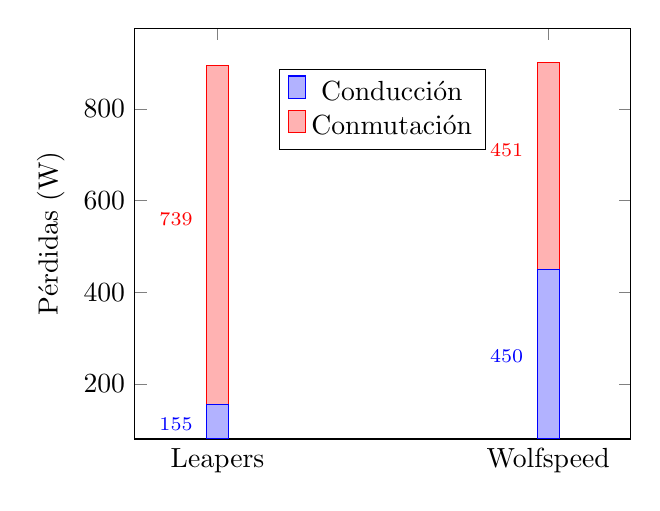
\begin{tikzpicture}
		\begin{axis}[
			ybar stacked,
			width=0.65\textwidth,
			yticklabel style={/pgf/number format/.cd,fixed,fixed zerofill,precision=0,/tikz/.cd},
			ylabel={Pérdidas (W)},
			symbolic x coords={Leapers, Wolfspeed},
			xtick=data,
			bar width=8pt, % Ancho de las barras
			enlarge x limits=0.25, % Espacio adicional a ambos lados de las barras
			nodes near coords,
			nodes near coords align={vertical},
			every node near coord/.append style={font=\scriptsize, xshift=-15pt, yshift=0pt},
			legend style={
				at={(0.5, 0.9)},
				anchor=north,
			},
			]
			\addplot coordinates {(Leapers, 155) (Wolfspeed, 450)};
			\addplot coordinates {(Leapers, 739) (Wolfspeed, 451)};
			\legend{Conducción, Conmutación}
		\end{axis}
	\end{tikzpicture}
	\caption{Comparación de pérdidas de conducción y conmutación}
	\label{fig:loss_comparison}
\end{figure}

Se observa que en el caso de Leapers, las pérdidas de conducción exhiben una significativa disminución en comparación con las de Wolfspeed, mientras que las pérdidas de conmutación muestran un incremento dramático para Leapers en relación con Wolfspeed. Este fenómeno sugiere que, en líneas generales, los dispositivos desarrollados por Leapers podrían ofrecer un camino de corriente más favorable en el semiconductor, y los dispositivos de Wolfspeed son capaces de conmutar más rápido debido a que su carga $Q_G$ es mucho menor, reduciendo así $E_{on}$ y $E_{off}$.

La suma total de las pérdidas de ambos inversores, independientemente del semiconductor, se sitúa entorno a los 900 W, valor con el cual se puede diseñar el sistema de refrigeración.

\subsection{Sistema de Refrigeración}

A continuación se presenta una comparación entre las opciones comunes para refrigerar el inversor:

\begin{table}[H]
	\centering
	\begin{tabular}{|p{2.5cm}|p{5cm}|p{5cm}|}
		\hline
		\textbf{Opción de Refrigeración} & \textbf{Ventajas} & \textbf{Desventajas} \\ \hline
		Convección Natural & Económica, Sin partes móviles & Limitada disipación de calor, Depende del ambiente \\ \hline
		Disipador de Calor & Económico, Fácil de instalar, No requiere energía adicional & Limitado en aplicaciones de alta potencia, Depende del ambiente \\ \hline
		Ventilador & Buena disipación de calor, Control de temperatura & Limitado en aplicaciones de alta potencia, Ruido \\ \hline
		\textit{Coldplate} de Agua & Excelente capacidad de disipación, Buen control de temperatura & Coste, Mantenimiento, Posible riesgo de fugas, Instalación complicada \\ \hline
		\textit{Coldplate} de Aceite & Buena capacidad de disipación, No corrosivo, Alto rango de temperaturas &  Coste, Mantenimiento, Posible riesgo de fugas, Instalación complicada \\ \hline
	\end{tabular}
	\caption{Comparación de Opciones de Refrigeración}
\end{table}



Para el sistema de refrigeración de los semiconductores se ha optado por un sistema de refrigeración líquida consistente en una \textit{coldplate}, una bomba y un radiador. Esta elección se basa en varios factores clave que se detallan a continuación:

\begin{itemize}
	\item \textbf{Mantenimiento de Temperatura:} A diferencia de una refrigeración por aire, una \textit{coldplate} permite mantener una interfaz de temperatura fija para los semiconductores. Esto es crucial para garantizar un funcionamiento estable y confiable de los componentes, especialmente en aplicaciones de alta potencia como la que se está diseñando.
	
	\item \textbf{Experiencia Previa:} El equipo tiene experiencia previa en sistemas de refrigeración líquida, lo que facilita la implementación y mantenimiento de este tipo de sistemas.
	
	\item \textbf{Eficiencia Compacta:} La refrigeración líquida, especialmente con agua, permite un diseño más compacto en comparación con otras opciones. Un disipador haría mucho más voluminoso el convertidor, mientras que la refrigeración líquida permite una distribución más libre de los componentes por el monoplaza. Por ejemplo, se puede situar el radiador en una zona donde tenga mucho contacto con el aire exterior, y conectarlo mediante mangueras a la bomba y a la \textit{coldplate}.
	
	
\end{itemize}

Aunque el carburo de silicio tiene una temperatura máxima de la unión (\(T_{j(max)}\)) notablemente alta, se ha establecido un objetivo de mantener el delta de temperatura (\(\Delta T\)) por debajo de 30 ºC, manteniendo la interfaz térmica del semiconductor a 80ºC como máximo. Este enfoque busca garantizar una operación óptima y una vida útil prolongada de los semiconductores, además de mitigar los posibles efectos negativos derivados del calor.

Se ha elegido agua como el fluido de refrigeración por varias razones:

\begin{itemize}
	\item \textbf{Norma T7.2.2:} Según la norma T7.2.2, los sistemas de refrigeración solo pueden utilizar agua, aire u aceite como refrigerante. Con lo cual, no es posible utilizar líquidos refrigerantes específicos.
	
	\item \textbf{Propiedades Térmicas:} El agua tiene una alta capacidad calorífica y conductividad térmica, lo que la hace eficaz para disipar el calor generado por los semiconductores. El aceite tiene peor conductividad térmica, y su amplio rango de temperaturas no es útil para la aplicación.
	
	\item \textbf{Seguridad:} El agua es un fluido seguro y no inflamable, lo que reduce los riesgos de seguridad en caso de fugas o accidentes. Además, es un fluido fácilmente disponible y de bajo costo en comparación con otros refrigerantes. Si se usa agua destilada, el riesgo de corrosión es más bajo, y los sistemas electrónicos no serán tan susceptibles a posibles fugas.
	
\end{itemize}


\subsection{Gate drivers}

Los gate drivers son componentes críticos en un convertidor de potencia, puesto que son los encargados de conectar las señales débiles de un microcontrolador con los semiconductores. Además, suelen llevar funcionalidades adicionales como la detección de cortocircuitos en el semiconductor, la lectura de señales analógicas de forma aislada, o mecanismos de protección avanzados.

\subsubsection{Funcionamiento Genérico}

Los \textit{gate drivers} desempeñan un papel esencial en la conmutación eficiente de los MOSFETs, proporcionando los niveles de tensión y corriente adecuados para activar y desactivar rápidamente los transistores. 

\subsubsection{Criterios de Selección}

Al seleccionar un \textit{gate driver}, varios factores deben tenerse en cuenta para garantizar un rendimiento óptimo del sistema:

\begin{itemize}
	\item \textbf{Topología}: A pesar de que hay soluciones que incluyen 6 \textit{drivers} en un solo encapsulado, las más comunes son los circuitos integrados diseñados para controlar un solo dispositivo o dos en configuración de medio puente. Sin embargo, encontrar esta última opción para el rango de tensiones de 600 V con características óptimas es difícil. Por lo tanto, la topología más adecuada suele ser la de un solo \textit{driver} por encapsulado.
	\item \textbf{Tensión de aislamiento}: Dado que las señales de puerta vienen del sistema de baja tensión, deben aislarse antes de llegar al \textit{gate}, con lo que será necesario buscar un componente aislado a una tensión adecuada de al menos tres veces superior a la tensión máxima del inversor, 600 V. 
	\item \textbf{Corriente de salida}: Es crucial elegir un \textit{gate driver} que pueda suministrar la corriente necesaria para cargar y descargar rápidamente las capacidades de compuerta de los MOSFETs. La corriente necesaria depende de la resistencia de puerta, pero se puede determinar una primera cota de $\frac{V_{GS,typ}}{R_{G,int}} = \frac{20 \text{V}}{2.4 \Omega} = 8.3 \text{A}$
	\item \textbf{Protecciones integradas}: Funciones como la lectura de señales analógicas, la posibilidad de paralelizar salidas o la inclusión de protecciones son muy beneficiosas para la integración del convertidor.
\end{itemize}

\subsubsection{Comparativa de Alternativas}

A continuación se presenta una comparativa entre varios modelos de \textit{gate drivers}, considerando sus características principales:

\begin{table}[H]
	\centering
	\begin{tabular}{|l|p{3.5cm}|p{3.5cm}|p{3.5cm}|}
		\hline
		\textbf{Características} & \textbf{ADUM4146} & \textbf{UCC21710} & \textbf{GD3160} \\
		\hline
		Voltaje de Operación & -15 V hasta 30 V & –17.5 V hasta 36 V & -12 V hasta 25V \\
		\hline
		Corriente de Salida & 4.61 A & 10 A & 15 A \\
		\hline
		Protecciones & Desaturación, UVLO & Sobrecorriente, Desaturación, \textit{Miller Clamp} & Desaturación, Sobrecorriente, Apagado suave \\
		\hline
		Tiempo de Retardo & 75 ns & 90 ns & - \\
		\hline
		Aislamiento & 5 kV & 5.7 kV & 8 kV \\
		\hline
		Extras & - & Sensor analógico aislado & Sensor analógico aislado \\
		\hline
		CMTI & 100 V/ns & 150 V/ns & 100 V/ns \\
		\hline
	\end{tabular}
	\caption{Comparación de \textit{gate drivers}}
\end{table}

Considerando los criterios de selección, se observa que el UCC21710 se presenta como una opción intermedia adecuada. En primer lugar, la corriente de salida que ofrece es de hasta 10 A, lo que lo hace adecuado para cargar y descargar rápidamente las capacidades de compuerta de los MOSFETs, cumpliendo así con uno de los requisitos fundamentales. Además, integra protecciones contra sobrecorriente y desaturación, así como la funcionalidad de \textit{Miller Clamp}. Además, la inclusión de un sensor analógico aislado proporciona la capacidad de monitorear la temperatura de los semiconductores con sus sensores integrados sin ningún componente adicional.

Aunque las protecciones de sobrecorriente y desaturación son elementos fundamentales para garantizar la seguridad y el correcto funcionamiento de un inversor, en este caso se ha optado por no implementarlas debido a las complicaciones que pueden surgir en el diseño del \textit{layout}. Estas protecciones requieren la inclusión de componentes adicionales con \textit{footprints} grandes y un enrutamiento más complejo de las señales, lo cual puede resultar en problemas de interferencia y aumento de la complejidad del circuito.

Es importante destacar que este inversor se encuentra en una fase inicial de prototipado y desarrollo, donde se prioriza la funcionalidad básica y la viabilidad del diseño. En futuras revisiones y etapas de desarrollo, se considerará la inclusión de estas protecciones, ya que son cruciales para proteger tanto el inversor como los dispositivos conectados. La decisión actual de omitir estas protecciones se basa en la necesidad de simplificar el diseño y garantizar una implementación más eficiente y manejable en esta fase del proyecto.

\begin{figure}[H]
	\centering
	\includegraphics[width=0.7\linewidth]{fig/UCC21710-block}
	\caption{Diagrama de bloques funcional del \textit{gate driver} seleccionado.}
\end{figure}


\subsubsection{Cálculos del Gate Driver Seleccionado}


\begin{itemize}
	
	\item \textbf{Tensión \textit{gate-source}}: Uno de los valores más importantes a determinar es el nivel de tensión de puerta para encender y apagar el MOSFET. En una aplicación \textit{hard-switched} como la del convertidor en diseño, es beneficioso usar una tensión de encendido tan alta como sea posible.
	
	Dada la naturaleza rápida del carburo de silicio, se prevé una dV/dt considerable, la cual puede causar varios problemas. Uno de ellos sería la activación accidental de un MOSFET, la cual causaría la condición de \textit{shoot-through}. Una estrategia para mitigar parcialmente este problema es el uso de un \textit{gate driver} con \textit{Miller Clamp}. Además, se suele apagar el dispositivo utilizando una tensión negativa, que amortigua posibles interferencias en la puerta del dispositivo afectado. El valor de tensión negativo al cual se encuentre la puerta aumenta la tensión que debe inducirse en ese nodo para llegar a la tensión umbral $V_{G,treshold}$ del MOSFET. Dado que el valor óptimo no es trivial, conviene implementar alguna manera de modificarlo, por ejemplo, mediante el uso de un regulador lineal.
	
	Los dispositivos seleccionados tienen un rango de tensiones $V_{GS}$ un tanto distintos, siendo el de Leapers de +21 V a -2 V, y el de Wolfspeed de +15 V a -4 V.
	
	\item \textbf{Potencia de alimentación del \textit{gate driver}:} Se estima en función de la frecuencia de conmutación y la carga de la compuerta de los MOSFETs, además de la tensión $V_{GS}$.
	
	\begin{equation}
	I_{supply, min} = f_{\text{conm}} \cdot Q_G
	\end{equation}
	
	Donde:\\
	- \( I_{supply, min} \) es al corriente mínima que debe poder suministrar la fuente de alimentación del \textit{gate driver},\\
	- \( f_{\text{conm}} \) es la frecuencia de conmutación, y\\
	- \( Q_G \) es la carga en la puerta.\\
	
	
	\[
	I_{supply, min} = f_{\text{conm}}\cdot Q_G = 50 \text{kHz} \cdot 520 \text{nC} = 26 \text{mA}
	\]
	
	Con esta corriente se puede calcular la potencia necesaria de la fuente:
	
	\begin{equation}
		P_{supply, min} = \Delta V_{GS}\cdot I_{supply, min} 	
	\end{equation}
	
	Donde:\\
	- \( P_{supply, min} \) es la potencia mínima que debe poder suministrar la fuente de alimentación del \textit{gate driver} y\\
	- \( \Delta V_{GS} \) es la diferencia entre la tensión de puerta de encendido y apagado.\\
	
	\[
	P_{supply, min} = \Delta V_{GS}\cdot I_{supply, min} = 20 \text{V} \cdot26 \text{mA} = 0.52 \text{W}
	\]
	
	Con esta estimación de potencia mínima requerida, es esencial seleccionar una fuente adecuada para los \textit{gate drivers}. En este contexto, se considera la serie MGJ2 de Murata, que ofrece características como:
	\begin{itemize}
		\item Tensión de entrada de 5 V, 12 V, 15 V o 24 V, lo que permite adaptarse a diferentes fuentes de alimentación disponibles. En esta aplicación, la entrada de 5 V simplifica mucho la arquitectura de \textit{hardware}.
		\item Rango de tensiones de salida muy variados, que permite intercambiar fuentes para probar distintos niveles de tensión.
		\item Aislamiento reforzado hasta 5.2 kVDC, garantizando la seguridad y el cumplimiento de la normativa.
		\item Caracterización de CMTI mayor a 200 V/ns, lo que garantiza una respuesta rápida y efectiva ante transitorios de alta velocidad.
	\end{itemize}
	
	\item \textbf{Valores de Resistencias de Puerta (\(R_{G_{ON/OFF}}\)):} Reducir el valor de las resistencias de puerta conlleva la disminución de las pérdidas de conmutación, ya que los MOSFETs cambiarán más rápido y, por lo tanto, pasarán menos tiempo en la etapa de conmutación. Esta rapidez en el cambio implica un mayor dV/dt, lo que puede ser responsable del aumento de la interferencia electromagnética (EMI). El valor de estas resistencias se estimará mejor con pruebas empíricas, pero se puede partir de un valor de referencia de la hoja de datos, que en este caso es de 3.3 $\Omega$.
	
\end{itemize}


\subsection{Bus de Condensadores}

La tarea del bus de condensadores es equilibrar la potencia instantánea fluctuante en los nodos positivo y negativo de la batería, resultante de los semiconductores que conmutan esta tensión continua en la carga. Estos condensadores, a menudo referidos como bus o enlace de continua, mitigan el rizado creado por la conmutación de alta frecuencia, lo que garantiza un suministro de tensión más estable para el sistema eléctrico en su conjunto.

\subsubsection{Función del Bus de Condensadores}

En un inversor de fuente de voltaje (VSI), el bus de condensadores tiene dos funciones principales:

\begin{itemize}
	\item \textbf{Minimizar el rizado de tensión:} El rizado de tensión en el bus de continua está causado por la conmutación de los dispositivos semiconductores. El bus de condensadores ayuda a reducir este rizado de tensión, lo que es crucial para evitar fluctuaciones en la tensión máxima que se puede consignar al motor.
	
	El rizado de tensión se calcula como:
	
	\begin{equation}
	V_{\text{ripple}} = \frac{I_{\text{C,RMS}}}{C \cdot f_{\text{conm}}}
	\end{equation}
	
	Donde:\\
	- \( V_{\text{ripple}} \) es el rizado de tensión producido,\\
	- \( I_{\text{C,RMS}} \) es la corriente alterna del bus de condensadores,\\
	- \( C \) es la capacitancia del bus de condensadores, y\\
	- \( f_{\text{conm}} \) es la frecuencia de conmutación.\\
	
	\item \textbf{Proporcionar la potencia reactiva:} Además de la reducción del rizado de tensión, los condensadores en el bus también proporcionan potencia reactiva necesaria para compensar la carga inductiva del motor, sobre todo en la región de debilitamiento de campo.
	
\end{itemize}

\subsubsection{Dimensionamiento del Bus de Condensadores}

Para dimensionar adecuadamente el bus de condensadores en un inversor de fuente de voltaje, se deben considerar las siguientes condiciones:

\begin{itemize}
	\item \( V_C > 1.1 \cdot V_{\text{max}} \)
	
	Donde:\\
	- \( V_C \) es el voltaje del bus de condensadores,\\
	- \( V_{\text{max}} \) es la tensión máxima DC.\\
	
	\item \( I_{C,\text{RMS}} \approx 0.65 \cdot I_{\text{phase,RMS}} \)
	
	Donde:\\
	- \( I_{C,\text{RMS}} \) es la corriente efectiva del bus de condensadores,\\
	- \( I_{\text{phase,RMS}} \) es la corriente efectiva de fase,\\
	- El factor 0.65 se utiliza para estimar la corriente RMS máxima del bus de condensadores en el peor caso, que con una modulación SVPWM se da cuando el índice de modulación es de aproximadamente 60\%.\\
	
	\item \( C > \frac{I_{C,\text{RMS}}}{V_{\text{ripple}} \cdot f_{\text{conm}}} \)
	
	Donde:\\
	- \( C \) es la capacitancia del bus de condensadores,\\
	- \( V_{\text{ripple}} \) es el rizado de tensión permitido,\\
	- \( f_{\text{conm}} \) es la frecuencia de conmutación.\\
\end{itemize}

Es fácil ver como reducir la frecuencia de conmutación disminuirá proporcionalmente la corriente nominal para el mismo rizado de tensión o aumentará proporcionalmente el rizado de tensión para la misma corriente de salida.

Ahora, aplicando estas consideraciones a los valores del diseño:

\begin{itemize}
	\item \( V_C > 1.1 \cdot V_{\text{max}} = 1.1 \cdot 600 \text{ V} = 660 \text{ V} \rightarrow 850 \text{ V} \) \\
		Escoger condensadores con un límite de tensión más grande es más seguro para transitorios y el régimen de trabajo en debilitamiento de campo.
	\item \( I_{C,\text{RMS}} \approx 0.65 \cdot I_{\text{phase,RMS}} = 0.65 \cdot 80 \text{ A,RMS} = 52 \text{ A,RMS}\) \\
		Se debe asegurar que el condensador puede soportar esta corriente, idealmente sin refrigeración. En caso de usar múltiples condensadores para formar el bus, la corriente se reparte de forma proporcional entre cada uno de ellos.
	\item \( C > \frac{I_{C,\text{RMS}}}{V_{\text{ripple}} \cdot f_{\text{conm}}} = \frac{52 \text{A,RMS}}{15 \text{V} \cdot 50 \text{kHz}} \approx 79 \mu\text{F} \rightarrow 100 \mu\text{F} \)\\
		Conviene sobredimensionar la capacitancia tanto como sea posible atendiendo a límites mecánicos y de ensamblaje. El valor de $V_{\text{ripple}}$ se suele estimar entre un 5\% y un 10\% de la tensión mínima de funcionamiento, que en este caso es de entorno a los 350 V ($\frac{15 \text{V}}{350 \text{V}} = 4.3\%$).
\end{itemize}

\subsubsection{Selección de Condensadores}

Se ha optado por un diseño con 10 condensadores del modelo FHA85Y106KS de la serie FH de Murata. A continuación se detallan las razones para esta elección:

\begin{itemize}
	\item \textbf{Material:} La serie FH de Murata tiene condensadores de película, cuya resistencia interna es muy inferior a la de un condensador electrolítico, lo cual es crucial para minimizar las pérdidas en el condensador.
	
	\item \textbf{Densidad de capacitancia:} Esta serie de condensadores presenta una alta densidad de capacitancia de entorno a $0.6\frac{\mu F}{cm^3}$. Esto va a permitir compactificar el diseño bastante.
	
	\item \textbf{Tensión máxima:} Con una gama de 500 V y otra 850 V, estos últimos están dentro del rango necesario para operar de manera segura, incluso en debilitamiento de campo.
	
	\item \textbf{Temperatura de Operación:} Tienen un rango de temperatura de operación amplio, que va desde -40°C hasta +125°C. Dado que se prefiere evitar su refrigeración, el hecho de que aguanten altas temperaturas permite tener más confiabilidad en la corriente que pueden soportar y el calentamiento que esta va a provocar.
	
	\item \textbf{Frecuencia de Operación:} Los condensadores FHA85Y106KS están diseñados para operar en frecuencias de hasta 200 kHz, cuatro veces superior a la frecuencia de conmutación escogida.
	
	
\end{itemize}

\begin{figure}[H]
	\centering
	\includegraphics[width=0.7\linewidth]{fig/FHA85Y106KS}
	\caption{Apariencia del condensador seleccionado.}
\end{figure}


Se evalúa el comportamiento térmico utilizando la hoja de datos:
\begin{figure}[H]
	\centering
	\includegraphics[width=0.7\linewidth]{fig/dc-link-temp}
	\caption{Calentamiento propio del condensador en función de la corriente.}
\end{figure}

Dado que hay 10 condensadores, la corriente máxima de cada uno es de $\frac{52 \text{ A,RMS}}{10} = 5.2 \text{A,RMS}$. Por tanto, el incremento de temperatura es de 10 ºC como máximo.

\subsection{Conectores de Potencia}

Para asegurar una conexión segura y eficiente del bus de continua con la batería y de los semiconductores con las fases de los motores, se requiere una cuidadosa selección de conectores. Dada la alta corriente que deben soportar, las conexiones soldadas sin soportes adicionales no son adecuadas según la normativa. Por ello, se opta por la tecnología de conectores \textit{press-fit}.

Un modelo que destaca en esta aplicación es el 7461063 de Würth Elektronik, diseñado para conexiones de hasta 160 A. Está fabricado en latón con una superficie estañada, y su montaje \textit{press-fit} asegura una conexión mecánica y eléctrica sólida.

La tecnología \textit{press-fit} utilizada en estos conectores REDCUBE de Würth Elektronik proporciona una serie de ventajas significativas. Al presionar los pines en la PCB, se genera una soldadura fría homogénea entre el pin y el orificio metalizado, asegurando una resistencia de contacto inferior a 200 $\mu$Ohm.

\begin{figure}[H]
	\centering
	\includegraphics[width=0.35\linewidth]{fig/pressfit}
	\caption{Conector REDCUBE PRESS-FIT - Modelo 7461063.}
\end{figure}

Estos conectores permiten una flexibilidad de integración muy grande, puesto que la conexión a ellos se realiza mediante una unión roscada, un tornillo, lo cual permite conectar cables con terminales de anilla, pletinas y otros elementos conductores. Gracias a esto es muy sencillo implementar mecanismos de bloqueo positivo para evitar la desconexión por vibraciones.

\begin{figure}[H]
	\centering
	\includegraphics[width=0.5\linewidth]{fig/pressfit-980v}
	\caption{Ejemplo de conexión con bloqueo positivo utilizando una tuerca DIN 980V.}
\end{figure}



\subsection{Elección del Sensor de Posición}

AAAAAAAAAAAAAAAAAAAAAAAAAAAAAAAAAAAAAAAAA

\begin{table}[H]
	\centering
	\begin{tabular}{|p{2.5cm}|p{5cm}|p{5cm}|}
		\hline
		\textbf{Sensor de Posición} & \textbf{Ventajas} & \textbf{Desventajas} \\ \hline
		Encoder Incremental (A, B, Z) & Buena precisión angular, Bajo costo, Tamaño compacto & Requiere referencia inicial, Vulnerable a errores por pérdida de pulsos \\ \hline
		Resolver & Alta precisión y resolución, Robusto ante condiciones extremas & Costoso, Voluminoso, Requiere electrónica adicional \\ \hline
		Encoder Seno-Coseno & Alta precisión, Sin error de referencia & Costoso, Requiere electrónica adicional, AAAAAAAAAAAAA a interferencias \\ \hline
		Sensores de Posición por Efecto Hall & Sin contacto mecánico, Robusto, Buena resolución & Menor precisión que otros sensores, Sensible a campos magnéticos externos \\ \hline
	\end{tabular}
	\caption{Comparación de Sensores de Posición}
\end{table}

Para el sistema en cuestión, se ha optado por utilizar un Encoder Incremental con canal de índice (A, B, Z) debido a las siguientes consideraciones:

AAAAAAAAAAAAAAAAAAAAAAAAAAAAAAAAAAAAAAAAAAAAAAAAA


\subsection{Microcontrolador}

\subsection{PCB de potencia}

Esta PCB es una placa de 4 capas que integra componentes de potencia y circuitos de adquisición para el control de un solo motor eléctrico. Se requieren de dos de estas PCBs para montar el convertidor al completo.

\subsubsection{Concepto y Layout}

La PCB de potencia es el sustrato físico sobre el cual se montan y conectan los componentes de potencia. En ella están situados los semiconductores, el bus de condensadores, las medidas de tensión, corriente y temperatura, los \textit{gate drivers}, y algunos circuitos de seguridad. A continuación se muestran unos bocetos iniciales que se usaron para tantear el emplazamiento de los componentes y conexiones de potencia:

\begin{figure}[H]
	\centering
	\begin{minipage}{0.35\textwidth}
		\centering
		\includegraphics[width=\textwidth]{fig/boceto5}
	\end{minipage}\hfill
	\begin{minipage}{0.55\textwidth}
		\centering
		\includegraphics[width=\textwidth]{fig/boceto6}
	\end{minipage}
	\caption{Bocetos del \textit{layout} del inversor.}
	\label{sketches_layout}
\end{figure}


\begin{figure}[H]
	\centering
	\includegraphics[width=0.7\linewidth]{fig/layout}
	\caption{\textit{Layout} de la PCB de potencia, con las zonas más importantes marcadas.}
\end{figure}

En el \textit{layout} se distinguen varias zonas. 
\begin{itemize}
	\item \textbf{Zona 1:} Conector a la PCB de control y protección de la alimentación de baja tensión.
	\item \textbf{Zona 2:} Conectores de las fases del motor y montajes mecánicos.
	\item \textbf{Zonas 3, 4 y 5:} Semiconductores, sensores de corriente, \textit{gate drivers} y \textit{snubbers} para cada fase.
	\item \textbf{Zona 6:} Bus de condensadores, conectores de alta tensión DC, circuito de descarga y sensado de tensión.
\end{itemize}

\subsubsection{Restricciones y enrutado}
Dado que esta PCB implementa partes del circuito del sistema de tracción y partes del sistema de baja tensión, se debe crear una separación física de 4 mm ya que estará acabada con un revestimiento conformal acrílico (\textit{conformal coating}).

Los espaciados entre conductores de la parte de alta tensión son de 3 mm, ya que la tensión que deben aislar es de 600 V. Este valor se obtiene de la norma genérica IPC-2221B, que especifica una separación de $2.5+(V-500)\cdot0.005 \text{mm} = 3 \text{mm}$.

El dimensionamiento de las pistas para la corriente que debe pasar es algo complicado, y de hecho condiciona el apilado de la PCB. Por ello, se selecciona un apilado de 4 capas de 70 micras (2 onzas por pulgada cuadrada).

\begin{figure}[H]
	\centering
	\includegraphics[width=0.7\linewidth]{fig/stackup_power}
	\caption{Apilado de la PCB de potencia}
\end{figure}

Para dimensionar el ancho de estas pistas se ha considerado la corriente RMS de fase, ya que es la corriente máxima en toda la PCB. Después, se ha usado este ancho para todas las conexiones de potencia, aunque la corriente que vean sea menor. El cálculo se ha realizado usando la norma IPC-2152, que especifica unas relaciones de capacidad de corriente respecto a incremento de temperatura y grosor de capa. Ya que el cálculo es algo tedioso, se opta por el uso de una calculadora específica para este propósito:

\begin{figure}[H]
	\centering
	\includegraphics[width=0.7\linewidth]{fig/width}
	\caption{Cálculo del ancho de pista necesario.}
\end{figure}

El resultado es de 10 mm, lo cual es exagerado, pero sin embargo, solamente se está teniendo en cuenta una capa. Por ello, se decide enrutar las conexiones de potencia por un mínimo de 2 capas con un ancho mínimo de 5 mm. A continuación se detalla el enrutado de la conexión DC positiva de uno de los 3 módulos de medio puente:

\begin{figure}[H]
	\centering
	\begin{subfigure}{0.4\linewidth}
		\centering
		\includegraphics[width=\linewidth]{fig/ts+bot}
		\caption{Vista del enrutado de baja corriente (azul), la conexión positiva del bus de continua (naranja) y de la fase A (rosado).}
	\end{subfigure}
	\hfill
	\begin{subfigure}{0.4\linewidth}
		\centering
		\includegraphics[width=\linewidth]{fig/layout2}
		\caption{Detalle de una sección más estrecha.}
	\end{subfigure}
	\caption{Ejemplo de enrutado de la conexión DC positiva del medio puente de la fase A.}
\end{figure}

Como se puede apreciar, el espaciado que hay que dejar por aislamiento compite por espacio con el ancho de las conexiones. En la mayoría de casos se ha podido respetar el ancho mínimo de 5 mm, sin embargo, en algunas situaciones esto no es posible. Por ejemplo, lo ilustrado en la subfigura b muestra una estrechez de 1.5 mm, pero como esa conexión está repetida en dos capas, el ancho total es de 3 mm. Además, la conexión positiva en el semiconductor se realiza a través de dos grupos de pines, y como antes de realizar esa estrechez ya se ha conectado un grupo de pines, se puede asumir que la corriente que circula por ese trozo de cobre es la mitad que la corriente continua entera que va a recibir ese módulo, que a su vez, es aproximadamente un tercio de la corriente continua total ($\frac{1}{3}\frac{17.5 \text{kW}}{450 \text{V}} = 13 \text{A}$), pasado por la calculadora, tan solo son necesarios 2.8 mm de cobre para esa corriente, lejos de los 10 mm que se han intentado mantener.

Esto es tan solo un ejemplo del análisis que se ha realizado con cualquier mínima sospecha de falta de cobre en todo el enrutado de potencia. Un camino de corriente muy estrecho podría presentar sobrecalentamiento y en casos extremos, levantamiento de la pista o plano.

\subsubsection{Bloques Funcionales}

La PCB de potencia se divide en varios bloques funcionales, que se juntan en un esquemático jerárquico, que además incluye la conexión entre estos bloques, algunas notas indicativas y componentes que no pertenecen a ningún bloque en específico:

\begin{figure}[H]
	\centering
	\includegraphics[width=0.8\linewidth]{fig/schPower1}
	\caption{Esquemático jerárquico de la PCB de Potencia}
\end{figure}

En el esquemático se pueden distinguir el conector a la PCB de control, la protección de alimentación de baja tensión y unas notas indicativas, así como una leyenda de colores. Se anotan también los cambios y la fecha en la que se envía a producción. Los bloques que se pueden ver incluyen:

\begin{itemize}
	
	\item \textbf{Etapa de Potencia:} En este bloque aparecen los semiconductores, el bus de condensadores y una descarga pasiva.
	
	\item \textbf{Sensado de corriente:} Se incluyen los sensores de corriente y su interfaz analógica con la PCB de control.
			
	\item \textbf{\textit{Gate Drivers}:} En este bloque se recogen las señales necesarias para la conmutación, así como la configuración de los \textit{gate drivers} en su conjunto. Este bloque contiene 3 subcircuitos correspondientes con cada fase. En ellos se encuentran los \textit{gate drivers} en sí, junto a su alimentación aislada, los \textit{snubbers} y la medida de temperatura.
		
	\item \textbf{DC:} Por último, hay un bloque dedicado al bus de continua, que incluye el circuito de descarga, la medida de tensión y la detección de 60 V requerida por la normativa.
\end{itemize}

\subsubsection{Circuitos Importantes}

\textbf{VSI}
Ya que los módulos son estructuras \textit{half-bridge}, se deben conectar entre sí para formar la topología VSI.
\begin{figure}[H]
	\centering
	\includegraphics[width=0.7\linewidth]{fig/VSI-shc}
	\caption{Conexión de los módulos configurando un VSI.}
\end{figure}

\textbf{Protección de alimentación}
Aunque en principio es regulada, la entrada de 5 V necesita de un mínimo de protecciones sencillas para evitar retrasos ocasionados por fallos mientras se realizan pruebas. En este caso se ha usado un fusible como protección contra sobrecorriente, un diodo \textit{zener} a modo de protección contra sobretensión (hará saltar el fusible cuando la tensión de entrada supere la tensión umbral), y un diodo \textit{schottky} como protección frente a tensión inversa, ya que tiene poca caída de tensión, actúa bastante rápido y es barato.
\begin{figure}[H]
	\centering
	\includegraphics[width=0.5\linewidth]{fig/5V-sch}
	\caption{Circuito de protección de alimentación.}
\end{figure}

\textbf{Alimentación del \textit{gate driver}}

\begin{figure}[H]
	\centering
	\includegraphics[width=0.9\linewidth]{fig/GD-supp-sch}
	\caption{Alimentación bipolar aislada del \textit{gate driver}.}
\end{figure}

En función del modelo de DCDC específico escogido de la serie MGJ2 de Murata, se tendrá una tensión positiva y negativa diferente. La tensión positiva no es muy problemática puesto que se pueden seleccionar DCDCs con salidas de +18 V o de +15 V, valores que encajan con los recomendados por los fabricantes de los semiconductores.

Sin embargo, ese no es el caso para las tensiones negativas, ya que el valor debería poder ajustarse para ser más versátil en el desarrollo. Por ello, se implementan reguladores lineales para ajustar $V_{EE,HS}$ y $V_{EE,LS}$ durante las pruebas para afinar el voltaje negativo necesario.

$V_{EE}$ se calcula como:

\[ V_{EE,LS} = -1.186 \cdot \left(1 + \frac{R1}{R2}\right) \]

Donde \( R1 + R2 \approx 100 \text{k}\Omega \) según la hoja de datos del LDO. Para las configuraciones específicas de Leapers y Wolfspeed, los valores de las resistencias son los siguientes:

\begin{itemize}
	\item Leapers: \( R1 = 36 \text{k}\Omega \), \( R2 = 56 \text{k}\Omega \)
	\item Wolfspeed: \( R1 = 68 \text{k}\Omega \), \( R2 = 30 \text{k}\Omega \)
\end{itemize}

Este proceso permite ajustar de forma precisa los voltajes negativos necesarios para el correcto funcionamiento del circuito de conmutación.


\textbf{\textit{Gate driver}}
\begin{figure}[H]
	\centering
	\includegraphics[width=0.9\linewidth]{fig/GD-sch}
	\caption{\textit{Gate driver} con medida de temperatura y \textit{snubbers}.}
\end{figure}

Uno de los componentes más importantes de todo el diseño tiene una de las implementaciones más sencillas, ya que la hoja de datos del UCC21710 proporciona mucha información útil para la aplicación final.

El \textit{gate driver} UCC21710 se implementa con varias características que lo hacen adecuado para su uso en aplicaciones de potencia. Las señales TRIP y OK están configuradas en \textit{open drain}, lo que permite que se paralelicen con los otros \textit{gate drivers} para facilitar su integración. La entrada IN- no se utiliza y está conectada a tierra. El pin ENABLE se controla desde el MCU, y cuando se fuerza un estado bajo durante más de 1 $\mu$s, se resetea la señal TRIP. La señal TRIP se lee como una interrupción externa desde el MCU, y sirve para detectar un error en los \textit{gate drivers} y actuar rápidamente.

Para la medición de temperatura, se utilizan los \textit{drivers} de los MOSFETS del \textit{low-side}. Estos proporcionan una corriente de salida de 200 $\mu$A en su salida, a través de la cual se puede interpretar la medida. Esta señal se convierte a PWM y luego a analógica mediante un filtro RC para ser recibida directamente por el ADC del MCU. 

El circuito de medición de temperatura utiliza el sensor NTC del semiconductor para obtener una lectura de tensión, la cual se convierte en una lectura de bits mediante el ADC del MCU. La relación entre la resistencia del NTC y la temperatura se modela utilizando la fórmula de Steinhart-Hart, que toma en cuenta el valor de Beta del NTC, la resistencia a una temperatura de referencia, y la temperatura ambiente. La fórmula utilizada es:

\[
NTC = R_0 \cdot e^{\left[-\beta \cdot \left(\frac{1}{T_0} - \frac{1}{\text{T}}\right)\right]}
\]

El voltaje leído por el ADC se calcula con la siguiente fórmula:
\[
V_{\text{read}} = V_{\text{CC,GD}} \cdot \left(\frac{-20 \cdot I_{\text{AIN}} \cdot (R_{\text{filt}} + NTC)}{100}\right) = 5 \text{V} \cdot \left(\frac{-20 \cdot 200 \mu\text{A} \cdot (10 \text{k}\Omega + NTC)}{100}\right)
\]

El circuito también incluye protección de \textit{Miller clamp} para evitar activaciones accidentales de los MOSFETs. Aunque los \textit{gate drivers} tienen un \textit{pull-down} activo, se ha implementado un \textit{pull-down} externo con $R_{GS,HS}$ y $R_{GS,LS}$. Sin embargo, la detección de sobrecorriente no está implementada en este diseño por los motivos mencionados en un apartado anterior.

Adicionalmente, se incluyen unos \textit{snubbers} consistentes en un RC entre drenador y fuente, un condensador entre puerta y drenador y un condensador entre puerta y fuente. En caso de encontrar problemas excesivos con la conmutación, pueden ayudar a amortiguar transitorios.

Cabe destacar que el enrutado de este subcircuito es especialmente crítico por los parásitos inductivos que se pueden ocasionar. En particular, la inductancia en el camino de retorno de puerta-fuente puede ser fatal para el comportamiento de la conmutación, razón por la cual se ha tirado un plano conectado a la fuente de cada MOSFET en el área donde se enruta su \textit{driver}, para minimizar esa inductancia. En estas líneas, se ha enrutado en orden de prioridad, empezando por la conexión de las puertas de los MOSFETs a los \textit{drivers} y la alimentación aislada, y acabando con los \textit{snubbers}.

\begin{figure}[H]
	\centering
	\includegraphics[width=0.7\linewidth]{fig/invPowerRouting}
	\caption{Enrutado en la capa superior de un \textit{half-bridge}.}
\end{figure}

Otro camino susceptible a ser causa de \textit{overshoot} es el que forman los AAAAAAAAAAAAAAAAAAAAAAAAAAAAAAAAAAAAAAAAAAAAAAAA


\textbf{Descarga}
\begin{figure}[H]
	\centering
	\includegraphics[width=0.9\linewidth]{fig/discharge-sch}
	\caption{Circuito de descarga.}
\end{figure}

Una de las partes más importantes en cuanto a la seguridad eléctrica es la implementación del circuito de descarga. Este circuito se utiliza para descargar la energía almacenada en el bus de condensadores cuando el convertidor no está operativo. Los requisitos de la normativa son que el circuito debe ser capaz de descargar el bus de la tensión máxima hasta 60 V en menos de 5 segundos. Adicionalmente, el circuito debe ser capaz de aguantar de forma constante la tensión máxima.

Con tal de cumplir estos requisitos se ha optado por un circuito basado en un NMOS, cuya puerta se conecta al terminal positivo del bus a través de una resistencia de valor elevado y se limita la tensión con un diodo \textit{zener}. La puerta del MOSFET está controlada por un optoacoplador de forma aislada desde el circuito de baja tensión. Mientras el bus tenga una tensión superior a 10 V y el optoacoplador esté desactivado, el MOSFET quedará cerrado, conectando el banco de resistencias a los condensadores, descargándolos.

La selección de la resistencia se ha basado en minimizar el tamaño de la misma. La solución más óptima se ha encontrado en utilizar un banco de 24 resistencias SMD de 470k$\Omega$, en encapsulado 2512, que es capaz de disipar 1 W. Se conectan en paralelo para llegar al valor necesario para cumplir con el requisito de tiempo de descarga. Para el cálculo del tiempo de descarga se utiliza la siguiente expresión:
\begin{equation}
	t_{\text{dis}} = R_{\text{dis}} \cdot C \cdot \ln\left(\frac{V_{\text{inicial}}}{V_{\text{final}}}\right)
\end{equation}

\[
t_{\text{dis}} = R_{\text{dis}} \cdot C \cdot \ln\left(\frac{V_{\text{inicial}}}{V_{\text{final}}}\right) = \left(\frac{470 \text{k}\Omega}{24}\right) \cdot (100 \mu\text{F}) \cdot \ln\left(\frac{600 \text{V}}{60 \text{V}}\right) = 4.509 \text{s}
\]

La potencia disipada en cada resistencia de descarga se calcula como:

\begin{equation}
	P(R_{\text{dis}}, \text{max}) = \frac{V_{\text{max}}^2}{R_{\text{dis}}} 
\end{equation}

\[
P(R_{\text{dis}}, \text{max}) = \frac{V_{\text{max}}^2}{R_{\text{dis}}} = \frac{600\text{ V}^2}{470 \text{k}\Omega} = 0.766 \text{W} < 1 \text{W}
\]

\textbf{Medida de corriente}

\begin{figure}[H]
	\centering
	\includegraphics[width=0.8\linewidth]{fig/Imeas-sch}
	\caption{Sensor de corriente de fase.}
\end{figure}

Uno de los componentes más críticos para asegurar el funcionamiento óptimo del inversor es la medición precisa de corriente. En inversores de bajo coste, comúnmente se emplean resistencias \textit{shunt} junto con amplificadores aislados para esta tarea. Sin embargo, esta solución puede presentar diversos desafíos de integración.

Una opción destacada para abordar esta necesidad de medición de corriente es la gama de sensores CKSR-NP de LEM. Este sensor utiliza la tecnología de transductores de corriente basados en \textit{fluxgate}. Sus características incluyen un rango de medición amplio de hasta $\pm$150 A para modelo seleccionado, junto con una alta precisión del 0.8\%. Además, su diseño compacto y montaje en PCB lo hacen ideal para aplicaciones donde se requiere una medición precisa y confiable de corriente en un espacio limitado.

Dado que el sensor tiene un rango de medida de $\pm$150 A y está alimentado a 5 V, se puede pasar por un divisor resistivo con tal de adecuar la señal de salida al rango de entrada del ADC del MCU. Adicionalmente, se puede modificar la tensión de referencia (salida a 0 A) para ajustar todavía más la medida.

\begin{figure}[H]
	\centering
	\includegraphics[width=0.5\linewidth]{fig/cksr50}
	\caption{Sensor de corriente LEM CKSR 50-NP}
\end{figure}


\textbf{Medida de tensión}

\begin{figure}[H]
	\centering
	\includegraphics[width=0.8\linewidth]{fig/Vmeas-sch}
	\caption{Circuito de medida y detección de tensión DC.}
\end{figure}

El monitoreo de la tensión es una tarea crítica en el sistema, ya que no solo es esencial para el control del motor, sino también para la detección y alerta de niveles altos de tensión. Para ambos propósitos, se emplea un divisor de tensión utilizando una serie de resistencias. A continuación se presentan los cálculos del divisor de tensión:

\[ V_{DC,div} = \left(TS^+ - TS^-\right) \cdot \left( \frac{4.7 \text{ k}\Omega}{4.7 \text{ k}\Omega + 6 \cdot 68 \text{ k}\Omega} \right) \]

Sustituyendo los valores de 600 V y 60 V para TS+ y TS-, respectivamente:
\[ V_{DC,div} = \frac{600 \text{ V} \cdot 4.7 \text{ k}\Omega}{4.7 \text{ k}\Omega + 6 \cdot 68 \text{ k}\Omega} = 6.833 \text{ V} \]
\[ V_{DC,div} = \frac{60 \text{ V} \cdot 4.7 \text{ k}\Omega}{4.7 \text{ k}\Omega + 6 \cdot 68 \text{ k}\Omega} = 683 \text{ mV} \]

El valor de potencia disipada en las resistencias de 68k$\Omega$ se calcula como:
\[ P_{R68k} = I_{R68k}^2 \cdot R68k = \left( \frac{V_{DC,div}}{R68k} \right)^2 \cdot R68k = 144 \text{ mW} \]
Se elige un paquete 1206 para las resistencias de 68k$\Omega$, que es capaz de disipar por lo menos 250 mW.

El amplificador aislado ISO224 se utiliza para medir la tensión en el bus de continua. Según la hoja de datos, la salida se calcula como un tercio del voltaje de entrada del divisor de tensión:
\[ (V_{DC,sns+} - V_{DC,sns-}) = \frac{1}{3} \cdot V_{DC,div} = \frac{1}{3} \cdot \left( (TS^+ - TS^-) \cdot \frac{4.7 \text{ k}\Omega}{4.7 \text{ k}\Omega + 6 \cdot 68 \text{ k}\Omega} \right) \]
\[ (V_{DC,sns+} - V_{DC,sns-}) = \frac{1}{3} \cdot 0.011388 \cdot (TS^+ - TS^-) \]
\[ (V_{DC,sns+} - V_{DC,sns-}) = \frac{1}{3} \cdot 0.011388 \cdot 600 \text{ V} = 2.278 \text{ V} \]

El amplificador aislado ISO224 es una elección eficaz para esta aplicación, ya que permite medir de manera precisa la diferencia de potencial entre los terminales, proporcionando un voltaje de salida proporcional a la tensión medida y cuadrando con el rango de adquisición del ADC. Adicionalmente, la salida es diferencial, lo que permite mayor inmunidad frente a interferencias al ser enrutada hasta la placa de control. En ella se deberá incluir un amplificador diferencial o similar para llevar la lectura al ADC.

\subsubsection{Resultado Final}

Tras haber creado todos los subcircuitos, haber emplazado cada componente y enrutado cada nodo, se ha completado el diseño de la placa de potencia. La distribución de componentes permite empaquetar dos de estas placas enfrentadas de forma muy compacta, dejando el espacio justo entre medias para la inserción de la \textit{coldplate}. La placa de control se podrá conectar a las dos de potencia mediante conectores placa a placa, quedando a uno de las caras libres. Por la otra cara se deben incluir las conexiones de potencia DC y la entrada y salida de agua.

\begin{figure}[H]
	\centering
	\begin{subfigure}{0.45\linewidth}
		\centering
		\includegraphics[width=\linewidth]{fig/invPower1}
		\caption{Vista superior.}
	\end{subfigure}
	\hspace{0.05\linewidth} % Espacio horizontal entre subfiguras
	\begin{subfigure}{0.45\linewidth}
		\centering
		\includegraphics[width=\linewidth]{fig/invPower2}
		\caption{Vista inferior.}
	\end{subfigure}
	\caption{Vistas 3D de la PCB de potencia.}

\end{figure}


\begin{figure}[H]
	\centering
	\begin{subfigure}{0.45\linewidth}
		\centering
		\includegraphics[width=\linewidth]{fig/invPower3}
		\caption{Vista frontal, conexión del bus DC y \textit{coldplate}.}
	\end{subfigure}
	\hspace{0.05\linewidth} % Espacio horizontal entre subfiguras
	\begin{subfigure}{0.45\linewidth}
		\centering
		\includegraphics[width=\linewidth]{fig/invPower4}
		\caption{Vista trasera, conexión de la placa de control.}
	\end{subfigure}
	\caption{Vistas 3D del ensamblaje de dos PCBs de potencia.}
	
\end{figure}


\subsection{PCB de control}

explicacion del concepto y de la(s) PCB

justificacion de conectores / interfaces

justificacion numero de capas, etc.


\section{\textit{Software}}

\subsection{Concepto}

Diagrama de bloques de software, justificado (ojo, detallar el dual)


\subsection{Tareas}

Init

ADCs

Comunicaciones

PWMs

Flash o EEPROM

Seguridad

\subsection{Interfaz de usuario}

justificar ausencia de UI integrada

Interfaz de HW 

PlotJuggler

Debugger

Actualizacion de parametros por CAN
